%% Commands for TeXCount
%TC:macro \cite [option:text,text]
%TC:macro \citep [option:text,text]
%TC:macro \citet [option:text,text]
%TC:envir table 0 1
%TC:envir table* 0 1
%TC:envir tabular [ignore] word
%TC:envir displaymath 0 word
%TC:envir math 0 word
%TC:envir comment 0 0

\documentclass[acmsmall,screen,review]{acmart}

\usepackage{syntax}
\renewcommand{\syntleft}{\normalfont\itshape}
\renewcommand{\syntright}{\normalfont\itshape}

\usepackage{prftree}

\usepackage{listings}
\usepackage{xcolor}
\usepackage{caption}
\usepackage{subcaption}
\usepackage{fancyvrb}
\usepackage{enumitem}
\usepackage{string-diagrams}
\usepackage{cancel}
\usetikzlibrary{calc}

\definecolor{codegreen}{rgb}{0,0.6,0}
\definecolor{codegray}{rgb}{0.5,0.5,0.5}
\definecolor{codepurple}{rgb}{0.58,0,0.82}
\definecolor{backcolour}{rgb}{0.95,0.95,0.92}

\lstdefinestyle{mystyle}{
%    backgroundcolor=\color{backcolour},   
    commentstyle=\color{codegreen},
    keywordstyle=\color{magenta},
    numberstyle=\tiny\color{codegray},
    stringstyle=\color{codepurple},
    basicstyle=\ttfamily\footnotesize,
    breakatwhitespace=false,         
    breaklines=true,                 
    captionpos=b,                    
    keepspaces=true,                 
    numbers=left,                    
    numbersep=5pt,                  
    showspaces=false,                
    showstringspaces=false,
    showtabs=false,                  
    tabsize=2
}

\lstset{style=mystyle}

\newcounter{todos}
\newcommand{\TODO}[1]{{
  \stepcounter{todos}
  \begin{center}\large{\textcolor{red}{\emph{TODO \arabic{todos}:} #1}}\end{center}
}}
\newcommand{\sorry}{\textcolor{red}{\emph{sorry}}}

\newcommand{\todo}[1]{\stepcounter{todos} \textcolor{red}{TODO \arabic{todos}: #1}}

% Math fonts
\newcommand{\mc}[1]{\ensuremath{\mathcal{#1}}}
\newcommand{\mb}[1]{\ensuremath{\mathbf{#1}}}
\newcommand{\ms}[1]{\ensuremath{\mathsf{#1}}}

% Math
\newcommand{\nats}{\mathbb{N}}

% Syntax atoms
\newcommand{\lbl}[1]{{`#1}}
\newcommand{\lto}{:}
\newcommand{\linl}[1]{\iota_l\;{#1}}
\newcommand{\linr}[1]{\iota_r\;{#1}}
\newcommand{\labort}[1]{\ms{abort}\;{#1}}

% Syntax
\newcommand{\letexpr}[3]{\ensuremath{\ms{let}\;#1 = #2;\;#3}}
\newcommand{\caseexpr}[5]{\ms{case}\;#1\;\{\linl{#2} \lto #3, \linr{#4} \lto #5\}}
\newcommand{\letstmt}[3]{\ensuremath{\ms{let}\;#1 = #2; #3}}
\newcommand{\brb}[2]{\ms{br}\;#1\;#2}
\newcommand{\ite}[3]{\ms{if}\;#1\;\{#2\}\;\ms{else}\;\{#3\}}
\newcommand{\casestmt}[5]{\ms{case}\;#1\;\{\linl{#2} \lto #3, \linr{#4} \lto #5\}}
\newcommand{\where}[2]{#1\;\ms{where}\;#2}
\newcommand{\wbranch}[3]{#1(#2) \lto \{#3\}}
\newcommand{\cfgsubst}[1]{\ms{cfgs}\;\{#1\}}
\newcommand{\wseq}[2]{{#1} \mathbin{{;}{;}} {#2}}
\newcommand{\upg}[1]{{#1}^\uparrow}

% Judgements
\newcommand{\cwk}[2]{#1 \mapsto #2}
\newcommand{\lwk}[2]{#1 \rightsquigarrow #2}
\newcommand{\thyp}[3]{#1 : {#2}^{#3}}
\newcommand{\bhyp}[2]{#1 : #2}
\newcommand{\lhyp}[2]{#1(#2)}
\newcommand{\rle}[1]{{\scriptsize\textsf{#1}}}
\newcommand{\hasty}[4]{#1 \vdash_{#2} #3: {#4}}
\newcommand{\haslb}[3]{#1 \vdash #2 \rhd #3}
\newcommand{\shaslb}[3]{#1 \vdash_{\ms{s}} #2 \rhd #3}
\newcommand{\isop}[4]{#1 \in \mc{I}_{#4}(#2, #3)}
\newcommand{\issubst}[3]{#1: #2 \mapsto #3}
\newcommand{\lbsubst}[4]{#1 \vdash #2: #3 \rightsquigarrow #4}
\newcommand{\teqv}{\approx}
\newcommand{\tmeq}[5]{#1 \vdash_{#2} #3 \teqv #4 : {#5}}
\newcommand{\lbeq}[4]{#1 \vdash #2 \teqv #3 \rhd {#4}}
\newcommand{\tmseq}[4]{\issubst{#1 \teqv #2}{#3}{#4}}
\newcommand{\lbseq}[5]{\lbsubst{#1 \teqv #2}{#3}{#4}{#5}}
\newcommand{\brle}[1]{{\scriptsize\textsf{#1}}}

% Denotational semantics
\newcommand{\dnt}[1]{\llbracket{#1}\rrbracket}
\newcommand{\ednt}[1]{\left\llbracket{#1}\right\rrbracket}
\newcommand{\tmor}[1]{{!}_{#1}}
\newcommand{\dmor}[1]{{\Delta}_{#1}}

% Composition
\newcommand{\invar}{\square}
\newcommand{\outlb}{\blacksquare}

% Weak memory
\newcommand{\bufloc}[1]{\overline{#1}}

% Branding
\newcommand{\isotopessa}{\(\lambda_{\ms{SSA}}\)}

%% Rights management information.  This information is sent to you
%% when you complete the rights form.  These commands have SAMPLE
%% values in them; it is your responsibility as an author to replace
%% the commands and values with those provided to you when you
%% complete the rights form.
\setcopyright{acmcopyright}
\copyrightyear{2024}
\acmYear{2024}
\acmDOI{XXXXXXX.XXXXXXX}

%%
%% These commands are for a JOURNAL article.
% \acmJournal{JACM}
% \acmVolume{37}
% \acmNumber{4}
% \acmArticle{111}
% \acmMonth{8}

%%
%% Submission ID.
%% Use this when submitting an article to a sponsored event. You'll
%% receive a unique submission ID from the organizers
%% of the event, and this ID should be used as the parameter to this command.
%%\acmSubmissionID{123-A56-BU3}

\begin{document}

\title{The Denotational Semantics of SSA}

\author{Jad Ghalayini}
\email{jeg74@cl.cam.ac.uk}
\orcid{0000-0002-6905-1303}

\author{Neel Krishnaswami}
\email{nk480@cl.cam.ac.uk}
\orcid{0000-0003-2838-5865}

\begin{abstract}
  ...
\end{abstract}

\begin{CCSXML}
  <ccs2012>
  <concept>
  <concept_id>10003752.10010124.10010131.10010133</concept_id>
  <concept_desc>Theory of computation~Denotational semantics</concept_desc>
  <concept_significance>500</concept_significance>
  </concept>
  <concept>
  <concept_id>10003752.10010124.10010131.10010137</concept_id>
  <concept_desc>Theory of computation~Categorical semantics</concept_desc>
  <concept_significance>500</concept_significance>
  </concept>
  <concept>
  <concept_id>10003752.10003790.10011740</concept_id>
  <concept_desc>Theory of computation~Type theory</concept_desc>
  <concept_significance>500</concept_significance>
  </concept>
  </ccs2012>
\end{CCSXML}

\ccsdesc[500]{Theory of computation~Denotational semantics}
\ccsdesc[500]{Theory of computation~Categorical semantics}
\ccsdesc[500]{Theory of computation~Type theory}

%%
%% Keywords. The author(s) should pick words that accurately describe
%% the work being presented. Separate the keywords with commas.
\keywords{SSA, Categorical Semantics, Elgot Structure, Effectful Category}

% \received{20 February 2007}
% \received[revised]{12 March 2009}
% \received[accepted]{5 June 2009}

\maketitle

\section{Introduction}

Static single assignment form, or SSA form, has been the dominant compiler intermediate
representation since its introduction by \citet{alpern-ssa-original-88} and \citet{rosen-gvn-1988}
in the late 1980s. Every major compiler -- GCC, Clang, MLIR, Cranelift -- uses this representation,
because it makes many optimizations much easier to do than traditional 3-address code IRs.

The key idea behind SSA is to adapt an idea from functional programming: namely, every variable is
defined only once. This means that substitution is unconditionally valid, without first requiring a
dataflow analysis to compute where definitions reach. Unlike in functional programming, though,
scoping of definitions in SSA is traditionally not lexical. Instead, scoping is determined by
\emph{dominance}: every variable occurence must be dominated by a single assignment in the control
flow graph.

The semantics of SSA has traditionally been handled quite informally, because conceptually, it is a
simple first-order imperative programming language. As a result, whether a rewrite is sound or not
is usually obvious, without having to do a complex correctness argument.

Unfortunately, computers are no longer as simple as they were in the late 1980s. Modern computers
are typically multicore, and feature many levels of caching, and as a result the semantics of memory
is no longer correctly modelled as a big array of bytes. Finding good semantics for modern weak
memory systems remains an ongoing challenge.

As a result, it is not correct to justify compiler optimizations in terms of a simple imperative
model, and it is an open question which equations should hold of an SSA program. This is a
particularly fraught question, because it is also unclear which equations weak memory models should
satisfy.

What we would like to know is which equations any SSA representation should satisfy. This would let
us establish a contract between compiler writers and hardware designers. The compiler writers could
rely upon the equational theory of SSA when justifying optimizations, without needing to know all
the details of the memory model at all times.  Conversely, memory models could be validated by
seeing if they satisfy the equations of SSA, without needing to study every possible compiler
optimization.

Concretely, our contributions are as follows: 

\begin{itemize}
\item First, we give a type-theoretic presentation of SSA, with both typing rules (in
  Section~\ref{sec:typing}) and an equational theory (in Section~\ref{sec:equations}) for
  well-typed terms. We also prove the correctness of suitable substitution properties for this
  calculus. 
  
\item Next, in Section~\ref{sec:densem}, we give a categorical semantics for this type theory, in
  terms of distributive Elgot categories. We show that any denotational model with this categorical
  structure is also a model of SSA. This shows that all of the equations we give are sound with
  respect to the categorical structure. 

\item We also show, in Section~\ref{ssec:completeness}, that syntax quotiented by the equational
  theory yields the initial distributive Elgot category. This establishes that our set of syntactic
  equations is complete, and that there are no equations which the denotational semantics validates,
  but which cannot be proved syntactically. 

\item We proceed in Section~\ref{sec:concrete} to show that this denotational axiomatization is
  useful in practice, by giving a variety of concrete models, including a model of TSO weak memory
  based on~\citet{sparky} in Section~\ref{ssec:tso}. This demonstrates that it is possible to give
  realistic weak memory models which do not disturb the structure of SSA in fundamental ways.

\item Finally, we have substantially mechanized our proofs using the Lean 4 proof assistant. We have
  mechanized proofs of substitution for our type theory, as well as proofs that the syntax forms the
  initial model, and that the SPARC TSO semantics forms a valid model of SSA. The denotational
  semantics and its proof of the soundness of substitution are done on paper. 

\end{itemize}

\section{Static Single Assignment Form}

In this section, we describe SSA form and the isomorphism between the standard $\phi$-node-based
presentation and the more functional \emph{basic blocks with arguments} format. We then discuss
standard dominance-based scoping and how it can be recast as lexical scoping to make it more
amenable to standard type-theoretic treatment. We further generalize this format to allow branching
to arbitrary code rather than only labels, obtaining \emph{A-normal form}
(ANF)~\cite{flanagan-93-anf}, analogously to the transformation described by
\citet{chakravarty-functional-ssa-2003}. A straightforward argument shows that this adds no
expressive power. Finally, to allow for substitution, we relax our syntax to permit arbitrary
expression nesting and \ms{let}-expressions, resulting in \emph{type-theoretic SSA}, or
\isotopessa{}, which will be the focus of the rest of this paper.

As a running example, consider the simple imperative program to compute $10!$ given in
Figure~\ref{fig:fact-program}. 

Operating directly on an imperative language can be challenging, since having a uniform
representation of code friendly to mechanized optimization and analysis is often in tension with
features designed to improve readability and programmer productivity, such as syntax sugar. Early
work on compiler intermediate representations, notably by Frances Allen~\cite{allen-70-cfa},
introduced \emph{three-address code}, also known as \emph{register transfer language (RTL)},  to
normalize programs into a form more suitable for analysis and optimization. We can normalize our
code into 3-address code, as in Figure~\ref{fig:fact-3addr}, by:
\begin{itemize}
  \item Converting structured control flow (e.g., \ms{while}) into unstructured jumps between basic
  blocks labeled \ms{start}, \ms{loop}, and \ms{body}.
  \item Replacing subexpressions like $i + 1$ in $a * (i + 1)$ with \ms{let}-bindings so that every
  expression in our program is atomic.
\end{itemize}

\begin{figure}
  \begin{subfigure}[t]{.5\textwidth}
    \begin{align*}
      & \ms{let}\;n = 10; \\
      & \ms{let\;mut}\;i = 1; \\
      & \ms{let\;mut}\;a = 1; \\
      & \ms{while}\;i_0 < n\;\{ \\
      & \quad a = a * (i + 1) \\
      & \quad i = i + 1; \\
      & \} \\
      & \ms{ret}\;a \\
    \end{align*}
    \caption{As an imperative program}
    \label{fig:fact-imp}
  \end{subfigure}%
  \begin{subfigure}[t]{.5\textwidth}
    \begin{align*}
      \ms{start}:\quad  & \ms{let}\;n = 10; \\
                        & \ms{let\;mut}\;i = 1; \\
                        & \ms{let\;mut}\;a = 1; \\
                        & \ms{br}\;\ms{loop} \\
      \ms{loop}: \quad  & \ms{if}\;i < n\;
                          \{\;\ms{br}\;\ms{body}\;\}\;
                          \ms{else}\;\{\;\ms{ret}\;a\;\} \\
      \ms{body}: \quad  & \ms{let}\;t = i + 1; \\
                        & a = a * t; \\
                        & i = i + 1; \\
                        & \ms{br}\;\ms{loop}
    \end{align*}
    \caption{As 3-address code}
    \label{fig:fact-3addr}
  \end{subfigure}
  \caption{
    A simple, slightly suboptimal program to compute $10!$ via multiplication in a loop, represented
    as typical imperative code and in 3-address code.
  }
  \Description{}
  \label{fig:fact-program}
\end{figure}


Despite this normalization, many optimizations remain difficult to express in this format because a
variable's value may be set by multiple definitions throughout the program's execution. To improve
our ability to reason about programs, we introduce the \emph{static single assignment} restriction,
originally proposed by \citet{alpern-ssa-original-88} and popularized by
\citet{cytron-ssa-intro-91}, which states that every variable must be defined at exactly one point
in the program. We can intuitively represent this as every variable being given by an immutable
\ms{let}-binding.

However, expressing programs with loops in this format is challenging because the value of a
variable may change with each loop iteration. The classical solution is to introduce
\emph{$\phi$-nodes}, which select a value based on the predecessor block from which control arrived.
For example, in basic block \ms{loop} in Figure~\ref{fig:fact-ssa}, $i_0$ evaluates to 1 if we came
from \ms{start} and to $i_1$ if we came from \ms{body}. Similarly, $a_0$ evaluates to either 1 or
$a_1$ based on the predecessor block. This mechanism allows us to maintain the single-assignment
property while capturing control-flow-dependent variable updates.

Notably, $i_1$ and $a_1$ are defined \emph{later} in the program than the $\phi$-nodes that
reference them, which seems counterintuitive since variables are typically used after they are
defined. To reconcile this, we need to use a somewhat unintuitive scoping rule for expressions
appearing in $\phi$-node branches; namely, they are allowed to use any variable defined at the
\emph{end} of the source basic block for that branch.

\begin{figure}
  \begin{subfigure}[t]{.5\textwidth}
    \begin{align*}
      \ms{start}:\quad  & \ms{let}\;n = 10; \\
                        & \ms{let\;mut}\;i = 1; \\
                        & \ms{let\;mut}\;a = 1; \\
                        & \ms{br}\;\ms{loop} \\
      \ms{loop}: \quad  & \ms{if}\;i < n\;
                          \{\;\ms{br}\;\ms{body}\;\}\;
                          \ms{else}\;\{\;\ms{ret}\;a\;\} \\
      \ms{body}: \quad  & \ms{let}\;t = i + 1; \\
                        & a = a * t; \\
                        & i = i + 1; \\
                        & \ms{br}\;\ms{loop}
    \end{align*}
    \caption{3-address code}
  \end{subfigure}%
  \begin{subfigure}[t]{.5\textwidth}
    \begin{align*}
      \ms{start}:\quad & \ms{let}\;n = 10; \\
      & \ms{br}\;\ms{loop} \\
      \ms{loop}: \quad  & \ms{let}\;i_0 = \phi(\ms{start}: 1, \ms{body}: i_1) \\
                        & \ms{let}\;a_0 = \phi(\ms{start}: 1, \ms{body}: a_1) \\
                        & \ms{if}\;i_0 < n\;
                          \{\;\ms{br}\;\ms{body}\;\}\;
                          \ms{else}\;\{\;\ms{ret}\;a_0\;\} \\
      \ms{body}: \quad  & \ms{let}\;t = i_0 + 1 \\
                        & \ms{let}\;a_1 = a_0 * t \\
                        & \ms{let}\;i_1 = i_0 + 1 \\
                        & \ms{br}\;\ms{loop}
    \end{align*}
    \caption{Converted to SSA form}
    \label{fig:fact-ssa}
  \end{subfigure}
  \todo{add diagram showing correspondence between $\phi$-nodes and mutable bindings?}
  \caption{
    Conversion of three address code for the program in Figure~\ref{fig:fact-program} to SSA 
    form, requring the insertion of $\phi$-nodes for $i$ and $a$ due to control-flow dependent
    updates. Note how SSA-form can be viewed as ``three address code in which all 
    \ms{let}-bindings are immutable.''
  }
  \Description{}
\end{figure}
 
While this rule can be quite confusing, and in particular difficult to assign an operational
semantics to, the fact that the scoping for $\phi$-node branches is based on the source block,
rather than the block in which the $\phi$-node itself appears, hints at a possible solution. By
\emph{moving} the expression in each branch to the \emph{call-site}, we can transition to an
isomorphic syntax, called basic blocks with arguments (BBA), as illustrated in Figure
\ref{fig:fact-bba}. In this approach, each $\phi$-node, which lacks side effects and whose scope
depends solely on the originating basic blocks rather than its position within its own block, can be
moved to the top of the block. This reorganization allows us to treat each $\phi$-node as equivalent
to an argument for the basic block, with the corresponding values passed at the jump site.
Converting a program from BBA format back to standard SSA form with $\phi$-nodes is straightforward:
introduce a $\phi$-node for each argument of a basic block, and for each branch corresponding to the
$\phi$-node, add an argument to the jump instruction from the appropriate source block.

\begin{figure}
  \begin{subfigure}[t]{.5\textwidth}
    \centering
    \begin{align*}
      \ms{start}:\quad  & \ms{let}\;n = 10; \\
                        & \ms{br}\;\ms{loop} \\
      \ms{loop}: \quad  & \begingroup \color{red}
                          \ms{let}\;i_0 = \phi(\ms{start}: 1, \ms{body}: i_1) 
                          \endgroup \\
                        & \begingroup \color{blue}
                          \ms{let}\;a_0 = \phi(\ms{start}: 1, \ms{body}: a_1) 
                          \endgroup \\
                        & \ms{if}\;i_0 < n\;\{\;\ms{br}\;\ms{body}\;\} \\
                        & \ms{else}\;\{\;\ms{ret}\;a_0\;\} \\
      \ms{body}: \quad  & \ms{let}\;t = i_0 + 1 \\
                        & \ms{let}\;a_1 = a_0 * t \\
                        & \ms{let}\;i_1 = i_0 + 1 \\
                        & \ms{br}\;\ms{loop}
    \end{align*}
    \caption{With $\phi$-nodes}
  \end{subfigure}%
  \begin{subfigure}[t]{.5\textwidth}
    \centering
    \begin{align*}
      \ms{start}:\quad            & \ms{let}\;n = 10; \\
                                  & \ms{br}\;\ms{loop}(\textcolor{red}{1}, \textcolor{blue}{1}) \\
      \ms{loop}(\textcolor{red}{i_0}, \textcolor{blue}{a_0}): \quad  
                                  & \ms{if}\;i_0 < n\; \{\;\ms{br}\;\ms{body}\;\} \\
                                  & \ms{else}\;\{\;\ms{ret}\;a_0\;\} \\
      \ms{body}: \quad            & \ms{let}\;t = i_0 + 1 \\
                                  & \ms{let}\;a_1 = a_0 * t \\
                                  & \ms{let}\;i_1 = i_0 + 1 \\
                                  & \ms{br}\;\ms{loop}(\textcolor{red}{i_1}, \textcolor{blue}{a_1}) 
                                  \\ \\
    \end{align*}
    \caption{Basic-blocks with arguments}
    \label{fig:fact-bba}
  \end{subfigure}

  \TODO{Add arrows with \texttt{tikzmark}?}
  
  \caption{
    The program in Figure \ref{fig:fact-program} written in standard SSA (using $\phi$ nodes),
    like in LLVM \cite{llvm}, and in basic-blocks with arguments SSA, like in MLIR \cite{mlir} and
    Cranelift \cite{cranelift}. The arguments $i_0, a_0$ corresponding to the $\phi$-nodes $i_0,
    a_0$ are colored in \textcolor{red}{red} and \textcolor{blue}{blue}, respectively.
  }

  \Description{}
\end{figure}

We can now use standard dominance-based scoping without any special cases for $\phi$-nodes. An
important insight provided by the BBA format, as discussed by \citet{appel-ssa} and
\citet{kelsey-95-cps}, is that a program in SSA form can in this way be interpreted as a collection
of tail-recursive functions, where each basic block and branch correspond to a function and tail
call, respectively. This interpretation offers a natural framework for defining the semantics of SSA
and reasoning about optimizations. However, there is a subtle difference between the scoping rules
in this format and the actual scoping used in traditional SSA, which requires careful consideration.

While functional languages typically rely on \emph{lexical scoping}, where the scope of a variable
is determined by its position within the code's nested structure, SSA introduces a different scoping
mechanism based on \emph{dominance}. In SSA, a variable is considered to be in scope at a specific
point $P$ if and only if all execution paths from the program's entry point to $P$ pass through the
variable's unique definition $D$. In this case, we say that $D$ \emph{strictly dominates} $P$.

When considering basic blocks, this translates to a variable being visible within the block $D$
where it is defined, starting from the point of its definition and continuing to be visible in all
subsequent blocks $P$ strictly dominated by $D$ in the control-flow graph (CFG). For example, in
Figure~\ref{fig:fact-bba}:
\begin{itemize}
  \item \ms{start} strictly dominates \ms{loop} and \ms{body}; thus, the variable $n$ defined in
  \ms{start} is visible in \ms{loop} and \ms{body}.
  \item \ms{loop} strictly dominates \ms{body}; therefore, the parameters $i_0$, $a_0$ to \ms{loop}
  are visible in \ms{body}, without needing to be passed as parameters again.
  \item \ms{body} does \emph{not} strictly dominate \ms{loop}, since there is a path from \ms{start}
  to \ms{loop} that does not pass through \ms{body}.
\end{itemize}

The relation "$A$ strictly dominates $B$" intersected with "$A$ is a \emph{direct predecessor} of
$B$" forms a tree called the \emph{dominance tree} of the CFG. This tree can be computed in nearly
linear time~\cite{cytron-ssa-intro-91}. By topologically sorting the basic blocks in the CFG
according to this partial order and inserting brackets based on the dominance tree, we can convert
dominance-based scoping to lexical scoping. In this arrangement, a variable is in lexical scope if
and only if it is in scope under dominance-based scoping, as shown in
Figure~\ref{fig:dominance-to-lexical}. This transformation is straightforward, and standard SSA can
be recovered by removing the inserted \ms{where}-blocks.

\begin{figure}
  \centering
  \begin{subfigure}[t]{.5\textwidth}
    \begin{align*}
      \ms{start}:\quad            & \ms{let}\;n = 10; \\
                                  & \ms{br}\;\ms{loop}(1, 1) \\
      \ms{loop}(i_0, a_0): \quad  & \ms{if}\;i_0 < n\; \{\;\ms{br}\;\ms{body}\;\} \\
                                  & \ms{else}\;\{\;\ms{ret}\;a_0\;\} \\
      \ms{body}: \quad            & \ms{let}\;t = i_0 + 1 \\
                                  & \ms{let}\;a_1 = a_0 * t \\
                                  & \ms{let}\;i_1 = i_0 + 1 \\
                                  & \ms{br}\;\ms{loop}(i_1, a_1) \\ \\ \\ \\ 
    \end{align*}
    \caption{Dominance-based scoping}
  \end{subfigure}%
  \begin{subfigure}[t]{.5\textwidth}
    \begin{align*}
      & \ms{let}\;n = 10; \\
      & \ms{br}\;\ms{loop}(1, 1) \\
      & \ms{where}\;\ms{loop}(i_0, a_0): \{ \\
      & \quad \ms{if}\;i_0 < n\;\{\;\ms{br}\;\ms{body}\;\} \\
      & \quad \ms{else}\;\{\;\ms{ret}\;a_0\;\} \\
      & \quad \ms{where}\;\ms{body}: \{\\ 
      & \qquad \ms{let}\;t = i_0 + 1 \\
      & \qquad \ms{let}\;a_1 = a_0 * t \\
      & \qquad \ms{let}\;i_1 = i_0 + 1 \\
      & \qquad \ms{br}\;\ms{loop}(i_1, a_1) \\
      & \quad \} \\
      & \}
    \end{align*}
    \caption{Lexical scoping}
  \end{subfigure}
  \caption{Conversion of an SSA program from dominance-based scoping to explicit lexical scoping}
  \Description{}
  \label{fig:dominance-to-lexical}
\end{figure}

\TODO{rework below:}

Lexical scoping allows us to apply many of the techniques developed in theoretical computer science
and functional programming for reasoning about and developing optimizations and analysis passes. In
particular, the result of our conversion to lexical scoping looks a lot like the correspondence
between CPS and SSA described in \citet{kelsey-95-cps}. In particular, we can now begin to develop
an \textit{equational theory} for SSA programs to reason about complex rewriting operations in a
compositional way. In particular, we'd like to be able to reason about:
\begin{itemize}
  \item \textit{Control-flow rewrites}, such as jump-threading or fusing two identical branches of
  an \ms{if}-statement
  \item \textit{Algebraic rewrites}, such as simplifying arithmetic expressions
  \item Combinations of the two, such as rewriting $\ms{if}\;x > 0\;\ms{then}\;1 - x\;\ms{else}\;1 +
  x$ to $1 + \ms{abs}(x)$.
\end{itemize}

We can work towards making these easier to express by generalizing our syntax to allow the branches
of if-statements to contain arbitrary code, rather than just unconditional branches, as in
Figure~\ref{fig:bba-to-anf}. This clearly adds no additional expressive power, since:
\begin{itemize}
  \item This syntax clearly generalizes the previous syntax, so no conversion into it is necessary
  \item To revert back to the less general syntax, one must simply introduce new anonymous basic
  blocks for each branch of the if-statement, likeso:
  \begin{equation}
    \ms{if}\;e\;\{s\}\;\ms{else}\;\{t\}
    \to (\ms{if}\;e\;\{\ms{br}\;\ell_\top\}\;\ms{else}\;\{\ms{br}\;\ell_\bot\})\;
        \ms{where}\;\ell_\top: \{s\},\;\ell_\bot: \{t\}
  \end{equation}
\end{itemize}

What we end up with is something which looks a lot like
\textit{administrative normal form} (ANF), with our transformation analogous to that described in
\citet{chakravarty-functional-ssa-2003}. The key difference is that, in our format (which is
strictly first order), we require an explicit \ms{ret} instruction (rather than adopting an expression-oriented language), and write ``$\ms{let\;rec}\;f(x) = e; t$" as ``$t\;\ms{where}\;f(x) : \{e\}$."

\begin{figure}
  \centering
  \begin{subfigure}[t]{.5\textwidth}
    \begin{align*}
      & \ms{let}\;n = 10; \\
      & \ms{br}\;\ms{loop}(1, 1) \\
      & \ms{where}\;\ms{loop}(i_0, a_0): \{ \\
      & \quad \ms{if}\;i_0 < n\;\{\;\ms{br}\;\ms{body}\;\} \\
      & \quad \ms{else}\;\{\;\ms{ret}\;a_0\;\} \\
      & \quad \ms{where}\;\ms{body}: \{\\ 
      & \qquad \ms{let}\;t = i_0 + 1 \\
      & \qquad \ms{let}\;a_1 = a_0 * t \\
      & \qquad \ms{let}\;i_1 = i_0 + 1 \\
      & \qquad \ms{br}\;\ms{loop}(i_1, a_1) \\
      & \quad \} \\
      & \}
    \end{align*}
  \end{subfigure}%
  \begin{subfigure}[t]{.5\textwidth}
    \begin{align*}
      & \ms{let}\;n = 10; \\
      & \ms{br}\;\ms{loop}(1, 1) \\
      & \ms{where}\;\ms{loop}(i_0, a_0): \{\\
      & \quad \ms{if}\;i_0 < n\;\{ \\
      & \qquad \ms{let}\;t = i_0 + 1 \\
      & \qquad \ms{let}\;a_1 = a_0 * t \\
      & \qquad \ms{let}\;i_1 = i_0 + 1 \\
      & \qquad \ms{br}\;\ms{loop}(i_1, a_1) \\
      & \quad \}\;\ms{else}\;\{ \\
      & \qquad \ms{ret}\;a_0 \\
      & \quad \} \\
      & \}
    \end{align*}
  \end{subfigure}
  \caption{Allowing if-statements to jump to arbitrary instructions, rather than a terminator}
  \Description{}
  \label{fig:bba-to-anf}
\end{figure}

ANF, however, still lacks a good substitution property, since substituting a value for a variable
can take you out of ANF, making it difficult to express optimizations like $(i + 1) - 1 \to i$ as
rewrite rules. To fix this, we can simply relax the restriction that expressions in a program must
be atomic. This can again trivially be seen to add no excessive power, since we can always introduce
temporary variables via \ms{let}-bindings to make any expression atomic. For full generality, we
will also allow \ms{let}-bindings and \ms{if}-statements \textit{inside} expressions, which again
can be eliminated in the obvious manner, such as by taking
\begin{align*}
  \ms{let}\;x = (\ms{if}\;e\;\{a\}\;\ms{else}\;\{b\}); t &
    \to \ms{if}\;e\;\{\ms{let}\;x = a; t\}\;\ms{else}\;\{\ms{let}\;x = b; t\} \\ 
  & \to \ms{if}\;e\;\{\ms{br}\;\ell(x)\}\;\ms{else}\;\{\ms{br}\;\ell(x)\}\;
        \ms{where}\;\ell(x): \{t\}
\end{align*}

\begin{figure}
  \centering
  \begin{subfigure}[t]{.31\textwidth}
    \begin{align*}
      & \ms{let}\;n = 10; \\
      & \ms{br}\;\ms{loop}(1, 1) \\
      & \ms{where}\;\ms{loop}(i_0, a_0): \{\\
      & \quad \ms{if}\;i_0 < n\;\{ \\
      & \qquad \ms{let}\;t = i_0 + 1 \\
      & \qquad \ms{let}\;a_1 = a_0 * t \\
      & \qquad \ms{let}\;i_1 = i_0 + 1 \\
      & \qquad \ms{br}\;\ms{loop}(i_1, a_1) \\
      & \quad \}\;\ms{else}\;\{ \\
      & \qquad \ms{ret}\;a_0 \\
      & \quad \} \\
      & \}
    \end{align*}
    \caption{Program in ANF}
    \label{fig:fact-anf}
  \end{subfigure}%
  \begin{subfigure}[t]{.35\textwidth}
    \begin{align*}
      & \ms{let}\;n = 10; \\
      & \ms{br}\;\ms{loop}(1, 1) \\
      & \ms{where}\;\ms{loop}(i_0, a_0): \{\\
      & \quad \ms{if}\;i_0 < n\;\{ \\
      & \qquad \ms{br}\;\ms{loop}(i_0 + 1, a_0 * (i_0 + 1)) \\
      & \quad \}\;\ms{else}\;\{ \\
      & \qquad \ms{ret}\;a_0 \\
      & \quad \} \\
      & \}  \\ \\ \\
    \end{align*}
    \caption{
      Programs \ref{fig:fact-anf} and \ref{fig:fact-subst} after substitution;
      since the result is the same, both programs must be equivalent.
    }
    \label{fig:fact-subst}
  \end{subfigure}\hspace{1em}%
  \begin{subfigure}[t]{.31\textwidth}
    \begin{align*}
      & \ms{let}\;n = 10; \\
      & \ms{br}\;\ms{loop}(1, 1) \\
      & \ms{where}\;\ms{loop}(i_0, a_0): \{\\
      & \quad \ms{if}\;i_0 < n\;\{ \\
      & \qquad \ms{let}\;i_1 = i_0 + 1 \\
      & \qquad \ms{let}\;a_1 = a_0 * i_1 \\
      & \qquad \ms{br}\;\ms{loop}(i_1, a_1) \\
      & \quad \}\;\ms{else}\;\{ \\
      & \qquad \ms{ret}\;a_0 \\
      & \quad \} \\
      & \} \\
    \end{align*}
    \caption{Optimized ANF program}
    \label{fig:fact-opt}
  \end{subfigure}
  \caption{
    Adding support for expressions, allowing us to perform substitutions of (pure) expressions.
    Optimizations such as common subexpression elimination can be built using substitution as a
    building block.
  }
  \Description{}
  \label{fig:fact-cse}
\end{figure}


This gives us our final \isotopessa{} language. We can now state
\textit{substitutions}, like, in Figure~\ref{fig:fact-cse}, which can be used to
build up optimizations such as \textit{common-subexpression elimination}.
Substitution, in particular, lets us do algebra \textit{algebra}, for example,
since we know that:
\begin{align*}
  (i_0 + 1, a_0 * (i_0 + 1)) &= (\ms{let}\;(x, y) = (i_0, a_0)\;\ms{in}\;(x + 1, y * (x + 1))) \\
  (1, 1) &= (\ms{let}\;(x, y) = (0, 1)\;\ms{in}\;(x + 1, y * (x + 1)))
\end{align*} 
we can rewrite the program in Figure~\ref{fig:fact-subst-2} to that in Figure~\ref{fig:fact-dinat}.
We can then apply general rewrite rules such as \textit{dinaturality} to rewrite
Figure~\ref{fig:fact-dinat} to Figure~\ref{fig:fact-zero}. This allows us to build up justifications
for complex optimizations, such as rewriting \ref{fig:fact-zero} to \ref{fig:fact-opt}, in terms of
simple rewriting steps. In particular, we can do \textit{complex}, \textit{error-prone} loop and
control-flow graph optimizations by breaking them down into closed set of simple algebraic steps,
with each step rigorously justified via our denotational semantics

% \begin{itemize}
%   \item 
%   \item We can 
%   \item We can show that our steps are \textit{complete} by showing that quotienting by them gives
%         a model of our denotational semantics
%   \item That's why we use \isotopessa{}
%   \item But we gain no additional power: SSA $\subseteq$ \isotopessa{}; this is a retraction
%   (embedding-projection)
%   \item In particular, using the steps, every \isotopessa{} program can be converted to an SSA program with
%         equivalent semantics, while every SSA program is already a \isotopessa{} program (just add brackets!)
%   \item Unproven conjecture: this should take \~linear time, and the resuling program should be
%   \~linearly sized. Do on paper?
% \end{itemize}

\begin{figure}
  \begin{minipage}{.5\textwidth}
    \begin{subfigure}{\textwidth}
      \begin{align*}
        & \ms{let}\;n = 10; \\
        & \ms{br}\;\ms{loop}(1, 1) \\
        & \ms{where}\;\ms{loop}(i_0, a_0): \{\\
        & \quad \ms{if}\;i_0 < n\;\{ \\
        & \qquad \ms{br}\;\ms{loop}(i_0 + 1, a_0 * (i_0 + 1)) \\
        & \quad \}\;\ms{else}\;\{ \\
        & \qquad \ms{ret}\;a_0 \\
        & \quad \} \\
        & \}
      \end{align*}
      \caption{Substituted program from Figure \ref{fig:fact-subst}}
      \label{fig:fact-subst-2}
    \end{subfigure}
    \begin{subfigure}{\textwidth}
      \begin{align*}
        & \ms{let}\;n = 10; \\
        & \ms{br}\;\ms{loop}\;(0, 1) \\
        & \ms{where}\;\ms{loop}(x, y): \{\\
        & \quad \ms{let}\;(i_0, a_0) = (x + 1, y * (x + 1)); \\
        & \quad \ms{if}\;i_0 < n\;\{ \\
        & \qquad \ms{br}\;\ms{loop}(i_0, a_0) \\
        & \quad \}\;\ms{else}\;\{ \\
        & \qquad \ms{ret}\;a_0 \\
        & \quad \} \\
        & \}
      \end{align*}
      \caption{Equivalent to Figure \ref{fig:fact-dinat} by \textit{dinaturality}}
      \label{fig:fact-dinat}
    \end{subfigure}
  \end{minipage}%
  \begin{subfigure}[c]{.5\textwidth}
    \begin{align*}
      & \ms{let}\;n = 10; \\
      & \ms{br}\;\ms{loop}( \\
      & \quad \ms{let}\;(x, y) = (0, 1); \\
      & \quad(x + 1, y * (x + 1)) \\
      & ) \\
      & \ms{where}\;\ms{loop}(i_0, a_0): \{\\
      & \quad \ms{if}\;i_0 < n\;\{ \\
      & \qquad \ms{br}\;\ms{loop}( \\
      & \qquad \quad \ms{let}\;(x, y) = (i_0, a_0); \\
      & \qquad \quad (x + 1, y * (x + 1)) \\ 
      & \qquad ) \\
      & \quad \}\;\ms{else}\;\{ \\
      & \qquad \ms{ret}\;a_0 \\
      & \quad \} \\
      & \}
    \end{align*}
    \caption{Equivalent to Figure \ref{fig:fact-subst-2} by substitution}
    \label{fig:fact-zero}
  \end{subfigure}
  \TODO{add arrows via \texttt{tikzmark}}
  \caption{
    Decomposing multi-block rewrites (from \ref{fig:fact-zero} to
    \ref{fig:fact-subst-2}, and therefore to the more optimal program 
    \ref{fig:fact-opt}) into simple algebraic steps. By verifying each step, we can
    verify complex optimizations through decomposition.
  } 
  \Description{}
  \label{fig:fact-dinat-rewrites}
\end{figure}

\section{Type Theory}

\label{sec:typing}

We now give a formal account of \isotopessa{}, starting with the types. Our types are first order, and
consists of binary sums $A + B$, products $A \otimes B$, the unit type $\mathbf{1}$, and the empty
type $\mb{0}$, all parametrized over a set of base types $X \in \mc{T}$. We write our set of types
as $\ms{Ty}(X)$. We also parametrize over:
\begin{itemize}
  
  \item A set of effects $\epsilon \in \mc{E}$, forming a join-semilattice with bottom element $\bot
  \in \mc{E}$
  
  \item For each pair $A, B \in \ms{Ty}(X)$ and effect $\epsilon \in \mc{E}$, a
  set of \textit{primitive instructions} $f \in \mc{I}_\epsilon(A, B)$, where
  $\epsilon \leq \epsilon' \implies \mc{I}_\epsilon(A, B) \subseteq
  \mc{I}_{\epsilon'}(A, B)$. 
  
  We write $\mc{I}(A, B) = \bigcup_\epsilon\mc{I}_\epsilon(A, B)$,
  $\mc{I}_\epsilon = \bigcup_{A, B}\mc{I}_\epsilon(A, B)$, and $\mc{I} =
  \bigcup_\epsilon\mc{I}_\epsilon$.

\end{itemize}
We'll call a tuple $Sg = (\mc{E}, \mc{T}, \mc{I})$ of types and instructions
over these types an \emph{\isotopessa{}-signature}.

A (variable )\textit{context} $\Gamma$ is a list of \textit{typing hypotheses}
$\thyp{x}{A}{\epsilon}$, where $x$ is a variable name, $A$ is the type of that
variable, and $\epsilon$ is the effect of using that variable (used when filling
holes with effectful expressions). If $\epsilon = \bot$, we often omit it,
writing $\bhyp{x}{A}$. Similarly, we define a \textit{label-context} to be a
list of \textit{labels} $\lhyp{\ell}{A}$, where $A$ is the parameter type that
must be passed on a jump to the label $\ell$.

\begin{figure}[H]
  \begin{center}
    \begin{grammar}
      <\(A, B, C\)> ::= 
      \(X\)
      \;|\; \(A \otimes B\)
      \;|\; \(\mathbf{1}\)
      \;|\; \(A + B\)
      \;|\; \(\mathbf{0}\)

      <\(a, b, c, e\)> ::= \(x\) 
      \;|\;  \(f\;a\)
      \;|\; \(\letexpr{x}{a}{e}\)
      \alt  \(()\)
      \;|\; \((a, b)\)
      \;|\; \(\letexpr{(x, y)}{a}{e}\)
      \alt  \(\linl{a}\) 
      \;|\; \(\linr{a}\)
      \;|\; \(\labort{a}\)
      \;|\; \(\caseexpr{e}{x}{s}{y}{t}\)
      
      <\(s, t\)> ::= \(\brb{\ell}{a}\) 
      \alt  \(\letstmt{x}{a}{t}\)
      \;|\; \(\letstmt{(x, y)}{a}{t}\)
      \;|\; \(\casestmt{e}{x}{s}{y}{t}\)
      \alt  \(\where{t}{(\wbranch{\ell_i}{x_i: A_i}{t_i},)_i}\)

      <\(\Gamma\)> ::= \(\cdot\) \;|\; \(\Gamma, \thyp{x}{A}{\epsilon}\)

      <\(\ms{L}\)> ::= \(\cdot\) \;|\; \(\ms{L}, \lhyp{\ell}{A}\)
    \end{grammar}
  \end{center}
  \caption{Grammar for \isotopessa{}, parametrized over an \isotopessa{} signature}
  \Description{}
  \label{fig:ssa-grammar}
\end{figure}

As shown in Figure~\ref{fig:ssa-grammar}, \isotopessa{} terms are divided into two syntactic
categories, each of with associated with a judgement:
\begin{itemize}
  \item \emph{Expressions} $a, b, c, e$ typed with the judgement $\hasty{\Gamma}{\epsilon}{a}{A}$,
  which says that under the typing context $\Gamma$, the expression $a$ has type $A$ and effect
  $\epsilon$. We say a term is \emph{pure} if it has effect $\bot$; note that whether an expression
  is pure or not depends both on the expression itself and on the purity of the variables used in
  the expression; this is to allow reasoning about impure substitutions.
  \item \emph{Regions} $r, s, t$, which recursively define a lexically-scoped SSA program with a
  single entry and (potentially) multiple exits. This is typed with the judgement
  $\haslb{\Gamma}{r}{\ms{L}}$, which states that given that $\Gamma$ is live at the unique entry
  point, $r$ will either loop forever or branch to one of the exit labels in $\ell(A) \in \ms{L}$
  with an argument of type $A$.
\end{itemize}

The typing rules for expressions are given in Figure~\ref{fig:ssa-expr-rules}. In particular,
expressions may be built up from the following fairly standard primitives:
\begin{itemize}
  \item A variable $x$ in the context $\Gamma$, as typed by \brle{var}. We write $(A, \epsilon) \leq
  (B, \epsilon') \iff A = B \and \epsilon \leq \epsilon'$.
  \item An \emph{primitive instruction} $f \in \mc{I}_\epsilon(A, B)$ applied to an expression
  $\hasty{\Gamma}{\epsilon}{a}{A}$, typed by \brle{op}
  \item Unary and binary \emph{let-bindings}, typed by \brle{let$_1$} and \brle{let$_2$}
  respectively
  \item A \emph{pair} of expressions $\hasty{\Gamma}{\epsilon}{a}{A}$,
  $\hasty{\Gamma}{\epsilon}{b}{B}$, typed by \brle{pair}. Operationally, we interpret this as
  executing $a$, and then $b$, and returning the pair of their values.
  \item An empty tuple $()$, which types in any context by \brle{unit}
  \item Injections, typed by \brle{inl} and \brle{inr}
  \item Pattern matching on sum types, typed by \brle{case}. Operationally, we interpret this as
  executing $e$, and then, if $e$ is a left injection $\iota_l\;x$, executing $a$ with its value
  ($x$), otherwise executing $b$.
  \item An operator $\ms{abort}\;e$ allowing us to abort execution if given a value of the empty
  type.
\end{itemize}

\begin{figure}
  \begin{gather*}
    \boxed{\hasty{\Gamma}{\epsilon}{a}{A}} \\
    \prftree[r]{\rle{var}}{\Gamma\;x \leq (A, \epsilon)}{\hasty{\Gamma}{\epsilon}{x}{A}} \qquad
    \prftree[r]{\rle{op}}{\isop{f}{A}{B}{\epsilon}}{\hasty{\Gamma}{\epsilon}{a}{A}}
      {\hasty{\Gamma}{\epsilon}{f\;a}{B}} \qquad
    \prftree[r]{\rle{let$_1$}}
      {\hasty{\Gamma}{\epsilon}{a}{A}}
      {\hasty{\Gamma, \bhyp{x}{A}}{\epsilon}{b}{B}}
      {\hasty{\Gamma}{\epsilon}{\letexpr{x}{a}{b}}{B}} \\
    \prftree[r]{\rle{unit}}{\hasty{\Gamma}{\epsilon}{()}{\mb{1}}} \qquad
    \prftree[r]{\rle{pair}}{\hasty{\Gamma}{\epsilon}{a}{A}}{\hasty{\Gamma}{\epsilon}{b}{B}}
      {\hasty{\Gamma}{\epsilon}{(A, B)}{A \otimes B}} \\
    \prftree[r]{\rle{let$_2$}}
      {\hasty{\Gamma}{\epsilon}{e}{A \otimes B}}
      {\hasty{\Gamma, \bhyp{x}{A}, \bhyp{y}{B}}{\epsilon}{c}{C}}
      {\hasty{\Gamma}{\epsilon}{\letexpr{(x, y)}{e}{c}}{C}} \\
    \prftree[r]{\rle{inl}}{\hasty{\Gamma}{\epsilon}{a}{A}}
      {\hasty{\Gamma}{\epsilon}{\linl{a}}{A + B}} \qquad
    \prftree[r]{\rle{inr}}{\hasty{\Gamma}{\epsilon}{b}{B}}
      {\hasty{\Gamma}{\epsilon}{\linr{b}}{A + B}} \qquad
    \prftree[r]{\rle{abort}}{\hasty{\Gamma}{\epsilon}{a}{\mb{0}}}
      {\hasty{\Gamma}{\epsilon}{\labort{a}}{A}} \\
    \prftree[r]{\rle{case}}
      {\hasty{\Gamma}{\epsilon}{e}{A + B}}
      {\hasty{\Gamma, \bhyp{x}{A}}{\epsilon}{a}{C}}
      {\hasty{\Gamma, \bhyp{y}{A}}{\epsilon}{b}{C}}
      {\hasty{\Gamma}{\epsilon}{\caseexpr{e}{x}{a}{y}{b}}{C}}
  \end{gather*}
  \caption{Rules for typing \isotopessa{} expressions}
  \Description{}
  \label{fig:ssa-expr-rules}
\end{figure}

\emph{Regions}, on the other hand, can be built up as follows:
\begin{itemize}
  \item A branch to a label $\ell$ with pure argument $a$, typed with \brle{br}.
  
  \item Unary and binary \emph{let-bindings}, typed by \brle{let$_1$} and \brle{let$_2$}
  respectively
  
  \item Pattern matching on sum types, typed by \brle{case}. Operationally, we interpret this as
  executing the (potentially effectful) expression $e$, and then, if $e$ is a left injection
  $\iota_l\;x$, executing $r$ with its value ($x$), otherwise executing $s$.
  
  \item \emph{\ms{where}-statements} of the form ``$\where{r}{(\wbranch{\ell_i}{x_i}{t_i})_i}$",
  which consist of a collection of mutually recursive regions $\wbranch{\ell_i}{x_i}{t_i}$ and a
  \emph{terminator region} $r$ which may branch to one of $\ell_i$ or an exit label.
\end{itemize}
We previously described SSA programs as being made up out of \emph{basic blocks}, each of which is
made up of a sequence of instructions followed by a \emph{terminator} and, potentially, a list of
strictly dominated basic blocks this terminator may jump to. Basic blocks are an \emph{implicit}
feature of our grammar: we can view each as a list of unary or binary let-bindings, until we reach a
terminator, which is either an unconditional branch, a \ms{case}-statement or a
\ms{where}-statement, as follows:
\begin{gather*}
  \ms{defs}(\letstmt{x}{e}{r}) = (x, e)::r \qquad 
  \ms{defs}(\letstmt{(x, y)}{e}{r}) = ((x, y), e)::r \\
  \ms{defs}(r) = [] \quad \text{otherwise} \\
  \ms{terminator}(\letstmt{x}{e}{r}) 
  = \ms{terminator}(\letstmt{(x, y)}{e}{r}) 
  = \ms{terminator}(r) \\
  \ms{terminator}(r) = r \quad \text{otherwise} \\
  \ms{bb}(r) = (\ms{defs}(r), \ms{terminator}(r))
\end{gather*}
Note in particular that the region $r$ in a \ms{where}-statement
$\where{r}{(\wbranch{\ell_i}{x_i}{t_i})_i}$ is best interpreted as a terminator rather than an
entry-block even if of the form, e.g., $r = \letstmt{x}{e}{s}$. The entry block is instead the
\emph{implicit} basic-block made up of any let-bindings surrounding the \ms{where}-statement. The
key difference is that variables defined in $r$ are \emph{not} visible in the blocks $t_i$, whereas
variables defined in the entry-block are. While at first glance this can be unintuitive, the
additional generality greatly simplifies rewriting, and we can always ``normalize away'' this
feature, since our equational theory generally admits that, \emph{if} both sides are well-typed and
there is no shadowing,
\begin{align*}
  \where{(\letexpr{x}{e}{r})}{(\wbranch{\ell_i}{x_i}{t_i})_i}
  &= (\letexpr{x}{e}{(\where{r}{(\wbranch{\ell_i}{x_i}{t_i})_i})}) \\
  \where{(\letexpr{(x, y)}{e}{r})}{(\wbranch{\ell_i}{x_i}{t_i})_i}
  &= (\letexpr{(x, y)}{e}{(\where{r}{(\wbranch{\ell_i}{x_i}{t_i})_i})})
\end{align*}

\begin{figure}
  \begin{gather*}
    \boxed{\haslb{\Gamma}{r}{\ms{L}}} \\
    \prftree[r]{\rle{br}}{\hasty{\Gamma}{\bot}{a}{A}}{\ms{L}\;\ell = A}
      {\haslb{\Gamma}{\brb{\ell}{a}}{\ms{L}}} \qquad
    \prftree[r]{\rle{let$_1$-r}}
      {\hasty{\Gamma}{\epsilon}{a}{A}}
      {\haslb{\Gamma, \bhyp{x}{A}}{r}{\ms{L}}}
      {\haslb{\Gamma}{\letstmt{x}{a}{r}}{\ms{L}}} \\
    \prftree[r]{\rle{let$_2$-r}}
      {\hasty{\Gamma}{\epsilon}{e}{A \otimes B}}
      {\haslb{\Gamma, \bhyp{x}{A}, \bhyp{y}{B}}{r}{\ms{L}}}
      {\haslb{\Gamma}{\letstmt{(x, y)}{e}{r}}{\ms{L}}} \\
    \prftree[r]{\rle{case-r}}
      {\hasty{\Gamma}{\epsilon}{e}{A + B}}
      {\haslb{\Gamma, \bhyp{x}{A}}{r}{\ms{L}}}
      {\haslb{\Gamma, \bhyp{y}{B}}{s}{\ms{L}}}
      {\haslb{\Gamma}{\casestmt{e}{x}{r}{y}{s}}{\ms{L}}} \\
    \prftree[r]{\rle{cfg}}
      {\haslb{\Gamma}{r}{\ms{L}, (\lhyp{\ell_i}{A_i},)_i}}
      {\forall i. \haslb{\Gamma, \bhyp{x_i}{A_i}}{t_i}{\ms{L}, (\lhyp{\ell_j}{A_j},)_j}}
      {\haslb{\Gamma}{\where{r}{(\wbranch{\ell_i}{x_i}{t_i},)_i}}{\ms{L}}}
  \end{gather*}
  \caption{Rules for typing \isotopessa{} regions}
  \Description{}
  \label{fig:ssa-reg-rules}
\end{figure}

\subsection{Metatheory}

We can now begin to state the syntactic metatheory of \isotopessa{}. One of the
most important metatheorems, and a basic santity check of our type theory, is
\emph{weakening}; essentially, if things typecheck in a context $\Delta$, and
$\Gamma$ contains all the variables of $\Delta$ (written $\Gamma \leq \Delta$,
pronounced ``$\Gamma$ \emph{weakens} $\Delta$''), then these things should
typecheck in the context $\Gamma$ as well. That is, ``$\Gamma$ typechecks more
terms than $\Delta$''.
 
Making things more formal, we introduce the rules for weakening $\Gamma \leq
\Delta$ in the first part of Figure \ref{fig:ssa-meta-rules}: \brle{wk-nil} says
that the empty context weakens itself, \brle{wk-skip} says that if $\Gamma$
weakens $\Delta$, then $\Gamma$ with an arbitrary variable added also weakens
$\Delta$, and \brle{wk-cons} says that if $\Gamma$ weakens $\Delta$ and
$\epsilon \leq \epsilon'$, then $\Gamma$ with $\thyp{x}{A}{\epsilon}$ added
weakens $\Delta, \thyp{x}{A}{\epsilon'}$. It is easy to see that weakening
defined in this manner induces a partial order on contexts.

We may go further and introduce weakening for \emph{label contexts} $\ms{L} \leq
\ms{K}$ analogously, except that we will flip the ordering such that $\ms{L}$
weakens $\ms{K}$ if it contains \emph{less}, rather than \emph{more}, labels
than $\ms{K}$. This is a bit unconventional, since in this case $\ms{L}$ types
\emph{less} regions than $\ms{K}$, but it will make our metatheory and
denotational semantics come out more clearly, since it corresponds to
label-contexts being ``on the right'' (with variable contexts ``on the left'').
In particular, in Figure \ref{fig:ssa-meta-rules}, we introduce the rules
\brle{lwk-nil}, which says that the empty label context weakens itself,
\brle{lwk-skip}, which says that if $\ms{L}$ weakens $\ms{K}$, then $\ms{L}$
weakens $\ms{K}$ with an arbitrary label added, and \brle{lwk-cons}, which says
that if $\ms{L}$ weakens $\ms{K}$, then $\ms{L}$ with a label $\lhyp{\ell}{A}$
added weakens $\ms{K}$ with the same label added. It is easy to see that this
induces a partial order on label contexts.

\begin{figure}
  \begin{gather*}
    \boxed{\Gamma \leq \Delta} \\
    \prftree[r]{\rle{wk-nil}}{}{\cdot \leq \cdot} \qquad
    \prftree[r]{\rle{wk-skip}}{\Gamma \leq \Delta}{\Gamma, \thyp{x}{A}{\epsilon} \leq \Delta} \qquad
    \prftree[r]{\rle{wk-cons}}{\Gamma \leq \Delta}{\epsilon \leq \epsilon'}
      {\Gamma, \thyp{x}{A}{\epsilon} \leq \Delta, \thyp{x}{A}{\epsilon'}} \\
    \boxed{\ms{L} \leq \ms{K}} \\
    \prftree[r]{\rle{lwk-nil}}{}{\cdot \leq \cdot} \qquad
    \prftree[r]{\rle{lwk-skip}}{\ms{L} \leq \ms{K}}{\ms{L} \leq \ms{K}, \lhyp{\ell}{A}} \qquad
    \prftree[r]{\rle{lwk-cons}}{\ms{L} \leq \ms{K}}
      {\ms{L}, \lhyp{\ell}{A} \leq \ms{K}, \lhyp{\ell}{A}} \\
    \boxed{\issubst{\gamma}{\Gamma}{\Delta}} \\
    \prftree[r]{\rle{sb-nil}}{}{\issubst{\cdot}{\Gamma}{\cdot}} \qquad
    \prftree[r]{\rle{sb-cons}}{\issubst{\gamma}{\Gamma}{\Delta}}{\hasty{\Gamma}{\epsilon}{e}{A}}
      {\issubst{\gamma, x \mapsto e}{\Gamma}{\Delta, \thyp{x}{A}{\epsilon}}}
       \\
    \boxed{\lbsubst{\Gamma}{\sigma}{\ms{L}}{\ms{K}}} \\
    \prftree[r]{\rle{ls-nil}}{}{\lbsubst{\Gamma}{\cdot}{\cdot}{\ms{K}}}
    \\
    \prftree[r]{\rle{ls-cons}}
      {\lbsubst{\Gamma}{\sigma}{\ms{L}}{\ms{K}}}{\haslb{\Gamma, \bhyp{x}{A}}{r}{\ms{K}}}
      {\lbsubst{\Gamma}{\sigma}{\ms{L}}{\ms{K}}}
      {\lbsubst{\Gamma}{\sigma, \ell(x) \mapsto r}{\ms{L}, \lhyp{\ell}{A}}{\ms{K}}}
  \end{gather*}
  \caption{Rules for typing \isotopessa{} weakening and substitution}
  \Description{}
  \label{fig:ssa-meta-rules}
\end{figure}

We can now state weakening formally as follows:
\begin{lemma}[Weakening]
  Given $\Gamma \leq \Delta$, $\epsilon \leq \epsilon'$, and $\ms{L} \leq \ms{K}$, we have that:
  \begin{enumerate}[label=(\alph*)]
    \item $\hasty{\Delta}{\epsilon}{a}{A} \implies \hasty{\Gamma}{\epsilon'}{a}{A}$
    \item $\haslb{\Delta}{r}{\ms{L}} \implies \haslb{\Gamma}{r}{\ms{K}}$
    \item $\issubst{\sigma}{\Delta}{\Xi} \implies \issubst{\sigma}{\Gamma}{\Xi}$
    \item $\lbsubst{\Delta}{\sigma}{\ms{L}}{\ms{K}} \implies \lbsubst{\Gamma}{\sigma}{\ms{L}}{\ms{K}}$
  \end{enumerate}
\end{lemma}
% \begin{proof}
%   By induction. \todo{pointer to formalization?}
% \end{proof}

If we look at the proof of variable weakening, we might arrive at the alternate statement that all
the variables in $\Delta$ are also available with the same type in $\Gamma$, i.e., if
$\hasty{\Delta}{\epsilon}{x}{A} \implies \hasty{\Gamma}{\epsilon}{x}{A}$, then anything which can be
typed in $\Delta$ can be typed in $\Gamma$. More generally, we might ask if every variable
$\hasty{\Delta}{\epsilon}{x}{A}$ in $\Delta$ can be associated with a term
$\hasty{\Gamma}{\epsilon}{\gamma_x}{A}$ which is well-typed in $\Gamma$. An assignment of such
variables $\gamma : x \mapsto \gamma_x$ is called a \emph{substitution}, which we can type with the
judgement $\issubst{\gamma}{\Gamma}{\Delta}$ as per the rules given in Figure
\ref{fig:ssa-reg-rules}. In particular,
\begin{itemize}
  \item \brle{sb-nil} says that the empty substitution takes every context to the empty context.
  \item \brle{sb-cons} says that if $\gamma$ takes $\Gamma$ to $\Delta$ and
  $\hasty{\Gamma}{\epsilon}{e}{A}$, then $\gamma$ with the additional substitution $x \mapsto e$
  adjoined takes $\Gamma$ to $\Delta, \thyp{x}{A}{\epsilon}$
\end{itemize}
To \emph{use} a substitution, we simply need to perform standard capture-avoiding substitution, as
made explicit in Figure \ref{fig:ssa-subst-def}.
\begin{figure}
  \begin{gather*}
    (\gamma, x \mapsto e)(x) = e \qquad
    (\gamma, y \mapsto e)(x) = \gamma(x) \qquad
    (\cdot)(x) = x
    \\ \\
    [\gamma]x = \gamma(x) \qquad
    [\gamma](\letexpr{x}{a}{e}) = \letexpr{x}{[\gamma]a}{[\gamma]e} \qquad
    [\gamma](a, b) = ([\gamma]a, [\gamma]b) \qquad
    [\gamma]() = () \\
    [\gamma](\letexpr{(x, y)}{a}{e})
    = \letexpr{(x, y)}{[\gamma]a}{[\gamma]e} \qquad
    [\gamma](\linl{a}) = \linl{[\gamma]a} \qquad
    [\gamma](\linr{b}) = \linr{[\gamma]b} \\
    [\gamma](\caseexpr{e}{x}{a}{y}{b}) =
    \caseexpr{[\gamma]e}{x}{[\gamma]a}{y}{[\gamma]b} \\
    [\gamma](\labort{a}) = \labort{[\gamma]a} 
    \\ \\
    [\gamma](\brb{\ell}{a}) = \brb{\ell}{[\gamma]a} \qquad
    [\gamma](\letstmt{x}{a}{r}) = \letstmt{x}{[\gamma]a}{[\gamma]r} \\
    [\gamma](\letstmt{(x, y)}{e}{r}) = \letstmt{(x, y)}{[\gamma]e}{[\gamma]r} \\
    [\gamma](\casestmt{e}{x}{r}{y}{s}) 
    = \casestmt{[\gamma]e}{x}{[\gamma]r}{y}{[\gamma]s} \\
    [\gamma](\where{r}{(\wbranch{\ell_i}{x_i}{t_i},)_i}) =
    \where{[\gamma]r}{(\wbranch{\ell_i}{x_i}{[\gamma]t_i},)_i} 
    \\ \\
    [\gamma](\cdot) = \cdot \qquad
    [\gamma](\gamma', x \mapsto e) 
    = ([\gamma]\gamma', x \mapsto [\gamma]e)
    \\ \\
    [\gamma](\cdot) = \cdot \qquad
    [\gamma](\sigma, \ell(x) \mapsto r) 
    = ([\gamma]\sigma, \ell(x) \mapsto [\gamma]r)
  \end{gather*}
  \caption{ 
    Capture-avoiding substititon for \isotopessa{} terms, regions, and
    (label) substitutions; in particular, we assume bound variables and labels
    are $\alpha$-converted so as not to appear in $\gamma$/$\sigma$. 
  }
  \Description{}
  \label{fig:ssa-subst-def}
\end{figure}

This gives us everything we need to state the \emph{substitution lemma}, which
is as follows:
\begin{lemma}[Substitution]
  Given $\issubst{\gamma}{\Gamma}{\Delta}$, we have that:
  \begin{enumerate}[label=(\alph*)]
    \item $\hasty{\Delta}{\epsilon}{a}{A} \implies \hasty{\Gamma}{\epsilon}{[\gamma]a}{A}$ 
    \item $\haslb{\Delta}{r}{\ms{L}} \implies \haslb{\Gamma}{[\gamma]r}{\ms{L}}$
    \item $\issubst{\rho}{\Delta}{\Xi} \implies \issubst{[\gamma]\rho}{\Gamma}{\Xi}$
    \item $\lbsubst{\sigma}{\Gamma}{\ms{L}}{\ms{K}} \implies \lbsubst{[\gamma]\sigma}{\Delta}{\ms{L}}{\ms{K}}$
  \end{enumerate}
\end{lemma}
% \begin{proof}
%   By induction. \todo{pointer to formalization?}
% \end{proof}
Note in particular that this allows us to take the \emph{composition}
$\issubst{[\gamma']\gamma}{\Gamma'}{\Delta}$ of substitutions $\issubst{\gamma'}{\Gamma'}{\Gamma}$
and $\issubst{\gamma}{\Gamma}{\Delta}$; the composition associates as expected:
$[[\gamma_1]\gamma_2]\gamma_3 = [\gamma_1]([\gamma_2]\gamma_3)$, and has identity $[\ms{id}]\gamma =
\gamma$, yielding a category of substitutions with variable contexts $\Gamma$ as objects.

We will define an ``upgrade'' operation $\uparrow_\Xi$ on substitutions
$\issubst{\gamma}{\Gamma}{\Delta}$ to yield $\issubst{\upg{\gamma}_{\Xi}}{\Gamma, \Xi}{\Delta, \Xi}$
which appends the identity substitution for each variable in $\Xi$ in the obvious manner:
\begin{equation}
  \upg{\gamma}_{\cdot} = \gamma \qquad 
  \upg{\gamma}_{\Xi, \thyp{x}{A}{\epsilon}} = \upg{\gamma}_{\Xi}, x \mapsto x
\end{equation}
We will usually infer $\Xi$ from context; sometimes, for convenience, we may even omit the
$\uparrow$ operator entirely, due to the fact that for any $\gamma$, we have $[\gamma]a =
[\upg{\gamma}_\Xi]a$. The identity substitution on $\Gamma$ can therefore be written as
$\upg{\cdot}_{\Gamma}$. One other particularly important form of substitution is that of
substituting an expression $a$ for an individual variable $x$, which we will write $[a/x] := \upg{(x
\mapsto a)}$.

Finally, just as we can generalize weakening by substituting expressions for variables via
substitution, we can generalize label weakening by substituting \emph{labels} for
\emph{(parametrized) regions} via \emph{label substitution}. In particular, a label-substitution
$\lbsubst{\sigma}{\Gamma}{\ms{L}}{\ms{K}}$ maps every label $\ell(A) \in \ms{L}$ to a region
$\haslb{\Gamma, x : A}{r}{\ms{K}}$ parametrized by $x : A$. As shown in Figure
\ref{fig:ssa-label-subst-def}, we may then define label-substitution recursively in the obvious
manner, mapping $\ms{br}\;\ell\;a$ to $[a/x]r$ as a base case. Composition of label-substitutions is
pointwise. This allows us to state \emph{label substitution} as follows:

\begin{lemma}[Label substitution]
  Given $\lbsubst{\Gamma}{\sigma}{\ms{L}}{\ms{K}}$, we have that
  \begin{enumerate}[label=(\alph*)]
    \item $\haslb{\Gamma}{r}{\ms{L}} \implies \haslb{\Gamma}{[\sigma]r}{\ms{K}}$
    \item $\lbsubst{\Gamma}{\kappa}{\ms{L}}{\ms{J}} 
      \implies \lbsubst{\Gamma}{[\sigma]\kappa}{\ms{K}}{\ms{J}}$
  \end{enumerate}
\end{lemma}

We may similarly define extensions $\lbsubst{\Gamma}{\upg{\sigma}_{\ms{K}}}{\ms{L}, \ms{J}}{\ms{K},
\ms{J}}$ for label substitutions $\lbsubst{\Gamma}{\sigma}{\ms{L}}{\ms{K}}$ in the obvious manner:
\begin{equation}
  \upg{\sigma}_{\cdot} = \sigma \qquad 
  \upg{\sigma}_{\ms{K}, \ell(A)} = \upg{\sigma}_{\ms{K}}, \ell(x) \mapsto \brb{\ell}{x}
\end{equation}
We will often omit the context $\ms{L}$ when it is clear from the context, or even omit the
$\uparrow$ operator entirely, due to the fact that for any $\sigma$, we have $[\sigma]r =
[\upg{\sigma}_{\ms{K}}]r$. Similarly to for variable substitutions, the identity label
substitution on a context $\ms{L}$ is simply given by $\upg{\cdot}_{\ms{L}}$.

\begin{figure}
  \begin{gather*}
    (\sigma, \ell(x) \mapsto r)(\ell, a) = [a/x]r \qquad
    (\sigma, \kappa(x) \mapsto r)(\ell, a) = \sigma(\ell, a) \qquad
    (\cdot)(\ell, a) = \brb{\ell}{a}
    \\ \\
    [\sigma](\brb{\ell}{a}) = \sigma(\ell, a) \qquad
    [\sigma](\letstmt{x}{a}{r}) = \letstmt{x}{a}{[\sigma]r} \\
    [\sigma](\letstmt{(x, y)}{e}{r}) = \letstmt{(x, y)}{e}{[\sigma]r} \\
    [\sigma](\casestmt{e}{x}{r}{y}{s}) = \casestmt{e}{x}{[\sigma]r}{y}{[\sigma]s} \\
    [\sigma](\where{r}{(\wbranch{\ell_i}{x_i}{t_i},)_i}) =
    \where{([\sigma]r)}{(\wbranch{\ell_i}{x_i}{[\sigma]t_i},)_i} 
    \\ \\
    [\sigma](\cdot) = \cdot \qquad
    [\sigma](\sigma', \ell(x) \mapsto r) 
    = ([\sigma]\sigma', \ell(x) \mapsto [\sigma]r)
  \end{gather*}
  \caption{ 
    Capture-avoiding label substititon for \isotopessa{} regions and label substitutions; in 
    particular, we assume bound variables and labels are $\alpha$-converted  so as not to appear in 
    $\sigma$. 
  } 
  \Description{}
  \label{fig:ssa-label-subst-def}
\end{figure}

\section{Equational Theory}

\label{sec:equations}

\subsection{Expressions}

We can now give an equational theory for \isotopessa{} expressions. In particular,
we will inductively define an equivalence relation
$
\tmeq{\Gamma}{\epsilon}{a}{a'}{A}
$
on terms $a, a'$ for each context $\Gamma$, effect $\epsilon$, and type $A$. For each of the rules
we will present, we assume the rule is valid if and only if \emph{both sides} of the rule are
well-typed. We also assume that variables are $\alpha$-converted as appropriate to avoid shadowing;
our formalization uses de-Bruijn indices, but we stick with names in this exposition for simplicity.

The rules for this relation can be roughly split into \emph{rewriting rules}, which denote when two
particular expressions have equivalent semantics, and \emph{congruence rules}, which govern how
rewrites can be composed to enable equational reasoning. In particular, our congruence rules, given
in Figure~\ref{fig:ssa-expr-congr-rules}, consist of:
\begin{itemize}
  \item \brle{refl}, \brle{symm}, \brle{trans}, which state that
  $\tmeq{\Gamma}{\epsilon}{\cdot}{\cdot}{A}$ is reflexive, transitive, and symmetric respectively
  for each choice of $\Gamma, \epsilon, A$, and therefore an equivalence relation.
  \item \brle{let$_1$}, \brle{let$_2$}, \brle{pair}, \brle{inl}, \brle{inr}, \brle{case}, and
  \brle{abort}, which state that $\tmeq{\Gamma}{\epsilon}{\cdot}{\cdot}{A}$ is a \emph{congruence}
  with respect to the corresponding expression contructor, and, in particular, that the expression
  constructors are well-defined functions on the quotient of expressions up to $\teqv$.
\end{itemize} 
We also include the following \emph{type-directed} rules as part of our congruence relation:
\begin{itemize}
  \item \brle{initial}, which equates \emph{all} terms in a context containing the empty type
  $\mb{0}$, since we will deem any such context to be \emph{unreachable} by control flow. In
  particular, any instruction or function call returning $\mb{0}$ is assumed to diverge, similarly
  to Rust's ``never type'' ``$!$".
  \item \brle{terminal}, which equats all \emph{pure} terms of unit type $\mb{1}$. Note that
  \emph{impure} terms may be disequal, since while their result values are the same, their side
  effects may differ!
\end{itemize}

\begin{figure}
  \begin{gather*}
    \prftree[r]{\rle{refl}}{\hasty{\Gamma}{\epsilon}{a}{A}}{\tmeq{\Gamma}{\epsilon}{a}{a}{A}} \qquad
    \prftree[r]{\rle{trans}}
      {\tmeq{\Gamma}{\epsilon}{a}{b}{A}}
      {\tmeq{\Gamma}{\epsilon}{b}{c}{A}} 
      {\tmeq{\Gamma}{\epsilon}{a}{c}{A}} \qquad
    \prftree[r]{\rle{symm}}
      {\tmeq{\Gamma}{\epsilon}{a}{b}{A}}
      {\tmeq{\Gamma}{\epsilon}{b}{a}{A}}
    \\
    \prftree[r]{\rle{let$_1$}}
      {\tmeq{\Gamma}{\epsilon}{a}{a'}{A}}
      {\tmeq{\Gamma, \bhyp{x}{A}}{\epsilon}{b}{b'}{B}}
      {\tmeq{\Gamma}{\epsilon}{\letexpr{x}{a}{b}}{\letexpr{x}{a'}{b'}}{B}} 
    \\
    \prftree[r]{\rle{pair}}
      {\tmeq{\Gamma}{\epsilon}{a}{a'}{A}}
      {\tmeq{\Gamma}{\epsilon}{b}{b'}{B}}
      {\tmeq{\Gamma}{\epsilon}{(a, b)}{(a', b)}{A \otimes B}}
    \\
    \prftree[r]{\rle{let$_2$}}
      {\tmeq{\Gamma}{\epsilon}{e}{e'}{A \otimes B}}
      {\tmeq{\Gamma, \bhyp{x}{A}, \bhyp{y}{B}}{\epsilon}{c}{c'}{C}}
      {\tmeq{\Gamma}{\epsilon}{\letexpr{(x, y)}{e}{c}}{\letexpr{(x, y)}{e'}{c'}}{C}}
    \\
    \prftree[r]{\rle{inl}}
      {\tmeq{\Gamma}{\epsilon}{a}{a'}{A}}
      {\tmeq{\Gamma}{\epsilon}{\linl{a}}{\linl{a'}}{A + B}} \qquad
    \prftree[r]{\rle{inr}}
      {\tmeq{\Gamma}{\epsilon}{b}{b'}{B}}
      {\tmeq{\Gamma}{\epsilon}{\linr{b}}{\linr{b'}}{A + B}} \qquad
    \\
    \prftree[r]{\rle{case}}
      {\tmeq{\Gamma}{\epsilon}{e}{e'}{A + B}}
      {\tmeq{\Gamma, \bhyp{x}{A}}{\epsilon}{a}{a'}{C}}
      {\tmeq{\Gamma, \bhyp{y}{B}}{\epsilon}{b}{b'}{C}}
      {\tmeq{\Gamma}{\epsilon}{\caseexpr{e}{x}{a}{y}{b}}{\caseexpr{e'}{x}{a'}{y}{b'}}{C}}
    \\
    \prftree[r]{\rle{abort}}
      {\tmeq{\Gamma}{\epsilon}{a}{a'}{\mb{0}}}
      {\tmeq{\Gamma}{\epsilon}{\labort{a}}{\labort{a'}}{A}}
    \\
    \prftree[r]{\rle{initial}} 
      {\hasty{\Gamma}{\epsilon}{a}{A}}
      {\hasty{\Gamma}{\epsilon}{a'}{A}}
      {\exists x, \Gamma\;x = (\mb{0}, \bot)}
      {\tmeq{\Gamma}{\epsilon}{a}{a'}{A}}
      \qquad
    \prftree[r]{\rle{terminal}}
      {\hasty{\Gamma}{\bot}{a}{\mb{1}}}
      {\hasty{\Gamma}{\bot}{a'}{\mb{1}}}
      {\tmeq{\Gamma}{\epsilon}{a}{a'}{\mb{1}}}
  \end{gather*}
  \caption{Congruence rules for \isotopessa{} expressions}
  \Description{}
  \label{fig:ssa-expr-congr-rules}
\end{figure}

We may group the rest of our rules according to the relevant constructor, i.e. $\ms{let}$ (unary and
binary) and $\ms{case}$. In particular, for unary $\ms{let}$, we have the following rules,
summarized in Figure~\ref{fig:ssa-unary-let-expr}:
\begin{itemize}
  \item \brle{let$_1$-$\beta$}, which allows us to substitute the bound variable in $x$ the
  let-statement $\letexpr{x}{a}{b}$ with its definition $a$, yielding $[a/x]b$. Note that we require
  $\hasty{\Gamma}{\bot}{a}{A}$; i.e., $a$ must be \emph{pure}.
  \brle{let$_1$-$\beta$} can be combined with \brle{initial} to derive the more convenient
  rule \brle{initial-expr}:
  \begin{gather*}
    \prftree[r]{\rle{initial-expr}} 
      {\hasty{\Gamma}{\epsilon}{a}{A}}
      {\hasty{\Gamma}{\epsilon}{a'}{A}}
      {\exists e, \hasty{\Gamma}{\bot}{e}{\mb{0}}}
      {\tmeq{\Gamma}{\epsilon}{a}{a'}{A}}
  \end{gather*}
  This states that any context in which a \emph{pure} term of empty type can be constructed equates
  all terms. Note in particular that this means divergent instructions must have impure effect!

  \item \brle{let$_1$-$\eta$}, which is the standard $\eta$-rule for \ms{let}. This is included as a
  separate rule since, while it follows trivially from $\beta$ for pure $a$, we also want to
  consider \emph{impure} expressions with some effect $e \neq \bot$.
  
  \item Rules \brle{let$_1$-op}, \brle{let$_1$-pair}, \brle{let$_1$-inl}, and \brle{let$_1$-inr},
  \brle{let$_1$-abort}, and \brle{let$_1$-case} which allow us to ``pull'' a let-statement out of
  any of the other expression constructors; operationally, this is saying that the bound expression
  we pull out is evaluated before the rest of the \ms{let}-binding.
  
  For example, \brle{let$_1$-case} says that, if both
  $\letexpr{z}{\caseexpr{e}{x}{a}{y}{b}}{d}$ and
  $\caseexpr{e}{x}{\letexpr{z}{a}{d}}{y}{\letexpr{z}{b}{d}}{y}$,
  are well typed, then both must have the same behaviour:
  \begin{enumerate}
    \item Compute $e$
    \item If $e = \linl{e_l}$, compute $[e_l/x]a$, else, if $e = \linr{e_r}$, compute $[e_r/y]b$;
          store this value as $z$
    \item Compute $d$ given our value for $z$
  \end{enumerate}
  Note in particular that, since both sides are well-typed, $d$ cannot depend on either $x$ or $y$.
\end{itemize}

\begin{figure}
  \begin{gather*}
    \prftree[r]{\rle{let$_1$-$\beta$}}
      {\hasty{\Gamma}{\bot}{a}{A}}
      {\hasty{\Gamma, \bhyp{x}{A}}{\epsilon}{b}{B}}
      {\tmeq{\Gamma}{\epsilon}{\letexpr{x}{a}{b}}{[b/x]a}{B}}
    \qquad
    \prftree[r]{\rle{let$_1$-$\eta$}}
      {\hasty{\Gamma}{\epsilon}{a}{A}}
      {\tmeq{\Gamma}{\epsilon}{\letexpr{x}{a}{x}}{a}{A}} 
    \\
    \prftree[r]{\rle{let$_1$-op}}
      {\isop{f}{A}{B}{\epsilon}}
      {\hasty{\Gamma}{\epsilon}{a}{A}}
      {\hasty{\Gamma, \bhyp{y}{B}}{\epsilon}{c}{C}}
      {\tmeq{\Gamma}{\epsilon}{\letexpr{y}{f\;a}{c}}{\letexpr{x}{a}{\letexpr{f\;x}{y}{c}}}{C}}
    \\
    \prftree[r]{\rle{let$_1$-let$_1$}}
      {\hasty{\Gamma}{\epsilon}{a}{A}}
      {\hasty{\Gamma, \bhyp{x}{A}}{\epsilon}{b}{B}}
      {\hasty{\Gamma, \bhyp{y}{B}}{\epsilon}{c}{C}}
      {\tmeq{\Gamma}{\epsilon}
        {\letexpr{y}{(\letexpr{x}{a}{b})}{c}}
        {\letexpr{x}{a}{\letexpr{y}{b}{c}}}{C}}
    \\
    \prftree[r]{\rle{let$_1$-let$_2$}}
      {\hasty{\Gamma}{\epsilon}{e}{A \times B}}
      {\hasty{\Gamma, \bhyp{x}{A}, \bhyp{y}{C}}{\epsilon}{c}{C}}
      {\hasty{\Gamma, \bhyp{z}{C}}{\epsilon}{d}{D}}
      {\tmeq{\Gamma}{\epsilon}
        {\letexpr{z}{(\letexpr{(x, y)}{e}{c})}{d}}
        {\letexpr{(x, y)}{e}{\letexpr{z}{c}{d}}}{C}}
    \\
    \prftree[r]{\rle{let$_1$-inl}}
      {\hasty{\Gamma}{\epsilon}{a}{A}}
      {\hasty{\Gamma, \bhyp{x}{A + B}}{\epsilon}{c}{C}}
      {\hasty{\Gamma, \bhyp{y}{C}}{\epsilon}{d}{D}}
      {\tmeq{\Gamma}{\epsilon}{\letexpr{y}{\linl{a}}{c}}{\letexpr{x}{a}{\letexpr{y}{\linl{x}}{c}}}{C}}
    \\
    \prftree[r]{\rle{let$_1$-inr}}
      {\hasty{\Gamma}{\epsilon}{b}{B}}
      {\hasty{\Gamma, \bhyp{x}{A + B}}{\epsilon}{c}{C}}
      {\hasty{\Gamma, \bhyp{y}{C}}{\epsilon}{d}{D}}
      {\tmeq{\Gamma}{\epsilon}{\letexpr{y}{\linr{b}}{c}}{\letexpr{x}{b}{\letexpr{y}{\linr{x}}{c}}}{C}}
    \\
    \prftree[r]{\rle{let$_1$-abort}}
      {\hasty{\Gamma}{\epsilon}{a}{\mb{0}}}
      {\hasty{\Gamma, \bhyp{y}{A}}{\epsilon}{b}{B}}
      {\tmeq{\Gamma}{\epsilon}
        {\letexpr{y}{\labort{b}}{b}}
        {\letexpr{x}{a}{\letexpr{y}{\labort{x}}{b}}}{B}}
    \\
    \prftree[r]{\rle{let$_1$-case}}
      {\hasty{\Gamma}{\epsilon}{e}{A + B}}
      {\hasty{\Gamma, \bhyp{x}{A}}{\epsilon}{a}{C}}
      {\hasty{\Gamma, \bhyp{y}{B}}{\epsilon}{b}{C}}
      {\hasty{\Gamma, \bhyp{z}{C}}{\epsilon}{d}{D}}
      { 
        \prfStackPremises
        {\Gamma \vdash_\epsilon \letexpr{z}{(\caseexpr{e}{x}{a}{y}{b})}{d}}
        {\hspace{6em} \teqv \caseexpr{e}{x}{\letexpr{z}{a}{d}}{y}{\letexpr{z}{b}{d}} : D}
      }
  \end{gather*}
  \Description{}
  \caption{Rewriting rules for \isotopessa{} unary \ms{let} expressions}
  \label{fig:ssa-unary-let-expr}
\end{figure}

Handling the other type constructors is a little simpler: by providing a ``binding'' rule, we
generally only need to specify how to interact with $\ms{let}_1$, as well as an $\eta$ and $\beta$
rule; interactions with the other constructors can then be derived. For example, consider the rules
for $\ms{let}_2$ given in \ref{fig:ssa-let2-case-expr}; we have:
\begin{itemize}
  \item \brle{let$_2$-$\eta$}, which is the standard $\eta$-rule for binary \ms{let}-bindings
  \item \brle{let$_2$-pair}, which acts like a slightly generalized $\beta$-rule, since we can
  derive $\beta$ reduction as follows: given pure $\hasty{\Gamma}{\bot}{a}{A}$ and
  $\hasty{\Gamma}{\bot}{b}{B}$, we have
  $$
  (\letexpr{(x, y)}{(a, b)}{c}) 
  \teqv (\letexpr{x}{a}{\letexpr{y}{b}{c}})
  \teqv ([a/x](\letexpr{y}{b}{c}))
  \teqv ([a/x][b/y]c)
  $$
  We state the rule in a more general form to allow for impure $a$ and $b$, as well as to simplify
  certain proofs.
  \item \brle{let$_2$-bind}, which allows us to ``pull'' out the bound value of a binary
  \ms{let}-expression into its own unary \ms{let}-expression; operationally, this just says that
  we execute the bound value before executing the binding itself.
\end{itemize}
This is enough to allow us to define our interactions with the other expression constructors: for
example, to show that we can lift an operation $f$ out of a binary $\ms{let}$-binding, rather than
adding a separate rule, we can instead derive (types omitted for simplicity) it from
\brle{let$_2$-bind} and \brle{let$_1$-op} as follows:
\begin{align*}
  (\letexpr{(x, y)}{f\;a}{b})
  &\teqv (\letexpr{z_f}{f\;a}{\letexpr{(x, y)}{z}{b}}) \\
  &\teqv (\letexpr{z_a}{a}{\letexpr{z_f}{f\;z_a}{\letexpr{(x, y)}{z}{b}}}) \\
  &\teqv (\letexpr{z_a}{a}{\letexpr{(x, y)}{f\;z_a}{b}})
\end{align*}

\begin{figure}
  \begin{gather*}
    \prftree[r]{\rle{let$_2$-pair}}
      {\hasty{\Gamma}{\epsilon}{a}{A}}
      {\hasty{\Gamma}{\epsilon}{b}{B}}
      {\hasty{\Gamma, \bhyp{x}{A}, \bhyp{y}{B}}{\epsilon}{c}{C}}
      {\tmeq{\Gamma}{\epsilon}{\letexpr{(x, y)}{(a, b)}{c}}{\letexpr{x}{a}{\letexpr{y}{b}{c}}}{C}}
    \\
    \prftree[r]{\rle{let$_2$-$\eta$}}
      {\hasty{\Gamma}{\epsilon}{e}{A \otimes B}}
      {\tmeq{\Gamma}{\epsilon}{\letexpr{(x, y)}{e}{(x, y)}}{e}{A \otimes B}} 
    \\
    \prftree[r]{\rle{let$_2$-bind}}
      {\hasty{\Gamma}{\epsilon}{e}{A \otimes B}}
      {\hasty{\Gamma, \bhyp{x}{A}, \bhyp{y}{B}}{\epsilon}{c}{C}}
      {\tmeq{\Gamma}{\epsilon}
        {\letexpr{(x, y)}{e}{c}}
        {\letexpr{z}{e}{\letexpr{(x, y)}{z}{c}}}{C}}
    \\
    \prftree[r]{\rle{case-inl}}
      {\hasty{\Gamma}{\epsilon}{a}{A}}
      {\hasty{\Gamma, \bhyp{x}{A}}{\epsilon}{c}{C}}
      {\hasty{\Gamma, \bhyp{y}{B}}{\epsilon}{d}{C}}
      {\tmeq{\Gamma}{\epsilon}{\caseexpr{\linl{a}}{x}{c}{y}{d}}{\letexpr{x}{a}{c}}{C}}
    \\
    \prftree[r]{\rle{case-inr}}
      {\hasty{\Gamma}{\epsilon}{b}{B}}
      {\hasty{\Gamma, \bhyp{x}{A}}{\epsilon}{c}{C}}
      {\hasty{\Gamma, \bhyp{y}{B}}{\epsilon}{d}{C}}
      {\tmeq{\Gamma}{\epsilon}{\caseexpr{\linr{b}}{x}{c}{y}{d}}{\letexpr{y}{b}{d}}{C}}
    \\
    \prftree[r]{\rle{case-$\eta$}}
      {\hasty{\Gamma}{\epsilon}{e}{A + B}}
      {\tmeq{\Gamma}{\epsilon}{\caseexpr{e}{x}{\linl{x}}{y}{\linr{y}}}{e}{A + B}}
    \\
    \prftree[r]{\rle{case-bind}}
      {\hasty{\Gamma}{\epsilon}{e}{A + B}}
      {\hasty{\Gamma, \bhyp{x}{A}}{\epsilon}{c}{C}}
      {\hasty{\Gamma, \bhyp{y}{B}}{\epsilon}{d}{C}}
      {\tmeq{\Gamma}{\epsilon}{\caseexpr{e}{x}{c}{y}{d}}
      {\letexpr{z}{e}{\caseexpr{z}{x}{c}{y}{d}}}{C}}
  \end{gather*}
  \Description{}
  \caption{Rewriting rules for \isotopessa{} binary \ms{let} and \ms{case} expressions}
  \label{fig:ssa-let2-case-expr}
\end{figure}

Similarly, it is enough to give $\eta$, $\beta$, and binding rules for \brle{case} expressions. 
In particular, we have that
\begin{itemize}
  \item \brle{case-inl} and \brle{case-inr} serve as $\beta$-reduction rules, telling us that
  \ms{case}-expressions given an injection as an argument have the expected operational behaviour.
  Note that we reduce to a \ms{let}-expression rather than perform a substitution to allow for
  impure discriminants.
  \item \brle{case-$\eta$} is the standard $\eta$-rule for \ms{case}-expressions.
  \item \brle{case-bind} allows us to ``pull'' out the bound value of the discriminant into
  it's own \ms{let}-expression; again, operationally, this just says that we need to evaluate
  the discriminant before executing the \ms{case}-expression.
\end{itemize}
It's interesting that this is enough, along with the \brle{let-case} rule and friends, to derive the
distributivity properties we would expect well-behaved \ms{case}-expressions to have. For example,
we have that
\begin{align*}
  f(\caseexpr{e}{x}{a}{y}{b}) 
  &\teqv (\letexpr{z}{\caseexpr{e}{x}{a}{y}{b}}{f\;z}) \\
  &\teqv \caseexpr{e}{x}{\letexpr{z}{a}{f\;z}}{y}{\letexpr{z}{b}{f\;z}} \\
  &\teqv \caseexpr{e}{x}{f\;a}{y}{f\;b}
\end{align*}
and likewise for more complicated distributivity properties involving, e.g., \ms{let}-bindings.

The case for other the other constructors is even more convenient: no additional rules are required
at all to handle operations, pairs, and injections. For example, we can derive the expected
bind-rule for operations as follows:
\begin{align*}
  f\;a \teqv (\letexpr{y}{f\;a}{y})
  \teqv (\letexpr{x}{a}{\letexpr{y}{f\;x}{y}})
  \teqv (\letexpr{x}{a}{f\;x})
\end{align*}

This completes the equational theory for \isotopessa{} terms; in Section \ref{ssec:completeness}, we
will show that this is enough to state a relatively powerful completeness theorem.

\subsection{Regions}

We now come to the equational theory for regions, which is similar to that for terms, except that we
also need to support control-flow graphs. As before, we will split our rules into a set of
\emph{cogruence rules} and, for each region constructor, \emph{rewriting rules} based on that
constructor's semantics. Our congruence rules, given in Figure~\ref{fig:ssa-reg-congr-rules}, are
quite standard; we have:
\begin{itemize}
  \item As for terms, \brle{refl}, \brle{trans}, and \brle{symm} state that
  $\lbeq{\Gamma}{\cdot}{\cdot}{\ms{L}}$ is an equivalence relation for all $\Gamma$, $\ms{L}$.
  \item Similarly, \brle{let$_1$}, \brle{let$_2$}, \brle{case}, and \brle{cfg} state that
  $\lbeq{\Gamma}{\cdot}{\cdot}{\ms{L}}$ is a congruence over the respective region constructors;
  \emph{as well as} the equivalence relation on terms $\tmeq{\Gamma}{\epsilon}{\cdot}{\cdot}{A}$.
  \item \brle{initial} states that any context containing the empty type $\mb{0}$ equates all
  regions, by a similar reasoning to the rules for terms. Note that we do not require an analogue to
  the \brle{terminal} rule (for example, for regions targeting $\ms{L} = \lhyp{\ell}{\mb{1}}$),
  since it will follow from the version for terms; this is good, since the concept of a ``pure''
  region has not yet been defined.
\end{itemize}
Our rewriting rules for unary \ms{let}-statements, given in Figure~\ref{fig:ssa-reg-unary-let}, are
analogous to those for unary \ms{let}-expressions:
\begin{itemize}
  \item \brle{let$_1$-$\beta$} allows us to perform $\beta$-reduction of \emph{pure} expressions
  into regions; unlike for terms, we do not need an $\eta$-rule
  \item Exactly like for \ms{let}-expressions, \brle{let$_1$-op}, \brle{let$_1$-pair},
  \brle{let$_1$-inl}, \brle{let$_1$-inr}, \brle{let$_1$-abort}, and \brle{let$_1$-case} allow us
  to pull out nested subexpressions of the bound value of a \ms{let}-statement into their own
  unary \ms{let}-statement
\end{itemize}
Just like for expressions, binary \ms{let}-statements and \ms{case}-statements need only the obvious
$\beta$ rule and binding rule, with all the interactions with other constructors derivable; these
rules are given in Figure~\ref{fig:ssa-reg-let2-case-expr}.

\begin{figure}
  \begin{gather*}
    \prftree[r]{\rle{refl}}{\haslb{\Gamma}{r}{\ms{L}}}{\lbeq{\Gamma}{r}{r}{\ms{L}}} \qquad
    \prftree[r]{\rle{trans}}{\lbeq{\Gamma}{r}{s}{\ms{L}}}{\lbeq{\Gamma}{s}{t}{\ms{L}}}
      {\lbeq{\Gamma}{r}{t}{\ms{L}}} \qquad
    \prftree[r]{\rle{symm}}{\lbeq{\Gamma}{r}{s}{\ms{L}}}{\lbeq{\Gamma}{s}{r}{\ms{L}}}
    \\
    \prftree[r]{\rle{let}$_1$}
      {\tmeq{\Gamma}{\epsilon}{a}{a'}{A}}
      {\lbeq{\Gamma, \bhyp{x}{A}}{r}{r'}{\ms{L}}}
      {\lbeq{\Gamma}{\letstmt{x}{a}{r}}{\letstmt{x}{a'}{r'}}{\ms{L}}}
    \qquad
    \prftree[r]{\rle{let}$_2$}
      {\tmeq{\Gamma}{\epsilon}{e}{e'}{A \otimes B}}
      {\lbeq{\Gamma, \bhyp{x}{A}, \bhyp{y}{B}}{r}{r'}{\ms{L}}}
      {\lbeq{\Gamma}{\letstmt{(x, y)}{e}{r}}{\letstmt{(x, y)}{e'}{r'}}{\ms{L}}}
    \\
    \prftree[r]{\rle{case}}
      {\tmeq{\Gamma}{\epsilon}{e}{e'}{A + B}}
      {\lbeq{\Gamma, \bhyp{x}{A}}{r}{r'}{\ms{L}}}
      {\lbeq{\Gamma, \bhyp{y}{B}}{s}{s'}{\ms{L}}}
      {\lbeq{\Gamma}{\caseexpr{e}{x}{r}{y}{s}}{\caseexpr{e'}{x}{r'}{y}{s'}}{\ms{L}}}
    \\
    \prftree[r]{\rle{cfg}}
      {\lbeq{\Gamma}{r}{r'}{\ms{L}, (\lhyp{\ell_i}{A_i},)_i}}
      {\forall i. \lbeq{\Gamma, \bhyp{x_i}{A_i}}{t_i}{t_i'}{\ms{L}, (\lhyp{\ell_j}{A_j},)_j}}
      {\lbeq{\Gamma}
        {\where{r}{(\wbranch{\ell_i}{x_i: A_i}{t_i},)_i}}
        {\where{r'}{(\wbranch{\ell_i}{x_i: A_i}{t_i'},)_i}}
        {\ms{L}}
      }
    \\
    \prftree[r]{\rle{initial}}
      {\haslb{\Gamma}{r}{\ms{L}}}
      {\haslb{\Gamma}{s}{\ms{L}}}
      {\exists x, \Gamma\;x = \mb{0}}
      {\lbeq{\Gamma}{r}{s}{\ms{L}}}
  \end{gather*}
  \Description{}
  \caption{Congruence rules for \isotopessa{} regions}
  \label{fig:ssa-reg-congr-rules}
\end{figure}

\begin{figure}
  \begin{gather*}
    \prftree[r]{\rle{let$_1$-$\beta$}}
      {\hasty{\Gamma}{\bot}{a}{A}}
      {\haslb{\Gamma, \bhyp{x}{A}}{r}{\ms{L}}}
      {\lbeq{\Gamma}{\letstmt{x}{a}{r}}{[r/x]a}{\ms{L}}}
    \\
      \prftree[r]{\rle{let$_1$-op}}
      {\isop{f}{A}{B}{\epsilon}}
      {\hasty{\Gamma}{\epsilon}{a}{A}}
      {\haslb{\Gamma, \bhyp{y}{B}}{r}{\ms{L}}}
      {\lbeq{\Gamma}{\letstmt{y}{f\;a}{r}}{\letstmt{x}{a}{\letstmt{y}{f\;x}{r}}}{\ms{L}}}
    \\
    \prftree[r]{\rle{let$_{1}$-let$_1$}}
      {\hasty{\Gamma}{\epsilon}{a}{A}}
      {\hasty{\Gamma, \bhyp{x}{A}}{\epsilon}{b}{B}}
      {\haslb{\Gamma, \bhyp{y}{B}}{r}{\ms{L}}}
      {\lbeq{\Gamma}{\letstmt{y}{(\letexpr{x}{a}{b})}{r}}{\letstmt{x}{a}{\letstmt{y}{b}{r}}}{\ms{L}}}
    \\
    \prftree[r]{\rle{let$_1$-pair}}
      {\hasty{\Gamma}{\epsilon}{a}{A}}
      {\hasty{\Gamma}{\epsilon}{b}{B}}
      {\haslb{\Gamma, \bhyp{z}{A \otimes B}}{r}{\ms{L}}}
      {\lbeq{\Gamma}
        {\letstmt{z}{(a, b)}{r}}
        {\letstmt{x}{a}{\letstmt{y}{b}{\letstmt{z}{(x, y)}{r}}}}
        {\ms{L}}}
    \\
    \prftree[r]{\rle{let$_{1}$-let$_2$}}
      {\hasty{\Gamma}{\epsilon}{e}{A \otimes B}}
      {\hasty{\Gamma, \bhyp{x}{A}, \bhyp{y}{B}}{\epsilon}{c}{C}}
      {\haslb{\Gamma, \bhyp{z}{C}}{r}{\ms{L}}}
      {\lbeq{\Gamma}
        {\letstmt{z}{(\letexpr{(x, y)}{e}{c})}{r}}
        {\letstmt{(x, y)}{e}{\letstmt{z}{c}{r}}}
        {\ms{L}}}
    \\
    \prftree[r]{\rle{let$_1$-inl}}
      {\hasty{\Gamma}{\epsilon}{a}{A}}
      {\haslb{\Gamma, \bhyp{y}{A + B}}{r}{\ms{L}}}
      {\lbeq{\Gamma}{\letstmt{y}{\linl{a}}{r}}{\letstmt{x}{a}{\letstmt{y}{\linl{x}}{r}}}{\ms{L}}}
    \\
    \prftree[r]{\rle{let$_1$-inr}}
      {\hasty{\Gamma}{\epsilon}{b}{B}}
      {\haslb{\Gamma, \bhyp{y}{A + B}}{r}{\ms{L}}}
      {\lbeq{\Gamma}{\letstmt{y}{\linr{b}}{r}}{\letstmt{x}{b}{\letstmt{y}{\linr{x}}{r}}}{\ms{L}}}
    \\
    \\
    \prftree[r]{\rle{let$_1$-case}}
      {\hasty{\Gamma}{\epsilon}{e}{A + B}}
      {\hasty{\Gamma, \bhyp{x}{A}}{\epsilon}{a}{C}}
      {\hasty{\Gamma, \bhyp{y}{B}}{\epsilon}{b}{C}}
      {\haslb{\Gamma, \bhyp{z}{C}}{r}{\ms{L}}}
      { 
        \prfStackPremises
        {\Gamma \vdash \letstmt{z}{(\caseexpr{e}{x}{a}{y}{b})}{r}}
        {\hspace{6em} \teqv \casestmt{e}{x}{\letstmt{z}{a}{r}}{y}{\letstmt{z}{b}{r}} \rhd \ms{L}}
      }
    \\
    \prftree[r]{\rle{let$_1$-abort}}
      {\hasty{\Gamma}{\epsilon}{a}{\mb{0}}}
      {\haslb{\Gamma, \bhyp{y}{A}}{r}{\ms{L}}}
      {\lbeq{\Gamma}{\letstmt{y}{\labort{a}}{r}}
        {\letstmt{x}{a}{\letstmt{y}{\labort{x}}{r}}}{\ms{L}}}
  \end{gather*}
  \Description{}
  \caption{Rewriting rules for \isotopessa{} unary \ms{let}-statements}
  \label{fig:ssa-reg-unary-let}
\end{figure}

\begin{figure}
  \begin{gather*}
    \prftree[r]{\rle{let$_2$-pair}}
      {\hasty{\Gamma}{\epsilon}{a}{A}}
      {\hasty{\Gamma}{\epsilon}{b}{B}}
      {\haslb{\Gamma, \bhyp{x}{A}, \bhyp{y}{B}}{r}{\ms{L}}}
      {\lbeq{\Gamma}{\letstmt{(x, y)}{(a, b)}{r}}{\letstmt{x}{a}{\letstmt{y}{b}{r}}}{\ms{L}}}
    \\
    \prftree[r]{\rle{let$_2$-bind}}
      {\hasty{\Gamma}{\epsilon}{e}{A \otimes B}}
      {\haslb{\Gamma, \bhyp{x}{A}, \bhyp{y}{B}}{r}{\ms{L}}}
      {\lbeq{\Gamma}{\letstmt{(x, y)}{e}{r}}{\letstmt{z}{e}{\letstmt{(x, y)}{z}{r}}}{\ms{L}}}
    \\
    \prftree[r]{\rle{case-inl}}
      {\hasty{\Gamma}{\epsilon}{a}{A}}
      {\haslb{\Gamma, \bhyp{x}{A}}{r}{\ms{L}}}
      {\haslb{\Gamma, \bhyp{y}{B}}{s}{\ms{L}}}
      {\lbeq{\Gamma}{\caseexpr{\linl{a}}{x}{r}{y}{s}}{\letstmt{x}{a}{r}}{\ms{L}}}
    \\
    \prftree[r]{\rle{case-inr}}
      {\hasty{\Gamma}{\epsilon}{b}{B}}
      {\haslb{\Gamma, \bhyp{x}{A}}{r}{\ms{L}}}
      {\haslb{\Gamma, \bhyp{y}{B}}{s}{\ms{L}}}
      {\lbeq{\Gamma}{\caseexpr{\linr{b}}{x}{r}{y}{s}}{\letstmt{y}{b}{s}}{\ms{L}}}
    \\
    \prftree[r]{\rle{case-bind}}
    {\hasty{\Gamma}{\epsilon}{e}{A + B}}
    {\haslb{\Gamma, \bhyp{x}{A}}{r}{\ms{L}}}
    {\haslb{\Gamma, \bhyp{y}{B}}{s}{\ms{L}}}
    {\lbeq{\Gamma}{\caseexpr{e}{x}{r}{y}{s}}{\letstmt{z}{e}{\caseexpr{z}{x}{r}{y}{s}}}{\ms{L}}}
  \end{gather*}
  \Description{}
  \caption{Rewriting rules for \isotopessa{} binary \ms{let}-statements and \ms{case}-statements}
  \label{fig:ssa-reg-let2-case-expr}
\end{figure}

Dealing with \ms{where}-blocks, on the other hand, is a little bit more complicated, as shown by the
number of rules in Figure~\ref{fig:ssa-where-rules}. One difficulty is that, unlike the other region
constructors, we will need an $\eta$-rule as well as \emph{two} $\beta$-rules. The latter are simple
enough to state:
\begin{itemize}
  \item For $\ell_k$ defined in a \ms{where}-block, \brle{cfg-$\beta_1$} says that we can replace a
  branch to $\ell_k$ with argument $a$ with a \ms{let}-statement binding $a$ to the corresponding
  body $t_k$'s argument $x_k$.
  \item For $\kappa$ \emph{not} defined in a \ms{where}-block, \brle{cfg-$\beta_2$} says that
  a branch to $\kappa$ within the \ms{where}-block has the same semantics as if the \ms{where}-block
  was not there; hence, it can be removed.
\end{itemize}
To state our $\eta$-rule, however, we will need to introduce some more machinery. Given a mapping
from a set of labels $\ell_i$ to associated regions $t_i$, we may define the \emph{control-flow
graph substitution} $\cfgsubst{(\wbranch{\ell_i}{x_i}{t_i},)_i}$ pointwise as follows:
\begin{equation}
  \cfgsubst{(\wbranch{\ell_i}{x_i}{t_i},)_i}\;\kappa\;a
  := (\where{\brb{\kappa}{a}}{(\wbranch{\ell_i}{x_i}{t_i},)_i})
\end{equation}
In general, we may derive, for any label-context $\ms{L}$ (assuming $\cfgsubst{\cdot}$ acts uniformly
on the labels $\kappa$ in $\ms{L}$ as described above), the following rule:
\begin{equation}
  \prftree[r]{\rle{cfgs}}
    {\forall i. \haslb{\Gamma, \bhyp{x_i}{A_i}}{t_i}{\ms{L}, (\lhyp{\ell_j}{A_j},)_j}}
    {\lbsubst{\Gamma}
      {\cfgsubst{(\wbranch{\ell_i}{x_i}{t_i},)_i}}{\ms{L}, (\lhyp{\ell_j}{A_j},)_j}{\ms{L}}}
\end{equation}
Our $\eta$-rule, \brle{cfg-$\eta$}, says that any \ms{where}-block of the form
$\where{r}{(\wbranch{\ell_i}{x_i}{t_i},)_i}$ has the same semantics as the label-substitution
$[\cfgsubst{(\wbranch{\ell_i}{x_i}{t_i},)_i}]r$, which in effect propagates the where-block to the
branches of $r$, if any. While we called this rule \brle{cfg-$\eta$}, it also functions similarly
to a binding rule in that it allows us to derive many of the expected commutativity properties of
\ms{where}; for example, we have that
\begin{align*}
  \where{\letexpr{y}{a}{r}}{(\wbranch{\ell_i}{x_i}{\brb{\ell_j}{a_j}},)_i}
  &\teqv [\cfgsubst{(\wbranch{\ell_i}{x_i}{\brb{\ell_j}{a_j}},)_i}](\letexpr{y}{a}{r}) \\
  &\teqv \letexpr{y}{a}{[\cfgsubst{(\wbranch{\ell_i}{x_i}{\brb{\ell_j}{a_j}},)_i}]r} \\
  &\teqv \letexpr{y}{a}{\where{r}{(\wbranch{\ell_i}{x_i}{\brb{\ell_j}{a_j}},)_i}}
\end{align*}
However, on it's own, it's not quite enough to get rid of nested \ms{where}-blocks. To enable this,
it turns out that we only need to add as an axiom the ability to get rid of a single, trivially
nested \ms{where}-block; this is given as the rule \brle{codiag}.

To be able to soundly perform equational rewriting, we will need the \emph{uniformity} property,
which is described by the rule \brle{uni}. In essence, this lets us commute pure expressions with
loop bodies, enabling rewrites like
\begin{equation}
  \ms{loop}\;\{ x = x + 1; \ms{if}\;p\;3x\;\{\ms{ret}\;3x\} \}
  \qquad \teqv \qquad 
  y = 3x; \ms{loop}\;\{ y = y + 3; \ms{if}\;p\;y\;\{\ms{ret}\;y\} \}
  \label{eqn:simple-loop-comm} 
\end{equation}
Note that substitution alone would not allow us to derive Equation~\ref{eqn:simple-loop-comm} above,
since $x$ and $y$ change each iteration, and hence, in SSA, would need to become parameters as
follows:
\begin{multline}
  \where{\brb{\ell}{x}}{\wbranch{\ell}{x}
    {\letexpr{x'}{x + 1}{\ms{if}\;p\;3x'\;\{\ms{ret}\;3x'\}\;\ms{else}\;\{\brb{\ell}{x'}\}}}}
  \\ \teqv
  \where{\letexpr{y}{3x}{\brb{\kappa}{y}}}{\wbranch{\kappa}{y}
    {\letexpr{y'}{y + 3}{\ms{if}\;p\;y'\;\{\ms{ret}\;y'\}\;\ms{else}\;\{\brb{\kappa}{y'}\}}}}
\end{multline}
The actual rule is quite complicated, so let's break it down point by point. Assume we are given:
\begin{itemize}
  \item A region $\haslb{\Gamma, \bhyp{y}{B}}{s}{\ms{L}, \kappa(B)}$ taking ``input'' $y$ of type
    $B$ and, as ``output,'' jumping to a label $\kappa$ with an argument of type $B$. We'll
    interpret branches to any other label as a (divergent) ``side effect.''
  \item A region $\haslb{\Gamma, \bhyp{x}{A}}{t}{\ms{L}, \ell(A)}$ taking ``input'' $x$ of type
    $A$ and, as ``output,'' jumping to a label $\ell$ with an argument of type $A$.
  \item A \emph{pure} expression $\hasty{\Gamma, \bhyp{x}{A}}{\bot}{e}{B}$ parametrized by a value
    $x$ of type $A$
\end{itemize}
Suppose further that the following condition holds:
$$
  \lbeq{\Gamma, \bhyp{x}{A}}{[e/y]s}{\where{t}{\wbranch{\ell}{x}{\brb{\kappa}{e}}}}
    {\ms{L}, \kappa(B)}
$$
That is, the following two programs are equivalent:
\begin{enumerate}[label=(\alph*)]
  \item Given input $x$, evaluate $e$ and, taking it's output to be input $y$, evaluate $s$,
  (implicitly) yielding as output a new value of $y$. In imperative pseudocode,
  $$
    y = e; x = s
  $$
  \item Given input $x$, evaluate $t$ and, taking it's output to be the \emph{new} value of $x$,
  evaluate $e$, (implicitly) yielding as output a new value $y$. In imperative pseudocode,
  $$
    x = t; y = e
  $$
\end{enumerate}

\TODO{align $\teqv$ in below explanation}

\emph{Then}, for any well-typed entry block $\haslb{\Gamma}{r}{\ms{L}, \ell(A)}$ (which can produce
an appropriate input $x : A$ at label $\ell$), we have that
$$
  \lbeq{\Gamma}{\where{(\where{r}{\wbranch{\ell}{x}{\brb{\kappa}{e}}})}
    {\wbranch{\kappa}{y}{s}}}{\where{r}{t}}{\ms{L}}
$$
i.e., in imperative pseudocode,
$$
  x = r; y = e; \ms{loop}\;\{ y = s \} \qquad \teqv \qquad x = r; \ms{loop}\;\{ x = t \}
$$
where $s$ and $t$ may branch out of the loop.

The reason why we require $e$ to be \emph{pure} is that impure expressions do not necessarily
commute with infinite loops, even if they commute with any finite number of iterations of the loop.
For example, if $\ms{hi}$ is some effectful opperation (say, printing ``hello''), it is quite
obvious that,
$$
  \ms{hi} ; x = x + 1 ; \ms{if}\;x = y\;\{\ms{ret}\;y\}
  \qquad \teqv \qquad 
  x = x + 1 
  ; \ms{if}\;x = y\;\{\ms{hi} ; \ms{ret}\;y\} 
  ;  \ms{hi}
$$
whereas
$$
  \ms{hi} ; \ms{loop} \{ x = x + 1 ; \ms{if}\;x = y\;\{\ms{ret}\;y\} \} 
  \qquad \not\teqv \qquad 
  \ms{loop} \{ x = x + 1 ;  \ms{if}\;x = y\;\{\ms{hi} ; \ms{ret}\;y\} \} ;
$$
since, in particular, we may have $y \leq x$, in which case the loop will never exit and hence
$\ms{hi}$ will never be executed.

Note that, due to \brle{let$_1$-$\beta$}, \brle{cfg-$\eta$}, and \brle{cfg-$\beta_1$}, 
this is equivalent to
\begin{equation}
\prftree[r]{\rle{uni'}}
{
  \haslb{\Gamma}{r}{\ms{L}, \ell(A)}
}
{
  \lbeq{\Gamma, \bhyp{x}{A}}
    {[e/y]s}
    {[\ell(x) \mapsto \brb{\kappa}{e}]t}
    {\ms{L}, \kappa(B)}
}
{
  \lbeq{\Gamma}
    {(\where{([\ell(x) \mapsto \brb{\kappa}{e}]r)}{\wbranch{\kappa}{y}{s}})}
    {(\where{r}{t})}
    {\ms{L}}
}
\end{equation}

\begin{figure}
  \begin{gather*}
      \prftree[r]{\rle{cfg-$\beta_1$}}
        {\hasty{\Gamma}{\bot}{a}{A_k}}
        {\forall i. \haslb{\Gamma, \bhyp{x_i}{A_i}}{t_i}{\ms{L}, (\lhyp{\ell_j}{A_j},)_j}}
        {\lbeq{\Gamma}
          {\where{\brb{\ell_k}{a}}{(\wbranch{\ell_i}{x_i}{t_i},)_i}}
          {\where{(\letstmt{x_k}{a}{t_k})}{(\wbranch{\ell_i}{x_i}{t_i},)_i}}
          {\ms{L}}}
      \\
      \prftree[r]{\rle{cfg-$\beta_2$}}
        {\hasty{\Gamma}{\bot}{a}{A_k}}
        {\forall i. \haslb{\Gamma, \bhyp{x_i}{A_i}}{t_i}{\ms{L}, (\lhyp{\ell_j}{A_j},)_j}}
        {\kappa \notin \{(\ell_i,)_i\}}
        {\lbeq{\Gamma}
          {\where{\brb{\kappa}{a}}{(\wbranch{\ell_i}{x_i}{t_i},)_i}}
          {\brb{\kappa}{a}}
          {\ms{L}}}
      \\
        \prftree[r]{\rle{cfg-$\eta$}}
        {\haslb{\Gamma}{r}{\ms{L}, (\lhyp{\ell_i}{A_i},)_i}}
        {\forall i. \haslb{\Gamma, \bhyp{x_i}{A_i}}{t_i}{\ms{L}, (\lhyp{\ell_j}{A_j},)_j}}
        {
          \lbeq{\Gamma}
            {\where{r}{(\wbranch{\ell_i}{x_i}{t_i},)_i}}
            {[\cfgsubst{(\wbranch{\ell_i}{x_i}{t_i},)_i}]r}
            {\ms{L}}
        }
      \\
      \prftree[r]{\rle{codiag}}
        {\haslb{\Gamma}{r}{\ms{L}, \ell(A)}}
        {\haslb{\Gamma, \bhyp{y}{A}}{s}{\ms{L}, \ell(A), \kappa(A)}}
        {\lbeq{\Gamma}{\where{r}{\wbranch{\ell}{x}{\where{\brb{\kappa}{x}}
          {\wbranch{\kappa}{y}{s}}}}}
        {\where{r}{\wbranch{\ell}{y}{[\ell/\kappa]s}}}
        {\ms{L}}} 
      \\
      \\
      \prftree[r]{\rle{uni}}
        {
          \haslb{\Gamma}{r}{\ms{L}, \ell(A)}
        }
        {
          \lbeq{\Gamma, \bhyp{x}{A}}
            {\letexpr{y}{e}{s}}
            {\where{t}{\wbranch{\ell}{x}{\brb{\kappa}{e}}}}
            {\ms{L}, \kappa(B)}
        }
        {
          \lbeq{\Gamma}
            {\where{(\where{r}{\wbranch{\ell}{x}{\brb{\kappa}{e}}})}
              {\wbranch{\kappa}{y}{s}}}
            {\where{r}{t}}
            {\ms{L}}
        }
      \\
      \text{where} \qquad
      {\hasty{\Gamma, \bhyp{x}{A}}{\bot}{e}{B}}, \quad
      {\haslb{\Gamma, \bhyp{y}{B}}{s}{\ms{L}, \kappa(B)}}, \quad \text{and} \quad
      {\haslb{\Gamma, \bhyp{x}{A}}{t}{\ms{L}, \ell(A)}}
      \\
      \\
      \prftree[r]{\rle{dinat}}
        {
          \haslb{\Gamma}{r}{\ms{L}, (\lhyp{\ell_i}{A_i},)_i}
        }{
          \lbsubst{\Gamma}{\sigma}{(\lhyp{\ell_i}{A_i},)_i}{(\lhyp{\kappa_j}{B_j},)_j}
        }{
          \forall i. \haslb{\Gamma, \bhyp{x_i}{B_i}}{t_i}{\ms{L}, (\lhyp{\ell_j}{A_j},)_j}
        }{
          \lbeq{\Gamma}
            {\where{([\upg{\sigma}]r)}{(\wbranch{\kappa_i}{x_i}{[\upg{\sigma}]t_i},)_i}}
            {\where{r}{\wbranch{\ell_i}{x_i}{[(\kappa_j(x_j) \mapsto t_j,)](\sigma_i\;x_i)},)_i}}
            {\ms{L}}
        }
  \end{gather*}
  \Description{}
  \caption{Rewriting rules for \isotopessa{} \ms{where}-blocks}
  \label{fig:ssa-where-rules}
\end{figure}

This format illuminates a very important potential use for uniformity; namely, formalizing rewrites
like those in Figure~\ref{fig:fact-dinat-rewrites}. In particular, consider a program of the form
\begin{equation*}
  \haslb{\Gamma}{\where{([\ell(x) \mapsto \brb{\kappa}{e}]r)}{
    \wbranch{\kappa}{y}{[\ell(x) \mapsto \brb{\kappa}{e}]s}
  }}{\ms{L}}
\end{equation*}
where $\haslb{\Gamma}{r}{\ms{L}, \ell(A)}$, $\haslb{\Gamma, y : B}{s}{\ms{L}, \ell(A)}$, and
$\hasty{\Gamma, \bhyp{x}{A}}{\bot}{e}{B}$ is pure. Then we have that
\begin{multline*}
  [e/y][\ell(x) \mapsto \brb{\kappa}{(e)}]s 
  \\ \teqv
  [\ell(x) \mapsto \brb{\kappa}{[e/y](e)}][e/y]s
  \\ \teqv
  [\ell(x) \mapsto \brb{\kappa}{(e)}][e/y]s
\end{multline*}
and therefore that
\begin{multline*}
  \Gamma \vdash \where{([\ell(x) \mapsto \brb{\kappa}{e}]r)}{
    \wbranch{\kappa}{z}{[\ell(x) \mapsto \brb{\kappa}{e}]s}} \\ \teqv
    \where{r}{
    \wbranch{\ell}{x}{[e/y]s}} \\ \teqv
    \where{r}{
    \wbranch{\ell}{x}{\letstmt{y}{e}{s}}} 
\end{multline*}
In particular, for example, we can then easily derive the rewrite from Figure~\ref{fig:fact-dinat}
to Figure~\ref{fig:fact-zero} by noting the \emph{equalities} (an equivalence would be enough, of
course)
\begin{multline*}
  \ms{if}\;i_0 < n\;\{
    \ms{br}\;\ms{loop}(
      \letexpr{(x, y)}{(i_0, a_0)}{(x + 1, y * x + 1)}
    )
  \}\;\ms{else}\;\{
    \ms{ret}(a_0)
  \} \\
  =
  [\ms{loop}(i_0, a_0) \mapsto \letexpr{(x, y)}{(i_0, a_0)}{(x + 1, y * x + 1)}](
    \ms{if}\;i_0 < n\;\{
      \ms{br}\;\ms{loop}(i_0, a_0)
    \}\;\ms{else}\;\{
      \ms{ret}(a_0)
    \}
  )
\end{multline*}
and
\begin{multline*}
  \letstmt{n}{10}{\ms{br}\;\ms{loop}(
    \letstmt{(x, y)}{(0, 1)}{(x + 1, y * (x + 1))}
  )} \\
  =
  [\ms{loop}(i_0, a_0) \mapsto \letexpr{(x, y)}{(i_0, a_0)}{(x + 1, y * x + 1)}](
    \letstmt{n}{10}{\ms{br}\;\ms{loop}(0, 1)}
  )
\end{multline*}
Rewrites like this are an instance of the principle we call \emph{dinaturality}, which, for
structured control-flow, can be best expressed as an equivalence between the the control-flow graphs
in Figure~\ref{fig:dinat-struct-cfg}. Unlike in the case of uniformity, however, this is true even
when the program fragment $P$ is \emph{impure}, since we do not commute $P$ over an infinite number
of iterations; hence, we cannot simply use uniformity to derive this rewrite rule in its most
general form. We instead postulate our final rewriting rule, \brle{dinat}, which generalizes the
above rewrite from sequential composition on a structured control-flow graph to label substitution
on an arbitrary control-flow graph. 

\begin{figure}
  \begin{tikzpicture}
    \node[] (Al) at (0, 0) {};
    \node[box] (Pl1) at (0, -1) {P};
    \node[dot] (cdl) at (0, -1.5) {};
    \node[box=1/0/2/0] (Ql) at (0, -2) {\quad Q \quad};
    \node[box] (Pl2) at (0.5, -3) {P};
    \coordinate[] (cupl) at (1, -4) {};
    \coordinate[] (capl) at (1, -1.2) {};
    \node[] (Bl) at (0, -5) {};
    \wires{
      Al = { south = Pl1.north },
      Pl1 = { south = cdl.north, },
      cdl = { south = Ql.north },
      Ql = { south.1 = Bl.north, south.2 = Pl2.north},
      Pl2 = { south = cupl.west },
      cupl = { east = capl.east },
      capl = { west = cdl.east },
    }{}

    \node[] (eq) at (3.5, -2.5) {=};
    
    \node[] (Al) at (6, 0) {};
    \node[dot] (cdl) at (6, -1.25) {};
    \node[box] (Pl) at (6, -2) {P};
    \node[box=1/0/2/0] (Ql) at (6, -3) {\quad Q \quad};
    \coordinate[] (cupl) at (7, -4) {};
    \coordinate[] (capl) at (7, -0.5) {};
    \node[] (Bl) at (6, -5) {};
    \wires{
      Al = { south = cdl.north },
      cdl = { south = Pl.north },
      Pl = { south = Ql.north, },
      Ql = { south.1 = Bl.north, south.2 = cupl.west },
      cupl = { east = capl.east },
      capl = { west = cdl.east },
    }{}
  \end{tikzpicture}
  \caption{
    Dinaturality on a structured loop
  }
  \Description{}
  \label{fig:dinat-struct-cfg}
\end{figure}
It turns out that this being able to do this is essential, as it allows us to relate unary and
$n$-ary control-flow graphs and, in particular, use this relationship to interconvert between
data-flow and control-flow.

\subsection{Metatheory}

We can now begin to investigate the metatheoretic properties of our equational theory. As a first
sanity check, we can verify that weakening, label-weakening, and loosening of effects all respect
our equivalence relation, as stated in the following lemma:
\begin{lemma}[Weakening (Rewriting)]
  Given $\Gamma \leq \Delta$, $\epsilon \leq \epsilon'$, we have that
  \begin{enumerate}[label=(\alph*)]
    \item $\tmeq{\Delta}{\epsilon}{a}{a'}{A} \implies \tmeq{\Gamma}{\epsilon'}{a}{a'}{A}$
    \item $\lbeq{\Delta}{r}{r'}{\ms{L}} \implies \lbeq{\Gamma}{r}{r'}{\ms{L}}$
    \item $\tmseq{\gamma}{\gamma'}{\Delta}{\Xi} 
      \implies \tmseq{\gamma}{\gamma'}{\Gamma}{\Xi}$ and
      $\tmseq{\gamma}{\gamma'}{\Xi}{\Gamma}\
      \implies \tmseq{\sigma}{\sigma'}{\Xi}{\Delta}$
    \item $\lbseq{\sigma}{\sigma'}{\Delta}{\ms{L}}{\ms{K}}
      \implies \lbseq{\sigma}{\sigma'}{\Gamma}{\ms{L}}{\ms{K}}$
  \end{enumerate}
\end{lemma}
% \begin{proof}
%   By rule induction on $\teqv$. \todo{formalization pointer?}
% \end{proof}
In particular, note that this lemma uses an equivalence relation on substitutions and
label-substitutions: this is just the obvious pointwise extension of the equivalence relation on
terms and regions respectively. We give the rules for this relation in
Figure~\ref{fig:ssa-subst-equiv} in the interests of explicitness. It is straightforward to verify
that these are indeed equivalence relations.  In fact, it turns out that substitution and
label-substitution both respect these equivalences, in the following precise sense:
\begin{lemma}[Congruence (Substitution)]
  Given $\tmseq{\gamma}{\gamma'}{\Gamma}{\Delta}$, we have that
  \begin{enumerate}[label=(\alph*)]
    \item $\tmeq{\Delta}{\epsilon}{a}{a'}{A} 
      \implies \tmeq{\Gamma}{\epsilon}{[\gamma]a}{[\gamma']a'}{A}$
    \item $\lbeq{\Delta}{r}{r'}{\ms{L}} 
      \implies \lbeq{\Gamma}{[\gamma]r}{[\gamma']r'}{\ms{L}}$
    \item $\tmseq{\rho}{\rho'}{\Delta}{\Xi}
      \implies \tmseq{[\gamma]\rho}{[\gamma']\rho'}{\Gamma}{\Xi}$
    \item $\lbseq{\sigma}{\sigma'}{\Delta}{\ms{L}}{\ms{K}}
      \implies \lbseq{[\gamma]\sigma}{[\gamma']\sigma'}{\Gamma}{\ms{L}}{\ms{K}}$
  \end{enumerate}
\end{lemma}
\begin{lemma}[Congruence (Label Substitution)]
  Given $\lbseq{\sigma}{\sigma'}{\Gamma}{\ms{L}}{\ms{K}}$, we have that
  \begin{enumerate}[label=(\alph*)]
    \item $\lbeq{\Gamma}{r}{r'}{\ms{L}} \implies \lbeq{\Gamma}{[\sigma]r}{[\sigma']r'}{\ms{K}}$
    \item $\lbseq{\kappa}{\kappa'}{\Gamma}{\ms{L}}{\ms{J}}
      \implies \lbseq{[\sigma]\kappa}{[\sigma']\kappa'}{\Gamma}{\ms{K}}{\ms{J}}$
  \end{enumerate}
\end{lemma}
This means, in particular, that, substitution and label-substitution are well-defined operators on
equivalence classes of terms, which will come in handy later as we set out to prove completeness
in Section~\ref{ssec:completeness}.

\begin{figure}
  \begin{gather*}
    \prftree[r]{\rle{sb-nil}}{\tmseq{\cdot}{\cdot}{\Gamma}{\cdot}} \qquad
    \prftree[r]{\rle{sb-cons}}
      {\tmeq{\Gamma}{\epsilon}{a}{a'}{A}}{\tmseq{\gamma}{\gamma'}{\Gamma}{\Delta}}
      {\tmseq{\gamma, x \mapsto a}{\gamma', x \mapsto a'}{\Gamma}{\Delta, \thyp{x}{A}{\epsilon}}}
    \\
    \prftree[r]{\rle{sb-skip-l}}
      {\tmseq{\gamma}{\gamma'}{\Gamma}{\Delta}}
      {\tmseq{\gamma, x \mapsto a}{\gamma'}{\Gamma}{\Delta}} \qquad
    \prftree[r]{\rle{sb-skip-r}}
      {\tmseq{\gamma}{\gamma'}{\Gamma}{\Delta}}
      {\tmseq{\gamma}{\gamma', x \mapsto a'}{\Gamma}{\Delta}}
    \\
    \prftree[r]{\rle{ls-nil}}{\lbseq{\cdot}{\cdot}{\cdot}{\ms{K}}} \qquad
    \prftree[r]{\rle{ls-cons}}
      {\lbeq{\Gamma, \bhyp{x}{A}}{r}{r'}{\ms{K}}}
      {\lbseq{\sigma}{\sigma'}{\Gamma}{\ms{L}}{\ms{K}}}
      {\lbseq
        {\sigma, \ell(x) \mapsto r}{\sigma', \ell(x) \mapsto r'}{\Gamma}
        {\ms{L}, \ell(A)}{\ms{K}}}
    \\
    \prftree[r]{\rle{ls-skip-l}}
      {\lbseq{\sigma}{\sigma'}{\Gamma}{\ms{L}}{\ms{K}}}
      {\lbseq{\sigma, \ell(x) \mapsto r}{\sigma'}{\Gamma}{\ms{L}}{\ms{K}}}
      \qquad
    \prftree[r]{\rle{ls-skip-r}}
      {\lbseq{\sigma}{\sigma'}{\Gamma}{\ms{L}}{\ms{K}}}
      {\lbseq{\sigma}{\sigma', \ell(x) \mapsto r'}{\Gamma}{\ms{L}}{\ms{K}}}
    \\
    \prftree[r]{\rle{sb-id}}
      {\tmseq{\gamma}{\gamma'}{\Gamma, \thyp{x}{A}{\epsilon}}{\Delta, \thyp{x}{A}{\epsilon}}}
      {\tmseq{\gamma}{\gamma'}{\Gamma}{\Delta}} \qquad
    \prftree[r]{\rle{ls-id}}
      {\lbseq{\sigma}{\sigma'}{\Gamma}{\ms{L}, \lhyp{\ell}{A}}{\ms{K}, \lhyp{\ell}{A}}}
      {\lbseq{\sigma}{\sigma'}{\Gamma}{\ms{L}}{\ms{K}}}
  \end{gather*}
  \Description{}
  \caption{Rules for the equivalence relation on \isotopessa{} substitutions and label-substitutions}
  \label{fig:ssa-subst-equiv}
\end{figure}

\subsection{Normalization to SSA}

\label{ssec:ssa-normal}

\TODO{strict SSA subset}

\TODO{``every region is equivalent to a region in strict SSA''}

\TODO{``every two strict SSA regions which erase to the same SSA program are equivalent''}

\subsection{Records and Enums}

\label{ssec:records-enums}

For simplicity, we defined our language to have only binary products and sums. However, we would
like to support records (named $n$-ary products) and enums (named $n$-ary sums). We will implement
these on top of our language using contexts; the resulting machinery will turn out to be crucial in
proving the B\"ohm-Jacopini theorem in Section~\ref{ssec:data-control} and completeness in
Section~\ref{ssec:completeness}. We begin by defining \emph{packing} of variable contexts as
follows:
\begin{equation}
  [\cdot] = \mb{1} \qquad [\Gamma, \thyp{x}{A}{\epsilon}] = [\Gamma] \otimes A
\end{equation}
While in general we destructure pairs using binary \ms{let}-bindings, it will be more convenient
to start defining operations on records in terms of projections. We begin by defining projections
on pairs in the obvious manner:
\begin{equation}
  \prftree[r]{\rle{$\pi_l$}}
    {\hasty{\Gamma}{\epsilon}{e}{A \otimes B}}
    {\hasty{\Gamma}{\epsilon}{\pi_l\;e := (\letexpr{(x, y)}{e}{x})}{A}}
  \qquad
  \prftree[r]{\rle{$\pi_r$}}
    {\hasty{\Gamma}{\epsilon}{e}{A \otimes B}}
    {\hasty{\Gamma}{\epsilon}{\pi_r\;e := (\letexpr{(x, y)}{e}{y})}{A}}
\end{equation}
We may then define projections on records as follows:
\begin{equation}
  \pi_{(\Delta, \thyp{x}{A}{\epsilon}), y}\;e = \pi_{\Delta, y}(\pi_l\;e) \qquad
  \pi_{(\Delta, \thyp{x}{A}{\epsilon}), x}\;e = \pi_r\;e
\end{equation}
with typing rule
\begin{equation}
  \prftree[r]{\rle{$\pi_{\ms{rec}}$}}
    {\hasty{\Gamma}{\epsilon}{e}{[\Delta]}}
    {\Delta(x) = A}
    {\hasty{\Gamma}{\epsilon}{\pi_{\Delta, x}\;e}{A}}
\end{equation}
We will omit $\Delta$ when it is clear from context. We can define a term
$\hasty{\Gamma}{\ms{eff}(\Gamma)}{\ms{packed}(\Gamma)}{[\Gamma]}$ to ``pack'' up the current context
into a record as follows:
\begin{equation}
  \ms{packed}(\cdot) = () \qquad
  \ms{packed}(\Gamma, \thyp{x}{A}{\epsilon}) = (\ms{packed}(\Gamma), x)
\end{equation}
where we define the \emph{effect} of a context $\Gamma$ as follows
\begin{equation}
  \ms{eff}(\cdot) = \bot \qquad 
  \ms{eff}(\Gamma, \thyp{x}{A}{\epsilon}) = \ms{eff}(\Gamma) \sqcup \epsilon
\end{equation}
In particular, we say $\Gamma$ is \emph{pure} if $\ms{eff}(\Gamma) = \bot$. We may now define
packing and unpacking substitutions
$\issubst{\ms{pack}_y^\otimes(\Gamma)}{\Gamma}{\bhyp{y}{[\Gamma]}}$,
$\issubst{\ms{unpack}_y^\otimes(\Gamma)}{\bhyp{y}{[\Gamma]}}{\Gamma}$ as follows:
\begin{equation}
  \ms{pack}_y^\otimes(\Gamma) = y \mapsto \ms{packed}(\Gamma) \qquad
  \ms{unpack}_y^\otimes(\Gamma) = (x \mapsto \pi_{\Gamma, x}\;y)_{x \in \Gamma}
\end{equation}
It turns out that our equational theory is sufficient to show that the pack and unpack substitutions
are inverses of each other \emph{for pure contexts}, i.e.
\begin{equation}
  \begin{aligned}
  \issubst
    {[\ms{unpack}_y^\otimes(\Gamma)]\ms{pack}_y^\otimes(\Gamma) 
      &\teqv \ms{id}_{\Gamma}}{\Gamma}{\Gamma}
  \\
  \issubst
    {[\ms{pack}_y^\otimes(\Gamma)]\ms{unpack}_y^\otimes(\Gamma) &\teqv \ms{id}_{\bhyp{y}{[\Gamma]}}}
    {\bhyp{y}{\Gamma}}{\bhyp{y}{\Gamma}}
  \end{aligned}
\end{equation}
Similarly, we may define a ``packing'' operation $[\cdot]$ on label-contexts as follows:
\begin{equation}
  [\cdot] = \mb{0} \qquad [\ms{L}, \ell(A)] = [\ms{L}] + A
\end{equation}
We may then define injections on enums as follows:
\begin{equation}
  \iota_{(\ms{L}, \ell(A)), \kappa}\;e = \iota_{\ms{L}, \kappa}(\iota_l\;e) \qquad
  \iota_{(\ms{L}, \ell(A)), \ell}\;e = \iota_r\;e
\end{equation}
with typing rule
\begin{equation}
  \prftree[r]{\rle{$\iota_{\ms{enum}}$}}
    {\hasty{\Gamma}{\epsilon}{e}{A}}
    {\ms{L}(\ell) = A}
    {\hasty{\Gamma}{\epsilon}{\iota_{\ms{L}, \ell}\;e}{[L]}}
\end{equation}
Similarly, we can define $n$-ary case-statements on enums as follows:
\begin{equation}
  \begin{aligned}
  \ms{case}_\cdot\;e\;\{\} &= \infty \\
  \ms{case}_{\ms{L}, \kappa(A)}\;e\;\{(\ell_i(x_i): t_i)_i, \kappa(y): s\}
  &= \casestmt{e}{x}{\ms{case}_{\ms{L}}\;e\;\{(\ell_i(A_i): t_i)_i\}}{y}{s}
  \end{aligned}
\end{equation}
with typing rule
\begin{equation}
  \prftree[r]{\rle{$\ms{case}_{\ms{enum}}$}}
    {\hasty{\Gamma}{\epsilon}{e}{[\ms{L}]}}
    {\forall i. \haslb{\Gamma, \bhyp{x_i}{A_i}}{t_i}{\ms{K}}}
    {\haslb{\Gamma}{\ms{case}_{\ms{L}}\;e\;\{(\ell_i(x_i): t_i)_i\}}{\ms{K}}}
\end{equation}
where
\begin{equation}
  \prftree[r]{$\infty$}
    {\haslb{\Gamma}{\infty := \where{\brb{\ell}{()}}{\wbranch{\ell}{x}{\brb{\ell}{x}}}}{\ms{L}}}
\end{equation}
We may now define ``packing'' and ``unpacking'' label-substitutions
$\lbsubst{\cdot}{\ms{pack}_\kappa^+(\ms{L})}{\ms{L}}{\kappa([\ms{L}])}$,
$\lbsubst{\cdot}{\ms{unpack}_\kappa^+(\ms{L})}{\kappa([\ms{L}])}{\ms{L}}$ as follows:
\begin{equation}
  \ms{pack}_\kappa^+(\cdot) = \cdot \qquad
  \ms{pack}_\kappa^+(\ms{L}, \ell(A)) 
  = [\kappa(x) \mapsto \brb{\kappa}{\iota_l\;x}]\ms{pack}_\kappa^+(\ms{L}), 
    \ell(x) \mapsto \brb{\kappa}{\iota_r\;x}  
\end{equation}
\begin{equation}
  \ms{unpack}_\kappa^+(\ms{L}) = \kappa(x) \mapsto \ms{unpack}^+(\ms{L})\;x
\end{equation}
where we have
\begin{equation}
  \prftree[r]{\rle{unpack$^+$}}
    {\hasty{\Gamma}{\epsilon}{e}{\ms{L}}}
    {\haslb{\Gamma}{\ms{unpack}^+(\ms{L})\;e}{\ms{L}}} \qquad
  \prftree[r]{$\infty$}
    {\haslb{\Gamma}{\infty := \where{\brb{\ell}{()}}{\wbranch{\ell}{x}{\brb{\ell}{x}}}}{\ms{L}}}
\end{equation}
defined as follows:
\begin{equation}
  \ms{unpack}^+(\cdot)\;e = \infty \qquad
  \ms{unpack}^+(\ms{L}, \ell(A))\;e = \casestmt{e}{x}{\ms{unpack}^+(\ms{L})\;x}{y}{\brb{\ell}{y}}
\end{equation}
We can further show that, in this case for all label contexts $\ms{L}$, these substitutions are
mutually inverse, i.e., that
\begin{equation}
  \begin{aligned}
  \lbsubst{\Gamma}
    {[\ms{unpack}_\kappa^+(\ms{L})]\ms{pack}_\kappa^+(\ms{L}) 
      &\teqv \ms{id}_{\ms{L}}}{\ms{L}}{\ms{L}}
  \\
  \lbsubst{\Gamma}
    {[\ms{pack}_\kappa^+(\ms{L})]\ms{unpack}_\kappa^+(\ms{L}) &\teqv \ms{id}_{\kappa([\ms{L}])}}
    {\kappa([\ms{L}])}{\kappa([\ms{L}])}
  \end{aligned}
\end{equation}
Finally, fixing a distinguished variable $\invar$, it will be very useful to define 
a ``\emph{variable packing}'' operation on expressions and regions as follows:
\begin{equation}
  \haslb{\Gamma}{r}{\ms{L}} \implies 
  \haslb{\invar : [\Gamma]}{[r]^\otimes := [\ms{unpack}_{\invar}^\otimes(\Gamma)]r}{\ms{L}}
\end{equation}
In particular, for $\Gamma$ pure, the packing operation $[\cdot]$ is an injection on expressions and
regions w.r.t. the equational theory, since $\ms{unpack}_{\invar}^\otimes(\Gamma)$ has an inverse.
Similarly, fixing a distinguished label $\outlb$, we may define a ``label packing'' operation on
regions as follows:
\begin{equation}
  \haslb{\Gamma}{r}{\ms{L}} \implies 
  \haslb{\Gamma}{[r]^+ := [\ms{pack}_{\outlb}^+(\ms{L})]r}{\outlb([\ms{L}])}
\end{equation}
Since the packing substitution has an inverse, it similarly follows that label packing is an
injection w.r.t. the equational theory, i.e.
\begin{equation}
  \lbeq{\Gamma}{r}{r'}{\ms{L}} \iff \lbeq{\Gamma}{[r]^+}{[r']^+}{\ms{L}}
\end{equation}
Finally, we can define a ``packing'' operation on regions to be given by label-packing followed by
variable-packing, or vice versa (since it turns out the operations commute), as follows:
\begin{equation}
  \haslb{\Gamma}{r}{\ms{L}} \implies 
  \haslb{\invar : [\Gamma]}{[r] := [[r]^+]^\otimes = [[r]^\otimes]^+}{\outlb(\ms{L})}
\end{equation}
We similarly have that this is an injection for $\Gamma$ pure, i.e.
\begin{equation}
  \lbeq{\Gamma}{r}{r'}{\ms{L}} \iff \lbeq{\Gamma}{[r]}{[r']}{\ms{L}}
\end{equation}

\subsection{B\"ohm-Jacopini for SSA}

\label{ssec:data-control}

Now that we have given our equational theory, we want to show it is ``good enough'' to reason about
the properties inherent to all SSA-based languages (versus properties specific to the actual
SSA-based language targeted, such as that $x \cdot 0$ can be optimized to $0$). In particular, we
wish to show that we have enough power to reason about interconversion between data-flow and
control-flow, to be able to perform, for example, state-machine optimizations. We will attempt to
demonstrate this by using some of the machinery from the previous section to state and prove a form
of the B\"ohm-Jacopini theorem \cite{bohm-jacopini} for SSA.

The B\"ohm-Jacopini theorem states that every general control-flow graph program can be rewritten to
an equivalent program which uses only structured control-flow, that it can be rewritten to be
composed only of conditional branching, sequencing, and looping. To adapt this result to SSA, we
need to figure out how we should write these combinators for SSA regions $\haslb{\Gamma}{r}{\ms{L}}$
so that we can build up an inductive set of structured regions. We will be maximally strict, and
allow branching to an exit label in $\ms{L}$ only as the terminal statement in a structured program
(and, in particular, not from within a loop!). It is obvious that we can represent conditional
branching using \ms{case}-statements, but we need convenient primitives for sequencing and looping.
Sequencing can be quite trivially expressed using a \ms{where}-block as follows:
\begin{equation}
  \prftree[r]{\rle{seq}}
    {\haslb{\Gamma}{r}{\outlb(A)}}
    {\haslb{\Gamma, \bhyp{\invar}{A}}{s}{\ms{L}}}
    {\haslb{\Gamma}{\ms{seq}(r, s) 
      := (\where{[\outlb(x) \mapsto \brb{\ell}{x}]r}{\wbranch{\ell}{\invar}{s}})}{\ms{L}}}
\end{equation}
where ``$\invar$" is a distinguished input variable. In fact, we can show that, as we might expect,
\begin{equation}
  \lbeq{\Gamma}{\ms{seq}(r, s)}{[\outlb(\invar) \mapsto s]r}{\ms{L}}
\end{equation}
To choose a convenient ``looping'' primitive is a bit more complicated, since, as we do not have
mutable variables, we need some kind of way to pass the loop state around. It turns out it's easiest
to base our definition off a value-based variant of a tail-controlled-loop, as follows
\begin{equation}
  \prftree[r]{\rle{loop}}
    {\hasty{\Gamma}{\epsilon}{e}{\outlb(A)}}
    {\haslb{\Gamma, \bhyp{\invar}{A}}{r}{\outlb(B + A)}}
    {\haslb{\Gamma}{\ms{loop}(e, r) 
      := (\where{\brb{\ell}{e}}{\wbranch{\ell}{\invar}
        {\ms{seq}(r, \casestmt{\invar}{x}{\brb{\outlb}{x}}{y}{\brb{\ell}{y}})}})}{\outlb(B)}}
\end{equation}
Note that loops only support having a single exit point; to support multiple exits, we require
sequencing something after the loop. We can now define the inductive predicate
$\shaslb{\Gamma}{r}{\ms{L}}$, which says that $r$ is a structured region with input variables
$\Gamma$ and output labels $\ms{L}$, as in Figure~\ref{fig:structured-regions}; note that
$\shaslb{\Gamma}{r}{\ms{L}} \implies \haslb{\Gamma}{r}{\ms{L}}$. We can now state the
B\"ohm-Jacopini theorem for SSA as follows:
\begin{theorem}[B\"ohm-Jacopini for SSA]
  There exists a function $\ms{S}_{\ms{L}}$ such that, for all $\haslb{\Gamma}{r}{\ms{L}}$,
  \begin{equation}
    \haslb{\Gamma}{r}{\ms{L}} \qquad \implies \qquad 
      \shaslb{\Gamma}{\ms{S}(r)}{\ms{L}}, \quad \lbeq{\Gamma}{r}{\ms{S}(r)}{\ms{L}}
  \end{equation}
\end{theorem}
\begin{proof}
  We begin by defining a function $\ms{SP}$ on regions $\haslb{\Gamma}{r}{\ms{L}}$ as follows:
  \begin{align*}
    \ms{SP}(\ms{br}\;\ell\;a) &= \ms{pack}^+(\ms{L})_\ell(a) \\
    \ms{SP}(\letstmt{x}{a}{r}) &= \letstmt{x}{a}{\ms{SP}(r)} \\
    \ms{SP}(\letstmt{(x, y)}{a}{r}) &= \letstmt{(x, y)}{a}{\ms{SP}(r)} \\
    \ms{SP}(\casestmt{e}{x}{r}{y}{s}) &= \casestmt{e}{x}{\ms{SP}(r)}{y}{\ms{SP}(s)} \\
    \ms{SP}(\where{r}{(\wbranch{\ell_i}{x_i}{t_i},)_i}) &=
      \ms{seq}(\ms{SP}(r), \caseexpr{\ms{ua}\;\invar}{x}{\brb{\outlb}{x}\\ & \qquad}{y}
        {\ms{loop}(y, 
        \ms{case}_{\ms{L}}\;\invar\;
          \{\ell_i(x_i) : \ms{seq}(\ms{SP}(t_i), \brb{\outlb}{\ms{ua}\;\invar)}\})})
  \end{align*}
  where we have $\hasty{\Gamma}{\bot}{\ms{ua}_{\ms{L}}\;e}{[L] + [R]}$ for
  $\hasty{\Gamma}{\bot}{e}{[L, R]}$ given by
  \begin{equation}
    \ms{ua}_{\ms{L}, \cdot}\;e = e \qquad
    \ms{ua}_{\ms{L}, (\ms{R}, \ell(A))}\;e 
      = \caseexpr{e}{x}{
          \caseexpr{\ms{ua}_{\ms{L}, \ms{R}}\;x}{z}{\iota_l\;z}{w}{\iota_r\;\iota_l\;w}}
          {y}{\iota_r\;(\iota_r\;y)}
  \end{equation}
  We may show by induction that:
  \begin{equation}
    \shaslb{\Gamma}{\ms{SP}(r)}{\outlb([\ms{L}])} \qquad
    \lbeq{\Gamma}{[r]}{\ms{SP}(r)}{\outlb([\ms{L}])}
  \end{equation}
  Furthermore, it is easy to show that
  \begin{equation}
    \prftree[r]{\rle{s-unpack$^+$}}
      {\hasty{\Gamma}{\epsilon}{e}{[L]}}
      {\shaslb{\Gamma}{\ms{unpack}^+(\ms{L})\;e}{L}}
  \end{equation}
  It follows that we can define, for $\haslb{\Gamma}{r}{\ms{L}}$
  \begin{equation}
    \haslb{\Gamma}{\ms{S}_{\ms{L}}(r) 
      := \ms{seq}(\ms{SP}(r), \ms{unpack}^+(\ms{L})\;\invar)
      \teqv [\ms{unpack}^+_\outlb(\ms{L})][r]
      \teqv r
      }{\ms{L}}
  \end{equation}
  which we can easily verify satisfies the desired properties.
\end{proof}

\begin{figure}
  \begin{gather*}
    \prftree[r]{\rle{s-br}}{\hasty{\Gamma}{\bot}{a}{A}}{\ms{L}\;\ell = A}
      {\shaslb{\Gamma}{\brb{\ell}{a}}{\ms{L}}} \qquad
    \prftree[r]{\rle{s-let$_1$-r}}
      {\hasty{\Gamma}{\epsilon}{a}{A}}
      {\shaslb{\Gamma, \bhyp{x}{A}}{r}{\ms{L}}}
      {\shaslb{\Gamma}{\letstmt{x}{a}{r}}{\ms{L}}} \\
    \prftree[r]{\rle{s-let$_2$-r}}
      {\hasty{\Gamma}{\epsilon}{e}{A \otimes B}}
      {\shaslb{\Gamma, \bhyp{x}{A}, \bhyp{y}{B}}{r}{\ms{L}}}
      {\shaslb{\Gamma}{\letstmt{(x, y)}{e}{r}}{\ms{L}}} \\
    \prftree[r]{\rle{s-case-r}}
      {\hasty{\Gamma}{\epsilon}{e}{A + B}}
      {\shaslb{\Gamma, \bhyp{x}{A}}{r}{\ms{L}}}
      {\shaslb{\Gamma, \bhyp{y}{B}}{s}{\ms{L}}}
      {\shaslb{\Gamma}{\casestmt{e}{x}{r}{y}{s}}{\ms{L}}} \\
    \prftree[r]{\rle{s-seq}}
      {\shaslb{\Gamma}{r}{\outlb(A)}}
      {\shaslb{\Gamma, \bhyp{\invar}{A}}{s}{\ms{L}}}
      {\shaslb{\Gamma}{\ms{seq}(r, s)}{\ms{L}}} \qquad
    \prftree[r]{\rle{s-loop}}
      {\hasty{\Gamma}{\epsilon}{e}{\outlb(A)}}
      {\shaslb{\Gamma, \bhyp{\invar}{A}}{r}{\outlb(B + A)}}
      {\shaslb{\Gamma}{\ms{loop}(e, r)}{\outlb(B)}}
  \end{gather*}
  \caption{Typing rules for structured regions}
  \Description{}
  \label{fig:structured-regions}
\end{figure}

\section{Denotational Semantics}

\label{sec:densem}

\subsection{Freyd Elgot Categories}

\TODO{rework, expand, and fold in...}

\citet{moggi-91-monad} showed that the Kleisli category of a strong monad over a CCC interprets
effectful higher-order functional programs. We are faced, however, with two problems. On one hand,
SSA has features not necessarily supported by such models. In particular, while distributive
coproducts are sufficient to model terminating control-flow, SSA models programs with arbitrary,
unstructured cyclic control-flow. On the other hand, SSA, is only a first-order language. In
particular, since SSA does not support first-class functions, we have no need for a cartesian
closure. Similarly, first-class computations, represented by objects of the form
$\ms{T}(\ms{T}(A))$, are not usually supported by SSA.

Given that we want to model SSA with some category $\mc{C}$, we hence have to think about what
structure we need $\mc{C}$ to possess so that it has all our desired features, but no more.
Obviously, we need a way to take the product of two objects, to be able to model contexts as well as
pairs. The usual way to do this is via \emph{monoidal categories}. These, however, have too many
equations: in a monoidal category, computations operating on independent data must always commute
(this is the ``sliding rule''), which is obviously not true for effects such as printing, since
$$
\ms{print}(x) ; \ms{print}(y) \neq \ms{print}(y) ; \ms{print}(x)
$$
Instead, we will only require that our category is \emph{premonoidal}: ``monoidal, without
sliding.'' Indeed, the Kleisli category of a strong monad on a CCC is not always monoidal, as
demonstrated by the writer monad on $\ms{Set}$ (which exposes $\ms{print}$), but \emph{is} always
premonoidal. We define a premonoidal category as follows:
\begin{definition}[Symmetric Premonoidal Category]
  We define a \emph{binoidal category} to be a category $\mc{C}$ equipped with a binary operation
  $\otimes : |\mc{C}| \times |\mc{C}| \to |\mc{C}|$ on the objects of $\mc{C}$ and, for each $A, B
  \in |\mc{C}|$, functors $A \otimes -, - \otimes B : \mc{C} \to \mc{C}$. We say a morphism $f : A
  \to A'$ in a binoidal category is \emph{central} if, for all $g : B \to B'$, it satisfies
  \emph{sliding}:
  $$
  f \otimes B ; A' \otimes g = A \otimes g ; f \otimes B' \qquad
  B \otimes f ; g \otimes A' = g \otimes A ; B' \otimes f
  $$
  in which case we may write these morphisms as $f \otimes g : A \otimes B \to A' \otimes B'$ and $g
  \otimes f : B \otimes A \to B' \otimes A'$ respectively. A \emph{premonoidal category} is, then, a
  binoidal category equipped with:
  \begin{itemize}
    \item An \emph{identity} object $I \in |\mc{C}|$
    \item For each triple of objects $A, B, C \in |\mc{C}|$, a central, natural isomorphism
    $\alpha_{A, B, C} : (A \otimes B) \otimes C \to A \otimes (B \otimes C)$, the \emph{associator}
    \item For each object $A$, central, natural isomorphisms $\lambda_A : A \otimes I \to A$ and
    $\rho_A : I \otimes A \to A$, the \emph{left} and \emph{right unitors}
  \end{itemize}
  satisfying the \emph{triangle} and \emph{pentagon identity}
  $$
  \alpha_{A, I, B} ; A \otimes \lambda_B = \rho_A \otimes B \qquad
  \alpha_{A \otimes B, C, D} ; \alpha_{A, B, C \otimes D}
  = \alpha_{A, B, C} \otimes D ; \alpha_{A, B \otimes C, D} ; A \otimes \alpha_{A, B, C}
  $$
  We say a premonoidal category is \emph{symmetric} if it is also equipped with a central, natural
  involution $\sigma_{A, B} : A \otimes B \to B \otimes A$, the \textit{symmetry}, satisfying the
  \emph{hexagon identity}
  $$
  \alpha_{A, B, C} ; \sigma_{A, B \otimes C} ; \alpha_{B, C, A}
  = \sigma_{A, B} \otimes C ; \alpha_{B, A, C} ; B \otimes \sigma_{A, C}
  $$
  We say a premonoidal category is \emph{monoidal} if every morphism is central.
\end{definition}
One important theorem about premonoidal categories is \emph{coherence}:
\begin{theorem}
  The subcategory $\mc{C}$ generated by associators, unitors, and their tensor products is an
  equivalence relation, and all morphisms within it are pure, i.e., for all $A, B : |\mc{C}|$, if
  $f, g : A \to B$ can be constructed using only identity, composition, associators, unitors, and
  their tensor products, then:
  \begin{enumerate}[label=(\alph*)]
    \item $f = g$
    \item $f, g$ are pure
    \item $f, g$ are isomorphisms, and $f^{-1} = g^{-1}$ are pure
  \end{enumerate}
  \label{thm:monoidal-coherence}
\end{theorem}
In particular, as a syntactic convenience, we will often simply write ``$\alpha$" for the (unique)
morphism between objects $A$ and $B$, when it exists, satisfying the requirements of
Theorem~\ref{thm:monoidal-coherence}. For example, given $f : A \to B \otimes ((C \otimes I)
\otimes D)$ and $g : ((B \otimes (I \otimes C)) \otimes D) \to E$, we have
$$
f;\alpha;g := 
  f ; 
  B \otimes (\lambda_C \otimes D) ; 
  \alpha_{B, C, D}^{-1} ; 
  (B \otimes \rho_C^{-1}) \otimes D ;
  g 
$$
Just like for higher-order functional languages, we can interpret types $A$ as objects $\dnt{A} :
|\mc{C}|$. Similarly, we can interpret variable contexts $\Gamma$ by taking products of objects, as
follows:
$$
\boxed{\dnt{\Gamma} : |\mc{C}|} \qquad 
  \dnt{\cdot} = I \qquad \dnt{\Gamma, \bhyp{x}{A}} = \dnt{\Gamma} \otimes \dnt{A}
$$
We would like to interpret a expression-in-context $\hasty{\Gamma}{\epsilon}{a}{A}$ as a morphism in
$\mc{C}$ from $\dnt{\Gamma}$ to $\dnt{A}$. However, in standard SSA, it is possible for a variable
to be unused, or used multiple times. Our premonoidal structure, however, does not give us any way
to \emph{project} out of a product type, making it impossible to interpet expressions-in-context
like
$
\hasty{\bhyp{x}{A}, \bhyp{y}{B}}{}{x}{A}
$. 
Indeed, a premonoidal category can only interpret \emph{linear} expressions, that is, those which
use every variable exactly once. To rectify this, much like how the CCC underlying a strong monad's
Kleisli category allows us to perform variable manipulation, when viewed as a subcategory (through
inclusion via the monad's unit), we can postulate a subcategory $\mc{C}_\bot \subseteq \mc{C}$
equipped with only a \emph{cartesian}, rather than \emph{cartesian closed}, structure (since we do
not want to require support for first-class functions or computations); this is called a \emph{Freyd
category}, and is defined as follows: \TODO{cite original paper for Freyd categories?}
\begin{definition}[Freyd category]
  A \emph{Freyd category} is a premonoidal category $\mc{C}$ equipped with a wide subcategory
  $\mc{C}_\bot \subseteq \mc{C}$ of \emph{pure} morphisms such that
  \begin{itemize}
    \item $\mc{C}_\bot$ contains all associators, unitors, and symmetries
    \item $I$ is a terminal object in $\mc{C}_\bot$
    \item For each $A, B$, $A \otimes B$ is a cartesian product of $A, B$ in $\mc{C}_\bot$
    \item For pure morphisms $f, g$, $f \otimes g = \langle \pi_l; f, \pi_r ; g  \rangle$
  \end{itemize}
  Alternatively, it is equivalent to require
  \begin{itemize}
    \item $\mc{C}_\bot$ contains all associators, unitors, and symmetries
    \item $I$ is a terminal object in $\mc{C}_\bot$
    \item For each $A$, there exists a pure morphism $\dmor{A} : A \to A \otimes A$ forming a
          comonoid with the terminal morphism $\tmor{A} : A \to I$, i.e: $\dmor{A} ; \tmor{A}
          \otimes A ; \rho = \dmor{A} ; A \otimes \tmor {A} ; \lambda = \ms{id}_A$
    \item For every pure morphism $f : A \to_\bot B$, $f ; \dmor{B} = \dmor{A} ; f \otimes f$
  \end{itemize}
  In both cases, we have that $\pi_l = A \otimes \tmor{B} ; \lambda$, $\pi_r = \tmor{A}
  \otimes B ; \rho$, $\langle f, g \rangle = \dmor{A} ; f \otimes g$, and $\dmor{A} = \langle
  \ms{id}_A, \ms{id}_A \rangle$
\end{definition}
We now have everything we need to model effectful first-order expressions. For reasoning about
substitution, we will also demand that the denotation of ``\emph{pure}" expressions
$\hasty{\Gamma}{\bot}{a}{A}$ lies in $\mc{C}_\bot(\dnt{\Gamma}, \dnt{A})$; in general, we will write
morphisms in $\mc{C}_\bot$ as $A \to_\bot B$.

At this point, we still have no way to interpret control-flow, i.e. $\ms{case}$-expressions.
Furthermore, if we want to model regions as morphisms, we need some way of modeling label-contexts
$\ms{L}$. At first glance, it seems sufficient for branching control-flow to require the existence
of coproducts, and indeed, assuming the existence of all coproducts and an initial object, we may
model label-contexts as follows:
$$
\boxed{\dnt{\ms{L}} : |\mc{C}|} \qquad 
  \dnt{\cdot} = \mb{0} \qquad \dnt{\ms{L}, \lhyp{\ell}{A}} = \dnt{\ms{L}} + \dnt{A}
$$
Regions can now be interpreted as morphisms in $\mc{C}$ from $\dnt{\Gamma}$ to $\dnt{\ms{L}}$, as
desired. However, it turns out that our coproducts must be \emph{distributive} to allow us to use
variables in scope before the branch. In particular, we define a \emph{distributive} premonoidal
category as follows:
\begin{definition}[Distributive category]
  A premonoidal category $\mc{C}$ with all coproducts is \emph{distributive} if, for all $A, B, C$,
  the obvious morphism
  $$
  \delta_{A, B, C} 
    = [(A + \iota_l), (A + \iota_r)] : (A \otimes B) + (A \otimes C) \to A \otimes (B + C)
  $$
  has an inverse $\delta^{-1}$. In a distributive category, for any finite coproduct $\Sigma_iB_i$,
  we will write $\delta_{\Sigma} : \Sigma_i (A \otimes B_i) \to A \otimes \Sigma_i B_i$ and
  $\delta_{\Sigma}^{-1} : A \otimes \Sigma_i B_i \to \Sigma_i (A \otimes B_i)$ to denote the obvious
  morphisms
\end{definition}
We note in particular that every CCC with coproducts is distributive.
The last piece of the puzzle, allowing us to model loops in regions, is the existence of an
\emph{Elgot structure}. We would also like our Elgot structure to be \emph{strong}; that is,
compatible with the distributor, so that we can soundly shuttle access variables in scope in the
loop body. Formally, we define a \emph{(strong) Elgot structure} as follows:
\begin{definition}[(Strong) Elgot structure]
  A category $\mc{C}$ with all coproducts is said to have an \emph{Elgot structure} if we can define
  an operator $(-)^\dagger$ taking every morphism $f : A \to B + A$ to a morphism $f^\dagger : A \to
  B$, the \emph{fixpoint} of $f$, satisfying the following axioms:
  \begin{itemize}
    \item \emph{Fixpoint:} $\forall f : A \to B + A, f^\dagger = f;[\ms{id}, f^\dagger]$
    \item \emph{Naturality:} $\forall f : A \to B + A, \forall g : B \to C, 
      (f;g + \ms{id})^\dagger = f^\dagger;g : A \to C$
    \item \emph{Codiagonal:} $\forall f : A \to (B + A) + A, 
      (f^\dagger)^\dagger = (f;[\ms{id}, \iota_r])^\dagger : A \to B$
    \item \emph{Uniformity:} 
    $
      \forall f : A' \to B + A', \forall g : A \to B + A \forall h : A \to A', 
        h;f = g;\ms{id} + h \implies h;f^\dagger = g^\dagger
    $
  \end{itemize}
  If $\mc{C}$ is distributive, we say it has a \emph{strong Elgot structure} if
  $
  \forall f: A \to B + A, (f \otimes C ; \delta^{-1})^\dagger = f^\dagger \otimes C
  $
  In particular, we say a monad is Elgot if its Kliesli category has an Elgot structure. Similarly,
  we say a \emph{strong} monad is strong Elgot if its Kliesli category has a strong Elgot structure.
\end{definition}

\subsection{String Diagrams}

\emph{String diagrams} provide a graphical calculus for reasoning about (symmetric) monoidal
categories, which allows us to succinctly express complex morphisms and rewrites. Since both
cartesian and co-cartesian categories are monoidal (with the product and coproduct as tensor,
respectively), we can use string diagrams to reason about both. In the co-cartesian case, string
diagrams behave much like control-flow diagrams, with boxes representing sub-programs, input wires
entry points, and output wires exit points. In particular, a \emph{region} is just a box with a
single input wire. Continuing this analogy, we draw the codiagonal morphism $[\ms{id}_A, \ms{id}_A]$
as joining two wires, and the zero morphism as a wire coming from nowhere, as in
Figure~\ref{fig:coproduct-string-diagrams}. 

\begin{figure}
  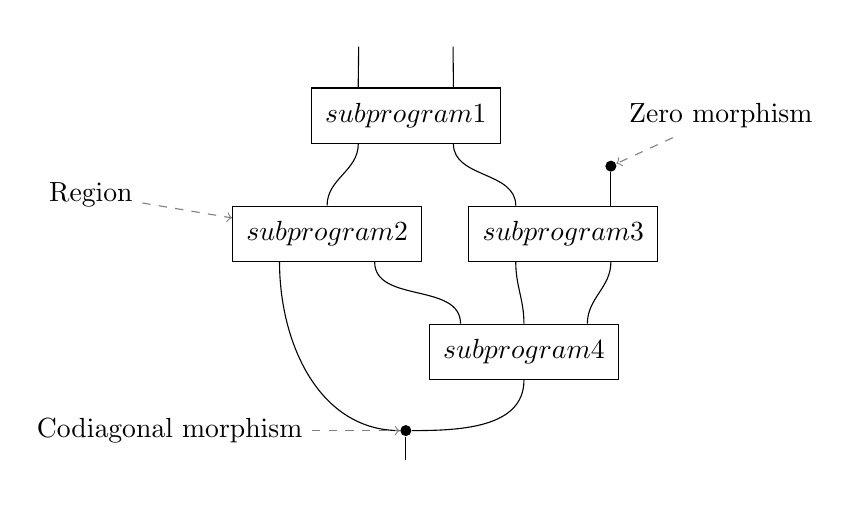
\begin{tikzpicture}
    \node[] (S1) at (-0.6, 1) {};
    \node[] (S2) at (0.6, 1) {};
    \node[box=2/0/2/0] (A) at (0, 0) {\text{subprogram 1}};
    \node[box=1/0/2/0] (B) at (-1, -1.5) {\text{subprogram 2}};
    \node[box=2/0/2/0] (C) at (2, -1.5) {\text{subprogram 3}};
    \node[box=3/0/1/0] (D) at (1.5, -3) {\text{subprogram 4}};
    \node[dot] (zero) at ($(C.north.2)+(0, 0.5)$) {};
    \node[dot] (codiag) at (0, -4) {};
    \node[] (end) at (0, -4.5) {};
    \wires{
      S1 = { south = A.north.1 },
      S2 = { south = A.north.2 },
      A = { south.1 = B.north.1, south.2 = C.north.1 },
      B = { south.1 = codiag.west, south.2 = D.north.1 },
      C = { south.1 = D.north.2, south.2 = D.north.3 },
      D = { south = codiag.east },
      zero = { south = C.north.2 },
      codiag = { south = end.north }
    }{}

    \node[] (zerolabel) at (4, 0) {Zero morphism};
    \node[] (regionlabel) at (-4, -1) {Region};
    \node[] (codiaglabel) at (-3, -4) {Codiagonal morphism};

    \draw[gray, dashed, ->] (zerolabel) to (zero);
    \draw[gray, dashed, ->] (regionlabel) to (B);
    \draw[gray, dashed, ->] (codiaglabel) to (codiag);
  \end{tikzpicture}
  \caption{
    A string diagram using the coproduct as symmetric monoidal structure, interpreted as a CFG
  }
  \label{fig:coproduct-string-diagrams}
  \Description{A string diagram using the coproduct as symmetric monoidal structure, showing how to
  draw the codiagonal morphism and zero morphism, as well as showing what the analogue to a
  subprogram and region might look like.}
\end{figure}

The power of string diagrams comes from the fact that many syntactically distinct ways to write
equal values are obviously graphically equivalent by \emph{isotopy}: essentially, moving boxes and
wires around. String diagrams also give us an elegant way to represent and reason about Elgot
structures. It turns out that \todo{cite Hyland and Hasegawa} Elgot structures induce a \emph{trace}
on the coproduct: given $f : A + C \to B + C$, we can define 
\begin{equation}
  \ms{Tr}_{A, B}^C(f) 
  = \iota_l ; [f ; B + \iota_r]^\dagger 
  = \iota_l ; f ; [\ms{id}, (\iota_l;f)^\dagger] : A \to B
\end{equation}
Since this satisfies the axioms of a trace over a symmetric monoidal category, we can draw it, and
therefore the Elgot operator, as in Figure~\ref{fig:elgot-string-diagrams}. Continuing with the
control-flow diagram analogy, such traces can be interpreted as \emph{loops}, with the Elgot axioms,
now drawn as diagrams in Figure~\todo{this}, all following by geometric manipulation except for
fixpoint (Figure~\todo{this}).

\begin{figure}
  \begin{subfigure}{0.5\textwidth}
    \centering
    \begin{tikzpicture}
      \node[] (Atrf) at (0, 2) {$A$};
      \node[box] (trf) at (0, 0) {\ms{Tr}_{A, B}^C(f)};
      \node[] (Btrf) at (0, -2) {$B$};
      \node[] (eq) at (2, 0) {=};
      \node[] (A) at (3.5, 2) {$A$};
      \node[box=2/0/2/0] (f) at (3.5, 0) {\quad f \quad};
      \node[] (B) at (3.5, -2) {$B$};
      \coordinate[label=right:$C$] (C) at (4.9, 0) {};
      \coordinate[] (cup) at (4.5, -1) {};
      \coordinate[] (cap) at (4.5, 1) {};
      \wires{
        Atrf = { south = trf.north },
        trf  = { south = Btrf },
        A    = { south = f.north.1 },
        f    = { south.1 = B, south.2 = cup.west },
        cap  = { west = f.north.2, east = C.north },
        C    = { south = cup.east },
      }{}
    \end{tikzpicture}
    \caption{The trace of $f : A + C \to B + C$}
  \end{subfigure}%
  \begin{subfigure}{0.5\textwidth}
    \centering
    \begin{tikzpicture}
      \node[] (Atrf) at (0, 2) {$A$};
      \node[box] (trf) at (0, 0) {f^\dagger};
      \node[] (Btrf) at (0, -2) {$B$};
      \node[] (eq) at (1.5, 0) {=};
      \node[] (A) at (3, 2) {$A$};
      \node[box=1/0/2/0] (f) at (3, 0) {\quad f \quad};
      \node[] (B) at (3, -2) {$B$};
      \node[dot] (codiag) at (3, 1) {};
      \coordinate[label=right:$C$] (C) at (4.4, 0) {};
      \coordinate[] (cup) at (4, -1) {};
      \coordinate[] (cap) at (4, 1) {};
      \wires{
        Atrf    = { south = trf.north },
        trf     = { south = Btrf },
        A       = { south = codiag.north },
        f       = { south.1 = B, south.2 = cup.west },
        codiag  = { south = f.north, east = C.north },
        C       = { south = cup.east },
      }{}
    \end{tikzpicture}
    \caption{
      The fixpoint of $f : A \to B + A$
    }
  \end{subfigure}
  \caption{Representations of the coproduct trace and Elgot structure as string diagrams}
  \label{fig:elgot-string-diagrams}
  \Description{Representations of the coproduct trace and Elgot structure as string diagrams}
\end{figure}

Unfortunately, unmodified string diagrams do not work for premonoidal categories, and hence for
Freyd categories. The reason is because, since not all morphisms are central, premonoidal categories
do not in general validate \emph{sliding}. However, this is easy enough to fix: we can postulate a
``state'' wire, drawn in red, which all impure morphisms require as an input and output, as in
Figure~\ref{fig:premonoidal-string-diagram}. Since the state wire linearly threads through all
impure boxes, it establishes a unique order in which they must be executed; this construction is
shown to be sound in \citet{promonad}. Pure morphisms do not have a state wire, so a digram
representing a pure morphism will simply have a red ``stripe'' on the side. This gives us a
convenient way to distinguish between string diagrams using the monodial structure induced by the
coproduct and those using the premonoidal structure induced by the tensor product in a category
having both (such as a distributive premonoidal category): the latter will have a state wire, while
the former will not.

\begin{figure}
  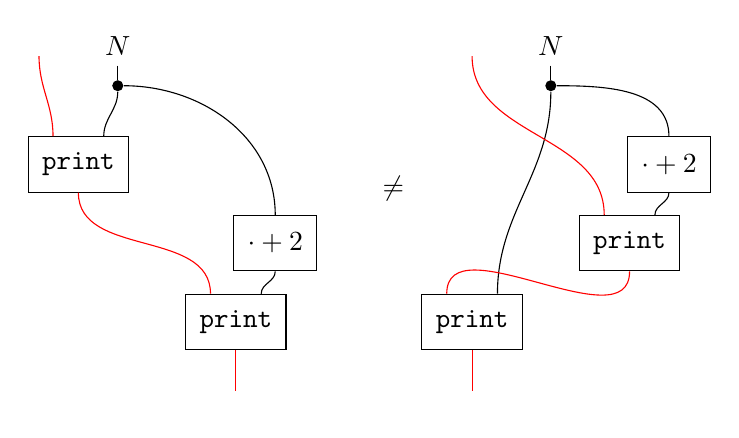
\begin{tikzpicture}
    \node[] (SIa) at (-2.5, 3.5) {};
    \node[] (Na) at (-1.5, 3.5) {$\nats$};
    \node[dot] (codiaga) at (-1.5, 3) {};
    \node[box] (adda) at (0.5, 1) {\cdot + 2};
    \node[box=2/0/1/0] (print1a) at (-2, 2) {\texttt{print}};
    \node[box=2/0/1/0] (print2a) at (0, 0) {\texttt{print}};
    \node[] (SOa) at (0, -1) {};
    \node[] (neq) at (2, 1.7) {$\neq$};
    \node[] (SIb) at (3, 3.5) {};
    \node[] (Nb) at (4, 3.5) {$\nats$};
    \node[dot] (codiagb) at (4, 3) {};
    \node[box=2/0/1/0] (print1b) at (5, 1) {\texttt{print}};
    \node[box] (addb) at (5.5, 2) {\cdot + 2};
    \node[box=2/0/1/0] (print2b) at (3, 0) {\texttt{print}};
    \node[] (SOb) at (3, -1) {};
    \wires{
      Na = { south = codiaga.north },
      codiaga = { south = print1a.north.2, east = adda.north },
      adda = { south = print2a.north.2 },
      Nb = { south = codiagb.north },
      codiagb = { south = print2b.north.2, east = addb.north },
      addb = { south = print1b.north.2 },
    }{}
    \wires[red]{
      SIa = { south = print1a.north.1 },
      print1a = { south = print2a.north.1 },
      print2a = { south = SOa.north },
      SIb = { south = print1b.north.1 },
      print1b = { south = print2b.north.1 },
      print2b = { south = SOb.north },
    }{}
  \end{tikzpicture}
  \caption{
    A string diagram in a premonoidal category, demonstrating the necessity of using a state wire
  }
  \label{fig:premonoidal-string-diagram}
  \Description{A string diagram in a premonoidal category, using a red state wire}
\end{figure}

% One interesting thing this allows us to do is to \emph{nest} coproduct and premonoidal string
% diagrams within each other, by replacing the label in the box with a string diagram, as in
% Figure~\todo{this}. Note that the input wires factor the input (if unlabelled, we should be able to
% determine their type by context), while the output wires are tensored/added together to form the
% output. This will make it a lot easier to express morphisms such as the distributor, which uses both
% the coproduct and premonoidal structure, diagramatically as in Figure~\todo{this}.

\subsection{Semantics}

We now have all the ingredients we need to give a semantics to \isotopessa{} expressions and regions.
In particular, an \isotopessa{} expression model consists of:
\begin{itemize}
  \item A distributive premonoidal category $\mc{C}$
  \item A complete lattice $E$, and a continuous function $\epsilon \mapsto \mc{C}_\epsilon$ from
  $E$ to wide subcategories of $\mc{C}$, such that $\mc{C}_\top = \mc{C}$, and $(\mc{C}, \mc{V} =
  \mc{C}_\bot)$ is a Freyd category. Furthermore, we ask that each $\mc{C}_\epsilon$ is closed under
  tensor products and coproducts, and in particular that injections and (inverse) distributors are
  pure and therefore contained in every $\mc{C}_\epsilon$.
\end{itemize}
If an \isotopessa{} expression model additionally has an Elgot structure, we will refer to it simply
as an \isotopessa{} model.

We will write morphisms $\mc{C}_\epsilon(A, B)$ as $A \to_\epsilon B$, and morphisms $\mc{C}(A, B)$
as $A \to B$. Note that, whenever $\mc{C}$ is a distributive Elgot Freyd category, we can trivially
obtain an \isotopessa{} model by choosing $E = \{\top, \bot\}$; hence, this re-framing does not add
any additional generality, but simplifies bookkeeping. We may also choose $E = \{*\}$ if and only if
$\mc{C}$ is in fact Cartesian.
%
Fixing an \isotopessa{} expression model, we can model types in the obvious manner: 
\begin{itemize}
  \item The unit type $\mb{1}$ is modeled as the monoidal unit $I$
  \item The empty type $\mb{0}$ is modeled as the initial object $\mb{0}$
  \item Products $A \otimes B$ are modeled as tensor products $\dnt{A} \otimes \dnt{B}$
  \item Sum types $A + B$ are modeled as coproducts $\dnt{A} + \dnt{B}$
\end{itemize}
We'll say an \isotopessa{} model \emph{interprets} a signature $(\mc{T}, \mc{I})$ if we have
\begin{itemize}
  \item For every base type $X \in \mc{T}$, an object $\dnt{X} : |\mc{C}|$
  \item For every primitive instruction $f \in \mc{I}_\epsilon(A, B)$, a morphism $\dnt{f} : \dnt{A}
  \to_\epsilon \dnt{B}$.
\end{itemize}
This gives us all the ingredients to interpret \emph{contexts} and \emph{label contexts}, which, as
in Figure~\ref{fig:ssa-ty-sem}, we will interpret as tensor products and coproducts of the
denotations of their parameters, respectively.

\begin{figure}
  \begin{align*}
    \boxed{\dnt{A} : |\mc{C}|} \qquad 
    & \dnt{\mb{1}} = I \qquad
      \dnt{A \otimes B} = \dnt{A} \otimes \dnt{B} \qquad
      \dnt{\mb{0}} = \mb{0} \qquad
      \dnt{A + B} = \dnt{A} + \dnt{B} \qquad \\
    \boxed{\dnt{\Gamma} : |\mc{C}|} \qquad
    & \dnt{\cdot} = I \qquad
      \dnt{\Gamma, \thyp{x}{A}{\epsilon}} = \dnt{\Gamma} \otimes \dnt{A} \\
    \boxed{\dnt{\ms{L}} : |\mc{C}|} \qquad
    & \dnt{\cdot} = 0 \qquad
      \dnt{\ms{L}, \lhyp{\ell}{A}} = \dnt{\ms{L}} + \dnt{A} \\
  \end{align*}
  \begin{equation*}
    \boxed{\dnt{\Gamma \leq \Delta} : \dnt{\Gamma} \to_\bot \dnt{\Delta}}
  \end{equation*}
  \begin{gather*}
    \dnt{\cdot \leq \cdot} = \ms{id}_I \qquad
    \dnt{\Gamma, \thyp{x}{A}{\epsilon} \leq \Delta} = \pi_l;\dnt{\Gamma \leq \Delta} \qquad
    \dnt{\Gamma, \thyp{x}{A}{\epsilon} \leq \Delta, \thyp{x}{A}{\epsilon}}
    = \dnt{\Gamma \leq \Delta} \otimes \dnt{A} \\ \\
  \end{gather*}
  \begin{equation*}
    \boxed{\dnt{\ms{L} \leq \ms{K}} : \dnt{\ms{L}} \to_\bot \dnt{\ms{K}}}
  \end{equation*}
  \begin{gather*}
    \dnt{\cdot \leq \cdot} = \ms{id}_{\mb{0}} \qquad
    \dnt{\ms{L} \leq \ms{K}, \lhyp{\ell}{A}} = \dnt{\ms{L} \leq \ms{K}};\iota_\ell \qquad
    \dnt{\ms{L}, \lhyp{\ell}{A} \leq \ms{K}, \lhyp{\ell}{A}}
    = \dnt{\ms{L} \leq \ms{K}} + \dnt{A}
  \end{gather*}
  \caption{Denotational semantics for \isotopessa{} types, contexts, and weakenings}
  \Description{}
  \label{fig:ssa-ty-sem}
\end{figure}

We can now interpret \isotopessa{} expressions $\hasty{\Gamma}{\epsilon}{a}{A}$ over a given
signature in a model intepreting that signature as morphisms $\dnt{\Gamma} \to_\epsilon \dnt{A}$
using the rules in Figure~\ref{fig:ssa-expr-sem}. Up to this point, both our syntax and semantics
are quite standard; in particular:
\begin{itemize}
  \item Variables $x$ are modeled as projections from the appropriate index in the context's
  denotation $\pi_{\Gamma, x} : \dnt{\Gamma} \to_\bot \dnt{A}$
  \item Applications of primitive instructions $f\;a$ are modeled as $\dnt{f}$ precomposed with the
  denotation of $a$. 
  \item Unary \ms{let}-bindings are modeled by:
  \begin{itemize}
    \item Duplicating the context using the diagonal morphism $\Delta_{\dnt{\Gamma}}$
    \item Passing the right copy of the context through $\dnt{\hasty{\Gamma}{\epsilon}{a}{A}}$ to
    get an input of type $\dnt{\Gamma} \otimes \dnt{A} = \dnt{\Gamma, \bhyp{x}{A}}$
    \item Passing the result of this through $\dnt{\hasty{\Gamma, \bhyp{x}{A}}{\epsilon}{b}{B}}$ to get
    the final result of type $\dnt{B}$
  \end{itemize}
  \item Pairs are modeled by passing the result of the diagonal morphism $\Delta_{\dnt{\Gamma}}$ to
   $
   \dnt{\hasty{\Gamma}{\epsilon}{a}{A}} \ltimes \dnt{\hasty{\Gamma}{\epsilon}{b}{B}}
   $
   i.e., first
   passing the left copy through $\dnt{\hasty{\Gamma}{\epsilon}{a}{A}}$ and then the right copy
   through $\dnt{\hasty{\Gamma}{\epsilon}{b}{B}}$. By the axioms of a Freyd category, for pure
   morphisms, this is the same as simply taking the product
   $
    \langle \dnt{\hasty{\Gamma}{\epsilon}{a}{A}}, \dnt{\hasty{\Gamma}{\epsilon}{b}{B}} \rangle
   $.
  \item Binary \ms{let}-bindings are modeled similarly to unary \ms{let}-bindings, except that after
  passing the right copy of the context through $\dnt{\hasty{\Gamma}{\epsilon}{e}{A \otimes B}}$, we
  re-associate $\dnt{\Gamma} \otimes (\dnt{A} \otimes \dnt{B})$ to $(\dnt{\Gamma} \otimes \dnt{A})
  \otimes \dnt{B} = \dnt{\Gamma, \bhyp{x}{A}, \bhyp{y}{B}}$ before passing the entire result through
  $\dnt{\hasty{\Gamma, \bhyp{x}{A}, \bhyp{y}{B}}{\epsilon}{c}{C}}$.
  \item The unit value $()$ is modeled as the terminal morphism $1_{\dnt{\Gamma}}$, while
  $\ms{abort}\;a$ is modeled as the denotation of $a$ postcomposed with the zero morphism 
  $0_{\dnt{A}}$. Injections, similarly, are simply modeled as the appropriate coproduct injections.
  \item A \ms{case}-expression is modeled by
  \begin{itemize}
    \item Duplicating the context using the diagonal morphism $\Delta_{\dnt{\Gamma}}$
    \item Using the right copy of the context to compute the discriminant using
          $\dnt{\hasty{\Gamma}{\epsilon}{e}{A + B}}$
    \item Applying the inverse distributor $\delta^{-1}$ to obtain a coproduct
          $\dnt{\Gamma} \otimes \dnt{A} + \dnt{\Gamma} \otimes \dnt{B}$
    \item Computing $\dnt{\hasty{\Gamma, x: A}{\epsilon}{a}{C}}$ on the right
          branch and $\dnt{\hasty{\Gamma, y: B}{\epsilon}{b}{C}}$ on the left branch
  \end{itemize}
\end{itemize}

\begin{figure}
  \begin{equation*}
    \boxed{\dnt{\hasty{\Gamma}{\epsilon}{a}{A}} : \dnt{\Gamma} \to_\epsilon \dnt{A}}
  \end{equation*}
  \begin{align*}
    \dnt{\hasty{\Gamma}{\epsilon}{x}{A}} &= \pi_{\Gamma, x} \\
    \dnt{\hasty{\Gamma}{\epsilon}{f\;a}{B}} 
      &= \dnt{f} \circ \dnt{\hasty{\Gamma}{\epsilon}{a}{A}} \\
    \dnt{\hasty{\Gamma}{\epsilon}{\letexpr{x}{a}{b}}{B}}
      &= \Delta_{\dnt{\Gamma}}
      ; \dnt{\Gamma} \otimes \dnt{\hasty{\Gamma}{\epsilon}{a}{A}} ;
      \\&\qquad
      \dnt{\hasty{\Gamma, \bhyp{x}{A}}{\epsilon}{b}{B}}
      \\
    \dnt{\hasty{\Gamma}{\epsilon}{(a, b)}{A \otimes B}} 
      &= \Delta_{\dnt{\Gamma}}
      ; \dnt{\hasty{\Gamma}{\epsilon}{a}{A}} \ltimes \dnt{\hasty{\Gamma}{\epsilon}{b}{B}}
      % ; \dnt{\hasty{\Gamma}{\epsilon}{a}{A}} \otimes \dnt{\Gamma} 
      % ; \dnt{A} \otimes \dnt{\hasty{\Gamma}{\epsilon}{b}{B}}
      \\
    \dnt{\hasty{\Gamma}{\epsilon}{\letexpr{(x, y)}{e}{c}}{C}}
      &= \Delta_{\dnt{\Gamma}}
      ; \dnt{\Gamma} \otimes \dnt{\hasty{\Gamma}{\epsilon}{e}{A \otimes B}} ; \alpha;
      \\&\qquad
      \dnt{\hasty{\Gamma, \bhyp{x}{A}, \bhyp{y}{B}}{\epsilon}{c}{C}}
      \\
    \dnt{\hasty{\Gamma}{\epsilon}{()}{\mb{1}}} &= 1_{\dnt{\Gamma}} \\
    \dnt{\hasty{\Gamma}{\epsilon}{\linl{a}}{A + B}}
      &= \dnt{\hasty{\Gamma}{\epsilon}{a}{A}} ; \iota_l \\
    \dnt{\hasty{\Gamma}{\epsilon}{\linr{b}}{A + B}}
      &= \dnt{\hasty{\Gamma}{\epsilon}{b}{B}} ; \iota_r \\
    \dnt{\hasty{\Gamma}{\epsilon}{\caseexpr{e}{x}{a}{y}{b}}{C}}
      &= \dnt{\hasty{\Gamma}{\epsilon}{e}{A + B}}
      ; \\& \qquad
      \dnt{\hasty{\Gamma, \bhyp{x}{A}}{\epsilon}{a}{A}}
      + \dnt{\hasty{\Gamma, \bhyp{y}{B}}{\epsilon}{b}{B}}
      \\
    \dnt{\hasty{\Gamma}{\epsilon}{\labort{a}}{A}} 
      &= \dnt{\hasty{\Gamma}{\epsilon}{a}{\mb{0}}} ; 0_{\dnt{A}}
  \end{align*}
  \begin{equation*}
    \text{where} \quad \boxed{\pi_{\Gamma, x} : \dnt{\Gamma} \to_\bot \dnt{A}} \qquad
    \pi_{(\Gamma, x : A), x} = \pi_r \qquad
    \pi_{(\Gamma, y : B), x} = \pi_l ; \pi_{\Gamma, x}
  \end{equation*}
  \caption{Denotational semantics for \isotopessa{} expressions}
  \Description{Denotational semantics for isotope-SSA expressions}
  \label{fig:ssa-expr-sem}
\end{figure}

Similarly, if we in fact have an \isotopessa{} model, we can interpret \isotopessa{} regions
$\haslb{\Gamma}{r}{\ms{L}}$ as morphisms $\dnt{\Gamma} \to \dnt{\ms{L}}$; note that we don't assume
anything about the effect of these morphisms. As $\ms{L}$ is a coproduct, we can view the result
object of a region $r$ as encoding both \emph{data} and \emph{control-flow} information. In
particular, we interpret a branch $\brb{\ell}{a}$ as simply the injection of the (pure) expression
$\hasty{\Gamma}{\bot}{a}{A}$, our \emph{data}, into the element of the coproduct corresponding to
$\ell$, which encodes the point in control-flow the rest of the program should jump to next. This is
in contrst to \emph{expressions}, which purely encode data, with no particular instructions on how
to use it afterwards. Our interpretation of \ms{let}-statements and \ms{case}-statements, given in
Figure~\ref{fig:ssa-reg-sem}, is exactly the same as that of the corresponding expressions.

Finally, we come to the interpretation of \ms{where}-blocks, which is where Elgot structure comes
in. Since the semantics for \ms{where} blocks has a lot of moving parts, it makes sense to break it
down ``imperatively" as follows:
\begin{itemize}
  \item First, we split the context using the diagonal morphism $\Delta_{\dnt{\Gamma}}$
  \item Then, using the right copy of the context, we execute the program
  $\dnt{\haslb{\Gamma}{r}{\ms{L}, (\lhyp{\ell_i}{A_i},)_i}}$, and reassociate the result using
  $\alpha^+$ to get to $\dnt{\ms{L}} + \Sigma_i\dnt{A_i}$
  \item We apply the inverse distributor $\delta^{-1}$ to get to the coproduct $\dnt{\Gamma} \otimes
  \dnt{\ms{L}} + \dnt{\Gamma} \otimes \Sigma_i \dnt{A_i}$
  \item In the left ($\dnt{\Gamma} \otimes \dnt{\ms{L}}$) branch, we discard $\dnt{\Gamma}$ and
  return immediately
  \item In the right ($\dnt{\Gamma} \otimes \Sigma_i \dnt{A_i}$) branch, we enter a loop
  (represented by the Elgot iteration operator), in which we:
  \item Apply the inverse distributor $\delta^{-1}_{\Sigma}$ to get to 
        $\Sigma_i \dnt{\Gamma} \otimes \dnt{A_i}$
  \item For each branch $i$ in the sum, we:
  \begin{itemize}
    \item Split the context using the diagonal morphism $\Delta_{\dnt{\Gamma}}$, leaving the
    argument alone; then reassociate to get to $\dnt{\Gamma} \otimes (\dnt{\Gamma} \otimes \dnt{A})$
    \item Use the right component to execute the program $\dnt{\haslb{\Gamma,
    \bhyp{x_i}{A_i}}{t_i}{\ms{L}, (\lhyp{\ell_j}{A_j},)_j}}$, then re-associate the result in the
    coproduct, reaching $\dnt{\Gamma} \otimes (\dnt{\ms{L}} + \Sigma_i\dnt{A_i})$
    \item Apply the inverse distributor $\delta^{-1}$ to get to 
      $\dnt{\Gamma} \otimes \dnt{\ms{L}} + \dnt{\Gamma} \otimes \Sigma_i\dnt{A_i}$
  \end{itemize}
  \item In the left ($\dnt{\Gamma} \otimes \dnt{\ms{L}}$) case, we discard $\dnt{\Gamma}$ and break
  out of the loop
  \item In the right ($\dnt{\Gamma} \otimes \Sigma_i\dnt{A_i}$) case, we return to the beginning
  of the loop for another iteration
\end{itemize}

\begin{figure}
  \begin{equation*}
    \boxed{\dnt{\haslb{\Gamma}{r}{\ms{L}}} : \dnt{\Gamma} \to \dnt{\ms{L}}}
  \end{equation*}
  \begin{align*}
    \dnt{\haslb{\Gamma}{\brb{\ell}{a}}{\ms{L}}} 
      &= \dnt{\hasty{\Gamma}{\bot}{a}{A}} ; \iota_{\ms{L}, \ell}
      \\
    \dnt{\haslb{\Gamma}{\letstmt{x}{a}{r}}{\ms{L}}}
      &= \Delta_{\dnt{\Gamma}}
      ; \dnt{\Gamma} \otimes \dnt{\hasty{\Gamma}{\epsilon}{a}{A}}
      ; \dnt{\haslb{\Gamma, \bhyp{x}{A}}{r}{\ms{L}}} 
      \\
    \dnt{\haslb{\Gamma}{\letstmt{(x, y)}{e}{r}}{\ms{L}}}
      &= \Delta_{\dnt{\Gamma}}
      ; \dnt{\Gamma} \otimes \dnt{\hasty{\Gamma}{\epsilon}{e}{A \otimes B}}
      ; \dnt{\haslb{\Gamma, \bhyp{x}{A}, \bhyp{y}{B}}{r}{\ms{L}}} 
      \\ 
    \dnt{\haslb{\Gamma}{\casestmt{e}{x}{r}{y}{s}}{\ms{L}}}
      &= \Delta_{\dnt{\Gamma}}
      ; \dnt{\Gamma} \otimes \dnt{\hasty{\Gamma}{\epsilon}{e}{A + B}}
      ; \delta^{-1} ;
      \\&\quad\;
      \dnt{\haslb{\Gamma, \bhyp{x}{A}}{r}{\ms{L}}}
      + \dnt{\haslb{\Gamma, \bhyp{y}{B}}{s}{\ms{L}}}
      \\
    \dnt{\haslb{\Gamma}{\where{r}{(\wbranch{\ell_i}{x_i}{t_i},)_i}}{\ms{L}}}
      &=  
      \Delta_{\dnt{\Gamma}}
      ; \dnt{\Gamma} \otimes (\dnt{\haslb{\Gamma}{r}{\ms{L}, (\lhyp{\ell_i}{A_i},)_i}} 
      ; \alpha^+_{\dnt{L} + \Sigma_i \dnt{A_i}} ; \delta^{-1} ; 
      \\ &\quad [\pi_r, 
        (\delta^{-1}_{\Sigma} ;
          [ 
            \Delta_{\dnt{\Gamma}} \otimes \dnt{A_i} ; \alpha ;
      \\ & \qquad
            \dnt{\Gamma} \otimes 
            \dnt{\haslb{\Gamma, \bhyp{x_i}{A_i}}{t_i}{\ms{L}, (\lhyp{\ell_j}{A_j},)_j}}
          ]_i ; \alpha^+_{\dnt{L} + \Sigma_i A_i} ; \delta^{-1}
        )^\dagger ; \pi_r
      \\ & \quad ]
  \end{align*}
  \caption{Denotational semantics for \isotopessa{} regions}
  \Description{Denotational semantics for isotope-SSA regions}
  \label{fig:ssa-reg-sem}
\end{figure}

\subsection{Metatheory}

We can now begin to state the metatheoretic properties of our denotational semantics. We begin with
weakening: as shown in Figure~\ref{fig:ssa-ty-sem}, weakenings are modeled, essentially, as
projections from a larger product $\dnt{\Gamma}$ to a smaller product $\dnt{\Delta}$, while
label-weakenings are modeled as injections from a smaller coproduct $\dnt{\ms{L}}$ to a larger
coproduct $\dnt{\ms{K}}$; in particular, in both cases, the morphisms are pure.  A simple induction
can then be used to derive the following weakening lemmas:
\begin{lemma}[(Label) Weakening]
  Given $\Gamma \leq \Gamma'$ and $\ms{L}' \leq \ms{L}$, $\ms{K}' \leq \ms{K}$, we have
  \begin{enumerate}[label=(\alph*)]
    \item $\dnt{\Gamma \leq \Delta} = \dnt{\Gamma \leq \Gamma'};\dnt{\Gamma' \leq \Delta}$
    \item $\dnt{\ms{L}' \leq \ms{K}} = \dnt{\ms{L}' \leq \ms{L}};\dnt{\ms{L} \leq \ms{K}}$
    \item $\dnt{\hasty{\Gamma}{\epsilon}{a}{A}} 
      = \dnt{\Gamma \leq \Gamma'};\dnt{\hasty{\Gamma'}{\epsilon}{a}{A}}$
    \item $\dnt{\haslb{\Gamma}{r}{\ms{L}}}
      = \dnt{\Gamma \leq \Gamma'}
      ; \dnt{\haslb{\Gamma'}{r}{\ms{L}'}}
      ; \dnt{\ms{L}' \leq \ms{L}}$
    \item $\dnt{\issubst{\gamma}{\Gamma}{\Delta}}
      = \dnt{\Gamma \leq \Gamma'};\dnt{\issubst{\gamma}{\Gamma'}{\Delta}}$
    \item $\dnt{\lbsubst{\Gamma}{\sigma}{\ms{L}}{\ms{K}}}
      = \dnt{\Gamma \leq \Gamma'} \otimes \dnt{\ms{L}}
      ; \dnt{\lbsubst{\Gamma}{\sigma}{\ms{L}}{\ms{K}'}}
      ; \dnt{\ms{K}' \leq \ms{K}}
      $
  \end{enumerate}
\end{lemma}

Our first proper semantic theorem is that \emph{rewriting} is sound: if two (potentially impure!)
substitutions have pointwise equal semantics, then substituting by either yields a result with
the same semantics. That is, value-substitution is a well-defined operation when quotienting by the
semantics, or, more formally:

\begin{theorem}[Soundness (Rewriting)]
  Given substitutions $\issubst{\gamma, \gamma'}{\Gamma}{\Delta}$ such that, for all 
  $\thyp{x}{A}{\epsilon} \in \Delta$, $\dnt{\hasty{\Gamma}{\epsilon}{\gamma\;x}{A}} =
  \dnt{\hasty{\Gamma}{\epsilon}{\gamma'\;x}{A}}$, we have
  \begin{enumerate}[label=(\alph*)]
    \item Given $\hasty{\Delta}{\epsilon}{a}{A}$, 
      $\dnt{\hasty{\Gamma}{\epsilon}{[\gamma]a}{A}} = \dnt{\hasty{\Gamma}{\epsilon}{[\gamma']a}{A}}$
    \item Given $\issubst{\rho}{\Delta}{\Xi}$, $\dnt{\issubst{[\gamma]\rho}{\Gamma}{\Xi}} =
      \dnt{\issubst{[\gamma']\rho}{\Gamma}{\Xi}}$
    \item Given $\haslb{\Delta}{r}{\ms{L}}$, $\dnt{\haslb{\Gamma}{[\gamma]r}{\ms{L}}} =
      \dnt{\haslb{\Gamma}{[\gamma']r}{\ms{L}}}$
    \item Given $\lbsubst{\rho}{\Delta}{\ms{L}}{\ms{K}}$,
      $\dnt{\lbsubst{\Gamma}{[\gamma]\rho}{\ms{L}}{\ms{K}}} =
      \dnt{\lbsubst{\Gamma}{[\gamma']\rho}{\ms{L}}{\ms{K}}}$ 
  \end{enumerate}
  \label{thm:rewriting}
\end{theorem}

This result allows us to safely perform peephole rewrites which we can indepedently prove
semantically valid, including on potentially impure operations. However, for pure substitutions, it
is possible to relate the semantics of the substituted term to the original more precisely. By
\emph{pure} substitutions, we mean substitutions which do not replace variables with impure terms.
More precisely, we can define the \emph{effect} of a context using the lattice structure on effects
as follows
\begin{equation}
  \ms{eff}(\cdot) = \bot \qquad 
  \ms{eff}(\Gamma, \thyp{x}{A}{\epsilon}) = \ms{eff}(\Gamma) \sqcup \epsilon
\end{equation}
We can now give a denotational semantics to substitutions in which a substitution
$\issubst{\gamma}{\Gamma}{\Delta}$ is interpreted as a morphism from $\dnt{\Gamma}$ to
$\dnt{\Delta}$ with effect $\leq \ms{eff}(\Delta)$, as in Figure~\ref{fig:ssa-subst-sem}. A
substitution is \emph{pure} if its effect is $\bot$, which in particular is the case if
$\ms{eff}(\Delta) = \bot$. We can now state the soundness of variable substitution as follows:
\begin{theorem}[Soundness (Substitution)]
  Given $\dnt{\issubst{\gamma}{\Gamma}{\Delta}} : \dnt{\Gamma} \to_\bot \dnt{\Delta}$ (in
  particular, this is always the case when $\ms{eff}(\Delta) = \bot$), we have that
  \begin{enumerate}[label=(\alph*)]
    \item $\dnt{\hasty{\Gamma}{\epsilon}{[\gamma]a}{A}} 
      = \dnt{\issubst{\gamma}{\Gamma}{\Delta}};\dnt{\hasty{\Delta}{\epsilon}{a}{A}}$
    \item $\dnt{\haslb{\Gamma}{[\gamma]r}{\ms{L}}}
      = \dnt{\issubst{\gamma}{\Gamma}{\Delta}};\dnt{\haslb{\Delta}{r}{\ms{L}}}$
    \item $\dnt{\issubst{[\gamma]\rho}{\Delta}{\Xi}}
      = \dnt{\issubst{\gamma}{\Gamma}{\Delta}};\dnt{\issubst{\rho}{\Delta}{\Xi}}$
    \item $\dnt{\lbsubst{\Gamma}{[\gamma]\sigma}{\ms{L}}{\ms{K}}}
      = \dnt{\issubst{\gamma}{\Gamma}{\Delta}};\dnt{\lbsubst{\Delta}{\sigma}{\ms{L}}{\ms{K}}}$
  \end{enumerate}
  \label{thm:subst-sound}
\end{theorem}
In particular, this implies that, when $\gamma$ is pure, the semantics of substitution composition
$[\gamma]\rho$is just composition of the denotations of $\gamma, \rho$; note in general that this is
\emph{not} true in general if only the $\rho$ is pure, as can trivially be seen from the example
\(\gamma = x \mapsto \ms{print}; x\), \(\rho = x \mapsto ()\). Note also that we can derive
rewriting (Theorem~\ref{thm:rewriting}) for pure substitutions from soundness of substitution, but
not vice versa; however, rewriting also covers \emph{impure} substitutions; this is similar to the
distinction between \emph{uniformity} (which only holds for pure operations) and \emph{dinaturality}
(which holds in general, but has a more restricted form).

\begin{figure}
  \begin{equation*}
    \boxed{\dnt{\issubst{\gamma}{\Gamma}{\Delta}} 
      : \dnt{\Gamma} \to_{\ms{eff}(\Delta)} \dnt{\Delta}}
  \end{equation*}
  \begin{gather*}
    \dnt{\issubst{\cdot}{\Gamma}{\cdot}} = \tmor{\dnt{\Gamma}}
    \qquad
    \dnt{\issubst{\gamma, x \mapsto e}{\Gamma}{\Delta, \thyp{x}{A}{\epsilon}}}
    = \dmor{\dnt{\Gamma}};\dnt{\issubst{\gamma}{\Gamma}{\Delta}} 
      \otimes \dnt{\hasty{\Gamma}{\epsilon}{e}{A}}
  \end{gather*}
  \begin{equation*}
    \boxed{\dnt{\lbsubst{\Gamma}{\kappa}{\ms{L}}{\ms{K}}} 
      : \dnt{\Gamma} \otimes \dnt{\ms{L}} \to \dnt{\ms{K}}}
  \end{equation*}
  \begin{gather*}
    \dnt{\lbsubst{\Gamma}{\cdot}{\cdot}{\ms{K}}} 
      = \tmor{\dnt{\Gamma}} \otimes \mb{0}; \lambda; 0_{\ms{K}}
    \\
    \dnt{\lbsubst{\kappa, \ell(x) \mapsto r}{\Gamma}{\ms{L}, \ell(A)}{\ms{K}}}
      = \delta ; [
      \dnt{\lbsubst{\kappa}{\Gamma}{\ms{L}}{\ms{K}}}, 
      \dnt{\haslb{\Gamma, \bhyp{x}{A}}{r}{\ms{K}}}
    ]
  \end{gather*}
  \caption{Denotational semantics for \isotopessa{} (label) substitutions}
  \Description{}
  \label{fig:ssa-subst-sem} 
\end{figure}

We can now move on to stating the metatheoretic properties of label-substitutions, which,
thankfully, turn out to be a little bit simpler. In particular, in Figure~\ref{fig:ssa-subst-sem},
we interpret label substitutions $\lbsubst{\Gamma}{\sigma}{\ms{L}}{\ms{K}}$ as morphisms taking
a copy of the context $\dnt{\Gamma}$ and an element of the coproduct $\dnt{\ms{L}}$ to an element
of the coproduct $\dnt{\ms{K}}$, with an arbitrary effect. Label substitution is then sound in
general, as stated in the following theorem:
\begin{theorem}[Soundness (Label Substitution)]
  Given $\lbsubst{\Gamma}{\sigma}{\ms{L}}{\ms{K}}$, we have
  \begin{enumerate}[label=(\alph*)]
    \item $\dnt{\haslb{\Gamma}{[\sigma]r}{\ms{K}}}
      = \dmor{\dnt{\Gamma}}
      ;\dnt{\Gamma} \otimes \dnt{\haslb{\Gamma}{r}{\ms{L}}}
      ;\dnt{\lbsubst{\Gamma}{\sigma}{\ms{L}}{\ms{K}}}$
    \item $\dnt{\lbsubst{\Gamma}{[\sigma]\sigma'}{\ms{M}}{\ms{K}}}
      = \dmor{\dnt{\Gamma}} \otimes \dnt{\ms{L}} ; \alpha
      ; \dnt{\Gamma} \otimes \dnt{\lbsubst{\Gamma}{\sigma'}{\ms{M}}{\ms{L}}}
      ; \dnt{\lbsubst{\Gamma}{\sigma}{\ms{L}}{\ms{K}}}$
  \end{enumerate}
\end{theorem}

\subsection{Equational Theory}

Using the metatheory in the previous section, our goal is now to prove the equational theory given
in Section~\ref{sec:equations} sound with respect to any valid \isotopessa{} model. Stated more
precisely, we have the following:
\begin{theorem}[Soundness (Equational Theory)]
  We have that
  \begin{enumerate}[label=(\alph*)]
    \item $\tmeq{\Gamma}{\epsilon}{a}{a'}{A} \implies 
      \dnt{\hasty{\Gamma}{\epsilon}{a}{A}} = \dnt{\hasty{\Gamma}{\epsilon}{a'}{A}}$
      \label{itm:eqn-sound-expr}
    \item $\lbeq{\Gamma}{r}{r'}{\ms{L}} \implies
      \dnt{\haslb{\Gamma}{r}{\ms{L}}} = \dnt{\haslb{\Gamma}{r'}{\ms{L}}}$
      \label{itm:eqn-sound-region}
    \item $\tmseq{\gamma}{\gamma'}{\Gamma}{\Delta} \implies
      \dnt{\issubst{\gamma}{\Gamma}{\Delta}} = \dnt{\issubst{\gamma'}{\Gamma}{\Delta}}$
      \label{itm:eqn-sound-vsubst}
    \item $\lbseq{\sigma}{\sigma'}{\Gamma}{\ms{L}}{\ms{K}} \implies
      \dnt{\lbsubst{\Gamma}{\sigma}{\ms{L}}{\ms{K}}} 
      = \dnt{\lbsubst{\Gamma}{\sigma'}{\ms{L}}{\ms{K}}}$ 
      \label{itm:eqn-sound-lsubst}
  \end{enumerate}
\end{theorem}
The rest of this section will consist of a sketch of some of the more difficult components of this
proof, in the hope that this will also illuminate the equational theory somewhat. As
\ref{itm:eqn-sound-vsubst} and \ref{itm:eqn-sound-lsubst} follow trivially from
\ref{itm:eqn-sound-expr} and \ref{itm:eqn-sound-region} respectively, we will only cover the latter.

\subsubsection{Expressions}

\begin{proof}
  Our proof is by rule induction on the equational theory. We sketch the cases below:
  \begin{itemize}
    \item \emph{Congruence}: these follow trivially by induction
    \item \brle{initial}, \brle{terminal}: both of these follow trivially from the universal
    property of the initial/terminal object, respectively.
    \item \brle{let$_1$-$\beta$}: this follows from the soundness of substitution; in particular, we
    have that
    \begin{align*}
      \dnt{\hasty{\Gamma}{\epsilon}{[b/x]a}{B}}
      &= \dnt{\issubst{\upg{(x \mapsto b)}}{\Gamma}{\Gamma, \bhyp{x}{A}}}
        ; \dnt{\hasty{\Gamma, \bhyp{x}{A}}{\epsilon}{a}{B}}
      \quad \text{(by Thm. \ref{thm:subst-sound})} \\
      &= \Delta_{\dnt{\Gamma}} 
        ; \dnt{\Gamma} \otimes \dnt{\hasty{\Gamma}{\epsilon}{a}{A}} 
        ; \dnt{\hasty{\Gamma, \bhyp{x}{A}}{\epsilon}{b}{B}} \\
      &= \dnt{\hasty{\Gamma}{\epsilon}{\letexpr{x}{a}{b}}{B}}
    \end{align*}
    \item \brle{let$_1$-case}: follows from the properties of the coproduct; in particular, we have
    that
    \begin{align*}
      & \dnt{\hasty{\Gamma}{\epsilon}{\caseexpr{e}{x}{\letexpr{z}{a}{d}}{y}{\letexpr{z}{b}{d}}}{D}}
      \\ &= \Delta ; \dnt{\Gamma} \otimes \dnt{\hasty{\Gamma}{\epsilon}{e}{A + B}} ; \delta^{-1} ; [
      \\ & \qquad \Delta
            ; \dnt{\Gamma, \bhyp{x}{A}} \otimes \dnt{\hasty{\Gamma, \bhyp{x}{A}}{\epsilon}{a}{C}}
            ; \dnt{\hasty{\Gamma, \bhyp{x}{A}, \bhyp{z}{C}}{\epsilon}{d}{D}}
            ,
      \\  & \qquad \Delta
            ; \dnt{\Gamma, \bhyp{y}{B}} \otimes \dnt{\hasty{\Gamma, \bhyp{y}{B}}{\epsilon}{b}{C}}
            ; \dnt{\hasty{\Gamma, \bhyp{y}{B}, \bhyp{z}{C}}{\epsilon}{d}{D}}
        ]
      \\ &= \Delta ; \dnt{\Gamma} \otimes \dnt{\hasty{\Gamma}{\epsilon}{e}{A + B}} ; \delta^{-1} ; [
      \\ & \qquad \Delta \otimes \dnt{A} ; \alpha
            ; \dnt{\Gamma} \otimes \dnt{\hasty{\Gamma, \bhyp{x}{A}}{\epsilon}{a}{C}}
            ; \dnt{\hasty{\Gamma, \bhyp{z}{C}}{\epsilon}{d}{D}}
            ,
      \\  & \qquad \Delta \otimes \dnt{B} ; \alpha
            ; \dnt{\Gamma} \otimes \dnt{\hasty{\Gamma, \bhyp{y}{B}}{\epsilon}{b}{C}}
            ; \dnt{\hasty{\Gamma, \bhyp{z}{C}}{\epsilon}{d}{D}}
        ]
      \\ &= \Delta ; \dnt{\Gamma} \otimes \dnt{\hasty{\Gamma}{\epsilon}{e}{A + B}} ; \delta^{-1} ; [
      \\ & \qquad \Delta \otimes \dnt{A} ; \alpha
            ; \dnt{\Gamma} \otimes \dnt{\hasty{\Gamma, \bhyp{x}{A}}{\epsilon}{a}{C}}
            ,
      \\  & \qquad \Delta \otimes \dnt{B} ; \alpha
            ; \dnt{\Gamma} \otimes \dnt{\hasty{\Gamma, \bhyp{y}{B}}{\epsilon}{b}{C}}
        ] ; \dnt{\hasty{\Gamma, \bhyp{z}{C}}{\epsilon}{d}{D}}
      \\ &= \Delta ; \Delta \otimes \dnt{\hasty{\Gamma}{\epsilon}{e}{A + B}} ; \delta^{-1} ; 
      \\ & \qquad [
            \alpha ; \dnt{\Gamma} \otimes \dnt{\hasty{\Gamma, \bhyp{x}{A}}{\epsilon}{a}{C}},
            \alpha ; \dnt{\Gamma} \otimes \dnt{\hasty{\Gamma, \bhyp{y}{B}}{\epsilon}{b}{C}}
        ] ; \dnt{\hasty{\Gamma, \bhyp{z}{C}}{\epsilon}{d}{D}}
      \\ &= \Delta ; \Delta \otimes \dnt{\hasty{\Gamma}{\epsilon}{e}{A + B}}  
                   ; \alpha ; \dnt{\Gamma} \otimes (\delta^{-1} ; [
                        \dnt{\hasty{\Gamma, \bhyp{x}{A}}{\epsilon}{a}{C}},
                        \dnt{\hasty{\Gamma, \bhyp{y}{B}}{\epsilon}{b}{C}}
                    ]) ;
      \\ & \qquad \dnt{\hasty{\Gamma, \bhyp{z}{C}}{\epsilon}{d}{D}}
      \\ &= \Delta ; \dnt{\Gamma} \otimes (
                  \Delta ; \dnt{\Gamma} \otimes \dnt{\hasty{\Gamma}{\epsilon}{e}{A + B}} ;
                  \delta^{-1} ; [
                        \dnt{\hasty{\Gamma, \bhyp{x}{A}}{\epsilon}{a}{C}},
                        \dnt{\hasty{\Gamma, \bhyp{y}{B}}{\epsilon}{b}{C}}
                    ]) ;
      \\ & \qquad \dnt{\hasty{\Gamma, \bhyp{z}{C}}{\epsilon}{d}{D}}
      \\ &= \dnt{\hasty{\Gamma}{\epsilon}{\letexpr{z}{(\caseexpr{e}{x}{a}{y}{b})}{d}}{D}}
    \end{align*}
    \item \brle{let$_2$-$\eta$}: follows from the properties of the product; in particular,
    we have that
    \begin{align*}
      &\dnt{\hasty{\Gamma}{\epsilon}{\letexpr{(x, y)}{e}{(x, y)}}{A \otimes B}} \\
      &= \Delta ; \dnt{\Gamma} \otimes \dnt{\hasty{\Gamma}{\epsilon}{e}{A \otimes B}}
                ; \Delta ; 
                \dnt{\hasty{\Gamma, \bhyp{x}{A}, \bhyp{y}{B}}{\bot}{x}{A}} \otimes
                \dnt{\hasty{\Gamma, \bhyp{x}{A}, \bhyp{y}{B}}{\bot}{y}{B}} \\
      &= \Delta ; \dnt{\Gamma} \otimes \dnt{\hasty{\Gamma}{\epsilon}{e}{A \otimes B}}
                ; \Delta ; (\pi_l ; \pi_r) \otimes \pi_r
       = \dnt{\hasty{\Gamma}{\epsilon}{e}{A \otimes B}}
    \end{align*}
    \item \brle{case-inl}: follows from the properties of the coproduct and inverse distributor; in
    particular, we have that
    \begin{align*}
      & \dnt{\hasty{\Gamma}{\epsilon}{\caseexpr{\linl{a}}{x}{c}{y}{d}}{C}}
      \\ &= \Delta 
      ; \dnt{\Gamma} \otimes (\dnt{\hasty{\Gamma}{\epsilon}{a}{A}} ; \iota_l)
      ; \delta^{-1} ; [
        \dnt{\hasty{\Gamma, \bhyp{x}{A}}{\epsilon}{c}{C}}, 
        \dnt{\hasty{\Gamma, \bhyp{y}{B}}{\epsilon}{d}{C}}
      ]
      \\ &= \Delta 
      ; \dnt{\Gamma} \otimes \dnt{\hasty{\Gamma}{\epsilon}{a}{A}}
      ; \iota_l ; [
        \dnt{\hasty{\Gamma, \bhyp{x}{A}}{\epsilon}{c}{C}}, 
        \dnt{\hasty{\Gamma, \bhyp{y}{B}}{\epsilon}{d}{C}}
      ]
      \\ &= \Delta 
      ; \dnt{\Gamma} \otimes \dnt{\hasty{\Gamma}{\epsilon}{a}{A}}
      ; \iota_l ; \dnt{\hasty{\Gamma, \bhyp{x}{A}}{\epsilon}{c}{C}}
      \\ &= \dnt{\hasty{\Gamma}{\epsilon}{\letexpr{x}{a}{c}}{C}}
    \end{align*}
    We can validate \brle{case-inr} analogously
    \item \brle{case-$\eta$}: follows from the properties of the coproduct and distributor; in
    particular, we have
    \begin{align*}
      & \dnt{\hasty{\Gamma}{\epsilon}{\caseexpr{e}{x}{\linl{x}}{y}{\linr{y}}}{A + B}} \\
      &= \Delta ; \dnt{\Gamma} \otimes \dnt{\hasty{\Gamma}{\epsilon}{e}{A + B}} ; \delta^{-1} ; [
        \dnt{\hasty{\Gamma, \bhyp{x}{A}}{\epsilon}{x}{A}};\iota_l,
        \dnt{\hasty{\Gamma, \bhyp{y}{B}}{\epsilon}{y}{B};\iota_r}
      ] \\
      &= \Delta ; \dnt{\Gamma} \otimes \dnt{\hasty{\Gamma}{\epsilon}{e}{A + B}} 
                ; \delta^{-1} ; (\pi_r + \pi_r)
      = \dnt{\hasty{\Gamma}{\epsilon}{e}{A + B}} 
    \end{align*}
  \end{itemize}
  All the other rules can be derived trivially from string diagrammatic reasoning: once all the
  definitions are unfolded, both sides of rule are obviously the same diagram. Some examples are
  pictured in Figure~\todo{this}.
\end{proof}

\subsubsection{Regions}

\begin{proof}
  Our proof is by rule induction on the equational theory. We sketch some of the cases below:
  \begin{itemize}
    \item \brle{let$_1$-$\beta$}, \brle{let$_1$-case}, \brle{case-inl}, \brle{case-inr}: proved
    analgously to the corresponding rules for expressions
    \item \brle{cfg-$\beta_1$}: \todo{this}
    \item \brle{cfg-$\beta_2$}: \todo{this}
    \item \brle{cfg-$\eta$}: \todo{this}
    \item \brle{codiag}: \todo{this}
    \item \brle{uni}: \todo{this}
    \item \brle{dinat}: by label substitution, we have that
    \begin{equation}
      \begin{aligned}
      \dnt{\haslb{\Gamma}{[\sigma^\uparrow]r}{\ms{L}, (\lhyp{\kappa_j}{A_j},)_j}} 
        &= D_r ; \dnt{\ms{L}} + S ; \alpha^+ \\
      \dnt{\haslb{\Gamma, \bhyp{x_i}{A_i}}{[\sigma^\uparrow]t_i}{\ms{L}, (\lhyp{\kappa_j}{A_j},)_j}}
        &= D_{t_i} ; \dnt{\ms{L}} + S ; \alpha^+
      % \\ & = \Delta ; 
      % \dnt{\Gamma} \otimes \dnt{\haslb{\Gamma}{r}{\ms{L}, (\lhyp{\ell_i}{A_i},)_i}} 
      %   \alpha^+ ; \delta^{-1} ; 
      \end{aligned}
    \end{equation}
    where
    \begin{equation}
      \begin{aligned}
        D_r &= \Delta ; 
          \dnt{\Gamma} \otimes (\dnt{\haslb{\Gamma}{r}{\ms{L}, (\lhyp{\ell_i}{A_i},)_i}} ;
            \alpha^+) ; \delta^{-1} ; \pi_r + \dnt{\Gamma} \otimes \Sigma_i \dnt{A_i} 
            \\
        D_{t_i} &= \Delta ; 
          \dnt{\Gamma} \otimes 
            (\dnt{\haslb{\Gamma, \bhyp{x_i}{B_i}}{t_i}{\ms{L}, (\lhyp{\ell_i}{A_i},)_i}} ;
            \alpha^+) ; \delta^{-1} ; \pi_r + \dnt{\Gamma} \otimes \Sigma_i \dnt{A_i} \\
        S &= \dnt{\lbsubst{\Gamma}{\sigma}{(\lhyp{\ell_i}{A_i},)_i}{\lhyp{\kappa_j}{B_j},)_j}}
      \end{aligned}
    \end{equation}
    Hence, we have that
    \begin{equation}
      \begin{aligned}
        & \dnt{\haslb{\Gamma}
        {\where{([\upg{\sigma}]r)}{(\wbranch{\kappa_i}{x_i}{[\upg{\sigma}]t_i},)_i}}
        {\ms{L}}} \\
        &= \Delta ; \dnt{\Gamma} \otimes (D_r ; \dnt{\ms{L}} + S ; \cancel{\alpha^+ ; \alpha^+})
        ; \delta^{-1} ; [\pi_r, (
          \delta^{-1}_\Sigma ; \\ &\qquad [
            \Delta \otimes \dnt{B_i} ; \alpha ; \dnt{\Gamma} \otimes (D_{t_i} ; \dnt{\ms{L}} + S ; 
              \cancel{\alpha^+}) 
          ]_i ; \cancel{\alpha^+} ; \delta^{-1}
        )^{\dagger}; \pi_r] \\
        &= \Delta ; \dnt{\Gamma} \otimes D_r ; \delta^{-1} 
                  ; [\pi_r, \dnt{\Gamma} \otimes S ; (\delta^{-1}_{\Sigma}; 
                  \\ &\qquad [
            \Delta \otimes \dnt{B_i} ; \alpha ; \dnt{\Gamma} \otimes D_{t_i} ; \delta^{-1} ; 
            \dnt{\Gamma} \otimes \dnt{\ms{L}} + \dnt{\Gamma} \otimes S
          ]_i
        )^{\dagger}; \pi_r] \\
        &= \Delta ; \dnt{\Gamma} \otimes D_r ; \delta^{-1} 
                  ; [\pi_r, (\dnt{\Gamma} \otimes S ; \delta^{-1}_{\Sigma}; 
                  [
            \Delta \otimes \dnt{B_i} ; \alpha ; \dnt{\Gamma} \otimes D_{t_i} ; \delta^{-1}
          ]_i
        )^{\dagger}; \pi_r] \\
        &= D_r ; [\dnt{\ms{L}}, 
          \Delta \otimes \Sigma_i \dnt{A_i} 
            ; \alpha ; (\dnt{\Gamma} \otimes S ; \delta^{-1}_{\Sigma}; 
                  [
            \Delta \otimes \dnt{B_i} ; \alpha ; \dnt{\Gamma} \otimes D_{t_i} ; \delta^{-1}
          ]_i
        )^{\dagger}; \pi_r]
      \end{aligned}
    \end{equation}
    Therefore, it suffices to show that
    \begin{equation}
      \begin{aligned}
        & \Delta \otimes \Sigma_i \dnt{A_i} 
            ; \alpha ; (\dnt{\Gamma} \otimes S ; \delta^{-1}_{\Sigma}; 
                  [
            \Delta \otimes \dnt{B_i} ; \alpha ; \dnt{\Gamma} \otimes D_{t_i} ; \delta^{-1}
          ]_i
        )^{\dagger} \\
        &= 
      \end{aligned}
    \end{equation}
    % \begin{equation}
    %   \begin{aligned}
    %   \dnt{\Gamma} \otimes D_r ; \delta^{-1} &= \dnt{\Gamma} \otimes (\Delta ; 
    %     \dnt{\Gamma} \otimes \dnt{\haslb{\Gamma}{r}{\ms{L}, (\lhyp{\ell_i}{A_i},)_i}} ;
    %       \alpha^+ ; \delta^{-1} ; \pi_r + \dnt{\Gamma} \otimes \Sigma_i \dnt{A_i}) ; \delta^{-1} \\
    %       &= ..\dnt{\Gamma} \otimes 
    %   \end{aligned}
    % \end{equation}
  \end{itemize}
  Analogously to for expressions, all the other rules can be derived trivially from string
  diagrammatic reasoning: once all the definitions are unfolded, both sides of rule are obviously
  the same diagram. Some examples are pictured in Figure~\todo{this}.
\end{proof}

\subsection{Completeness}

\label{ssec:completeness}

Now that we've proved the \emph{soundness} of our equational theory, what remains is to prove that
it is \emph{complete}, i.e., that every equation which holds in all \isotopessa{} models can be
derived from it, or, stated more categorically, that our syntax quotiented by the equational theory
forms an initial \isotopessa{} model.
%
Our strategy for doing this is as follows:
\begin{enumerate}
  \item We begin by constructing a category of expressions $\ms{Th}^\otimes(\Gamma)$ and a category
  of regions $\ms{Th}(\Gamma, \ms{L})$ quotiented by our equational theory, and constructing a
  functor from the former to the latter.
  \item We then show that the category of expressions and the category of regions have the structure
  of an \isotopessa{} expression model and \isotopessa{} model, respectively, and hence that
  expressions may be interpreted in the former and both expressions and regions in the latter.

  If we extend the corresponding judgements to the quotient in the obvious manner, it will turn out
  that, for a distinguished variable $\invar$ and label $\outlb$,
  \begin{equation}
    \begin{gathered}
      \hasty{\Gamma, \invar : [\Delta]}{\epsilon}
        {\dnt{\hasty{\Delta}{\epsilon}{a}{A}}_{\ms{Th}^\otimes(\Gamma)}}{A}
        \qquad
      \haslb{\Gamma, \invar : [\Delta]}
        {\dnt{\hasty{\Delta}{\epsilon}{a}{A}}_{\ms{Th}(\Gamma, \ms{L})}}{\ms{L}, \outlb(A)}
        \\
      \haslb{\Gamma, \invar : [\Delta]}
        {\dnt{\haslb{\Delta}{r}{\ms{K}}}_{\ms{Th}(\Gamma, \ms{L})}}{\ms{L}, \outlb([\ms{K}])}
    \end{gathered}
  \end{equation}
  where packing of contexts is defined as in Section~\ref{ssec:records-enums}.
  
  \item Finally, we refine this result to show that
  \begin{equation}
    \begin{gathered}
    \tmeq{\Gamma, \invar : [\Delta]}{\epsilon}
      {\dnt{\hasty{\Delta}{\epsilon}{a}{A}}_{\ms{Th}^\otimes(\Gamma)}}{[a]}{A}
    \\
    \lbeq{\Gamma, \invar : [\Delta]}
      {\dnt{\hasty{\Delta}{\epsilon}{a}{A}}_{\ms{Th}(\Gamma, \ms{L})}}{\ms{ret}\;[a]}{\ms{L}, \outlb(A)}
    \\
    \lbeq{\Gamma, \invar : [\Delta]}
      {\dnt{\haslb{\Delta}{r}{\ms{K}}}_{\ms{Th}(\Gamma, \ms{L})}}{[r]}{\ms{L}, \outlb([\ms{K}])}
    \end{gathered}
  \end{equation}
  where $\ms{ret}\;a := \brb{\outlb}{a}$. Since the packing operator $[\cdot]$ on terms and regions
  from Section~\ref{ssec:records-enums} is injective for pure contexts $\ms{eff}(\Gamma) = \bot$,
  and hence in particular for $\Gamma = \cdot$, $\ms{L} = \cdot$, it follows that in this case the
  category of expressions and the category of regions are the initial distributive \isotopessa{}
  expression model and \isotopessa{} model respectively.
\end{enumerate}

\subsection{Expressions}

We'll begin by going over the entire proof of completeness for expressions, which is the simpler
case. In particular, we may define the category $\ms{Th}_\epsilon^\otimes(\Gamma)$ of expressions
with effect $\epsilon$ as follows:
\begin{itemize}
  \item Objects $|\ms{Th}^\otimes(\Gamma)|$ types $A, B, C$
  \item Morphisms $\ms{Th}^\otimes(\Gamma)_\epsilon(A, B) = \{e \mid \hasty{\Gamma,
    \bhyp{\invar}{A}}{\epsilon}{e}{B}\}$ quotiented by $\tmeq{\Gamma,
    \bhyp{\invar}{A}}{\epsilon}{e}{e'}{B}$
  \item Identity $(\hasty{\Gamma, \bhyp{\invar}{A}}{\bot}{\invar}{A}) \in
  \ms{Th}^\otimes(\Gamma)_\epsilon(A, A)$
  \item Composition $e;e' = (\ms{let}\;\invar = e; e')$, which satisfies
  $$
  \hasty{\Gamma, \bhyp{\invar}{A}}{\epsilon}{e}{B}, \quad
  \hasty{\Gamma, \bhyp{\invar}{B}}{\epsilon}{e'}{C} \qquad \implies \qquad
  \hasty{\Gamma, \bhyp{\invar}{A}}{\epsilon}{e;e'}{C}
  $$
  We may verify that this satisfies the axioms of a category w.r.t. our equational theory
\end{itemize}
In general, the category of expressions $\ms{Th}^\otimes(\Gamma)$ is simply then given by
$\ms{Th}_\top^\otimes(\Gamma)$, which can be viewed as the union of all
$\ms{Th}_\epsilon^\otimes(\Gamma)$.

We now need to equip $\ms{Th}_\epsilon^\otimes(\Gamma)$ with the structure of a premonoidal
category. Obviously, we wish to define the tensor product of types $A$ and $B$ to be simply $A
\otimes B$; we can then begin by defining projections
\begin{equation}
  \hasty{\Gamma, \invar : A \otimes B}{\epsilon}{\pi_l := \ms{let}\;(x, y) = \invar; x}{A} \qquad 
  \hasty{\Gamma, \invar : A \otimes B}{\epsilon}{\ms{let}\;(x, y) = \invar; y}{B}
\end{equation}
By simply using the pair constructor as a cartesian product $\langle a, b \rangle = (a, b)$, this
can be shown to endow $\ms{Th}_\bot^\otimes(\Gamma)$ with the structure of a cartesian category,
allowing us to define the associators, symmetries, and unitors in the natural manner. If we then
define tensor functors
\begin{equation}
  - \otimes X : e \mapsto \ms{let}\;(\invar, x) = \invar; (e ; (\invar, x)) \qquad
  X \otimes - : e \mapsto \ms{let}\;(x, \invar) = \invar; (e ; (x, \invar))
\end{equation}
we find that $\ms{Th}_\epsilon^\otimes(\Gamma)$ and hence in particular $\ms{Th}^\otimes(\Gamma)$ is
endowed with the structure of a Freyd category with pure subcategory $\ms{Th}_\bot^\otimes(\Gamma)$.

Similarly, we wish to show that $A + B$ is the coproduct of $A$ and $B$ in
$\ms{Th}_\epsilon^\otimes(\Gamma)$. Since we already have obvious injection morphisms
\begin{equation}
  \hasty{\Gamma, \invar : A}{\epsilon}{\iota_l := \iota_l\;\invar}{A + B} \qquad
  \hasty{\Gamma, \invar : B}{\epsilon}{\iota_r := \iota_r\;\invar}{A + B}
\end{equation}
we can define the coproduct of morphisms $\hasty{\Gamma, \invar : A}{\epsilon}{a}{C}$ and 
$\hasty{\Gamma, \invar : B}{\epsilon}{b}{C}$ to be simply given by
\begin{equation}
  \hasty{\Gamma, \invar : A + B}{\epsilon}{[a, b] := \caseexpr{\invar}{\invar}{a}{\invar}{b}}{C}
\end{equation}
It is straightforward to verify that this indeed induces a coproduct on
$\ms{Th}_\epsilon^\otimes(\Gamma)$ and hence on $\ms{Th}^\otimes(\Gamma)$
All that remains is to show that $\ms{Th}_\epsilon^\otimes(\Gamma)$ is in fact a \emph{distributive}
Freyd category. To do so, we may define an inverse distributor morphism
\begin{equation}
  \hasty{\Gamma, \invar : A \otimes (B + C)}
    {\epsilon}
    {\delta^{-1} := \ms{let}\;(x, y) = \invar; \caseexpr{y}{z}{\iota_l(x, z)}{z}{\iota_r(x, z)}}
    {A \otimes B + A \otimes C}
\end{equation}
which can easily be shown to be an inverse to the obvious distributor morphism. We may now note that
\begin{equation}
  \dnt{\cdot}_{\ms{Th}^\otimes(\Gamma)} = \mb{1}, \quad
  \dnt{\Delta, \thyp{x}{A}{\epsilon}}_{\ms{Th}^\otimes(\Gamma)} 
    = \dnt{\Delta}_{\ms{Th}^\otimes(\Gamma)} \otimes A
  \qquad \implies \qquad
  \dnt{\Delta}_{\ms{Th}^\otimes(\Gamma)} = [\Gamma]
\end{equation}
Therefore, it follows that, as expected, that
$
  \hasty{\Gamma, \invar : [\Delta]}{\epsilon}
          {\dnt{\hasty{\Delta}{\epsilon}{a}{A}}_{\ms{Th}^\otimes(\Gamma)}}{A}
$
and it remains to show that we in fact have
$$
  \tmeq{\Gamma, \invar : [\Delta]}{\epsilon}
        {\dnt{\hasty{\Delta}{\epsilon}{a}{A}}_{\ms{Th}^\otimes(\Gamma)}}{[a]}{A}
$$
which can be done by a relatively straightforward induction, implying, since $[\cdot]$ is injective
w.r.t. our equational theory for pure contexts, the following theorem:
\begin{theorem}[Completeness (Expressions)]
  We have that, for all pure $\ms{eff}(\Gamma) = \bot$,
  $$
    \tmeq{\Gamma}{\epsilon}{e}{e'}{A} 
    \iff \dnt{\hasty{\Gamma}{\epsilon}{e}{A}}_{\ms{Th}^\otimes(\cdot)} 
         = \dnt{\hasty{\Gamma}{\epsilon}{e'}{A}}_{\ms{Th}^\otimes(\cdot)}
  $$
  In particular, this implies that $\ms{Th}(\cdot)$ is the initial \isotopessa{} expression model
\end{theorem}

\subsection{Regions}

We define the category $\ms{Th}(\Gamma, \ms{L})$ of regions as follows:
\begin{itemize}
  \item Objects $|\ms{Th}(\Gamma, \ms{L})|$ types $A, B, C$
  \item Morphisms $\ms{Th}(\Gamma, \ms{L})(A, B) = 
    \{r \mid \haslb{\Gamma, \bhyp{\invar}{A}}{r}{\ms{L}, \outlb(B)}\}$ 
    quotiented by $\lbeq{\Gamma, \bhyp{\invar}{A}}{r}{r'}{\ms{L}, \outlb(B)}$
  \item Identity $\haslb{\Gamma, \bhyp{\invar}{A}}{\ms{br}\;\ms{ret}\;\invar}{\ms{L}, \outlb(A)}$
    where $\ms{ret}\;a := \brb{\outlb}{a}$
  \item Composition $r;r' = [\upg{(\outlb(\invar) \mapsto r')}]r$
\end{itemize}
In particular, we may view $\ms{ret}$ as an identity-on-objects functor
$\ms{Th}^\otimes_\bot(\Gamma) \to \ms{Th}(\Gamma, \ms{L})$ with action on morphisms given by given
by 
\begin{equation}
  \hasty{\Gamma, \invar : A}{\bot}{e}{B} 
  \qquad \mapsto \qquad 
  \haslb{\Gamma, \invar(A)}{\ms{ret}\;e}{\ms{L}, \outlb(B)}
\end{equation}
We will use this to equip $\ms{Th}(\Gamma, \ms{L})$ with the structure of a Freyd category.
In particular, taking our subcategory of pure morphisms to be the image of $\ms{ret}$ in 
$\ms{Th}(\Gamma, \ms{L})$, we may define the obvious tensor functors
\begin{equation}
  - \otimes X : r \mapsto \ms{let}\;(\invar, x) = \invar; (r ; \ms{ret}\;(\invar, x)) \qquad
  X \otimes - : r \mapsto \ms{let}\;(x, \invar) = \invar; (r ; \ms{ret}\;(x, \invar))
\end{equation}
Our premonoidal structure is then completely described by requiring that $\ms{ret}$ preserves all
relevant structure, i.e., that we have
\begin{equation}
  \alpha = \ms{ret}\;\alpha \qquad
  \lambda = \ms{ret}\;\lambda \qquad
  \rho = \ms{ret}\;\rho \qquad
  \sigma = \ms{ret}\;\sigma \qquad
  \Delta = \ms{ret}\;\Delta
\end{equation}
Just like for expressions, we can write the coproduct of 
$\haslb{\Gamma, \bhyp{\invar}{A}}{s}{\ms{L}, \outlb(C)}$ and
$\haslb{\Gamma, \bhyp{\invar}{B}}{t}{\ms{L}, \outlb(C)}$
in $\ms{Th}(\Gamma, \ms{L})$ as
\begin{equation}
  \haslb{\Gamma, \invar : A + B}{[s, t] 
    := \casestmt{\invar}{\invar}{s}{\invar}{t}}{\ms{L}, \outlb(C)}
\end{equation}
with the obvious injections $\iota_l := \ms{ret}\;\iota_l$ and $\iota_r = \ms{ret}\;\iota_r$. It
turns out that in this case $\ms{ret}$ preserves coproducts as well, and we can therefore easily
conclude that our category is distributive by taking inverse distributor $\delta^{-1} =
\ms{ret}\;\delta^{-1}$.

All that remains now is to take $\ms{Th}(\Gamma, \ms{L})$ from an \isotopessa{} expression model
to an \isotopessa{} model by giving it an Elgot structure. We do so by defining the fixpoint
of a morphism $\haslb{\Gamma, \invar : A}{r}{\ms{L}, \outlb(B + A)}$ as follows:
\begin{equation}
  \haslb{\Gamma, \invar : A}
    {r^\dagger := \where{\ms{br}\;\ms{go}\;\invar}{\wbranch{\ms{go}}{\invar : A}
        {r ; \casestmt{\invar}{x}{\ms{ret}\;x}{y}{\ms{br}\;\ms{go}\;y}}}}
    {\ms{L}, \outlb(B)}
\end{equation}
where $\ms{go}$ is an (arbitrary) fresh label. We can verify this indeed satisfies the axioms of
an Elgot structure through a somewhat tedious calculation. We may now note that
\begin{equation}
  \begin{aligned}
    \dnt{\cdot}_{\ms{Th}(\Gamma, \ms{L})} 
      &= \mb{1}, &
    \dnt{\Delta, \thyp{x}{A}{\epsilon}}_{\ms{Th}(\Gamma, \ms{L})} 
      &= \dnt{\Delta}_{\ms{Th}(\Gamma, \ms{L})} \otimes A
    &\qquad \implies \qquad
    \dnt{\Delta}_{\ms{Th}(\Gamma, \ms{L})} &= [\Gamma] \\
    \dnt{\cdot^+}_{\ms{Th}(\Gamma, \ms{L})} &= \mb{0}, &
    \dnt{\ms{K}, \ell(A)}_{\ms{Th}(\Gamma, \ms{L})} 
      &= \dnt{\ms{K}}_{\ms{Th}(\Gamma, \ms{L})} + A
    &\qquad \implies \qquad
    \dnt{\ms{K}}_{\ms{Th}(\Gamma, \ms{L})} &= [\ms{K}]
  \end{aligned}
\end{equation}
and hence that 
\begin{equation*}
  \haslb{\Gamma, \invar : [\Delta]}
        {\dnt{\hasty{\Delta}{\epsilon}{a}{A}}_{\ms{Th}(\Gamma, \ms{L})}}{\ms{L}, \outlb(A)}
      \qquad
  \haslb{\Gamma, \invar : [\Delta]}
    {\dnt{\haslb{\Delta}{r}{\ms{K}}}_{\ms{Th}(\Gamma, \ms{L})}}{\ms{L}, \outlb([\ms{K}])}
\end{equation*}
as expected. It is relatively easy to derive that
\begin{equation*}
  \lbeq{\Gamma, \invar : [\Delta]}
        {\dnt{\hasty{\Delta}{\epsilon}{a}{A}}_{\ms{Th}(\Gamma, \ms{L})}}
        {\ms{ret}\;[a]}
        {\ms{L}, \outlb(A)}
\end{equation*}
by a relatively straightforward induction. A much more tedious induction is required to prove that
\begin{equation*}
  \lbeq{\Gamma, \invar : [\Delta]}
        {\dnt{\haslb{\Delta}{r}{\ms{K}}}_{\ms{Th}(\Gamma, \ms{L})}}
        {[r]}
        {\ms{L}, \outlb([\ms{K}])}
\end{equation*}
since the case for \ms{where}-statements is particularly complex. However, after this point, we're
essentially done, and can state our completeness theorem as follows:
\begin{theorem}[Completeness (Regions)]
  We have that, for all pure $\ms{eff}(\Gamma) = \bot$,
  $$
    \lbeq{\Gamma}{r}{r'}{\ms{L}} 
    \iff \dnt{\haslb{\Gamma}{r}{\ms{L}}}_{\ms{Th}(\cdot, \cdot)} 
        = \dnt{\haslb{\Gamma}{r'}{\ms{L}}}_{\ms{Th}(\cdot, \cdot)} 
  $$
  In particular, this implies that $\ms{Th}(\cdot, \cdot)$ is the initial \isotopessa{} model.
\end{theorem}

\section{Concrete Models}

\label{sec:concrete}

\subsection{Monads and Monad Transformers}

As previously stated, every strong monad over a CCC, by virtue of providing a
model of higher-order effectful programming, \emph{also} provides a model of
first-order effectful programming, i.e., SSA. In particular, the Kleisli
category of every such strong monad $\ms{T}$ is a premonoidal category and
induces a Freyd category with pure morphisms given by
\begin{equation}
  \ms{C}_{\ms{T}\bot}(A, B) = \{f;\eta_B : A \to \ms{T}B\} 
  \subseteq \ms{C}(A, \ms{T}B) = \ms{C}_{\ms{T}}(A, B)
\end{equation}
It follows that every strong Elgot monad over a CCC with all coproducts is an
\isotopessa{} model (since, in particular, every CCC with coproducts is
distributive). This allows us to very quickly amass a large collection of
\isotopessa{} models from the literature on strong Elgot monads.

Probably the simplest example of an \isotopessa{} model is given by the
\emph{option monad} $\ms{Option}\;A = A + \mb{1}$, with fixpoint operation
$$
  f^\dagger = \ms{some}\;b \quad \text{if} \quad \exists n, f^n\;a = \ms{some}\;(\iota_l\;b)
  \qquad
  f^\dagger = \ms{none} \quad \text{otherwise}
$$
where
$$
  f^0\;a = \ms{some}\;(\iota_r\;a) \qquad
  f^{n + 1}\;a = \ms{bind}\;(f^{n}\;a)\;[(\ms{pure};\iota_l), f] 
$$
This model allows us to interpret potentially divergent but otherwise purely functional programs.
Another very important \isotopessa{} model is generated by the \emph{powerset monad} $\mc{P}$ over
\ms{Set}, which has fixpoint operation
$$
  f^\dagger\;a = \bigcup_n\{b \mid \iota_l\;b \in f^n\;a\}
$$
We can use this monad to interpret \emph{nondeterministic} potentially divergent functional
programs. We can further expand our repertoire of \isotopessa{} models by considering \emph{monad
transformers}, many of which preserve Elgot-ness. For example, if $\ms{T}$ is a strong Elgot over
\ms{Set},
\begin{itemize}
  \item For all types $R$, the \emph{reader transformer}
  $\ms{ReaderT}\;R\;\ms{T}\;A = R \to \ms{T}\;A$ is strong Elgot 
  with monad operations
  \begin{equation}
    \eta\;a = \lambda - . \eta_{\ms{T}}\;a \qquad
    \ms{bind}\;a\;f = \lambda r. \ms{bind}_{\ms{T}}\;(a\;r)\;(\lambda a. f\;a\;r)
  \end{equation}
  and fixpoint
  \begin{equation}
    f^\dagger = \lambda r.(\lambda a. f\;a\;r)^{\dagger_{\ms{T}}} 
  \end{equation}
  \item For all monoids $W$, the \emph{writer transformer}
  $\ms{WriterT}\;W\;\ms{T}\;A = \ms{T}\;(A \times W)$ is strong Elgot 
  with monad operations
  \begin{equation}
    \eta\;a = (\eta_{\ms{T}}\;a, 1) \qquad
    \ms{bind}\;a\;f = \ms{bind}_{\ms{T}}\;a\;(\lambda (a, w). 
      \ms{bind}\;(f\;a)\;(\lambda (b, w') . (b, w \cdot w')))
  \end{equation}
  and fixpoint
  \begin{equation}
    f^\dagger\;a = (
        \lambda (a, w). \ms{bind}_{\ms{T}}\;(f\;a)\;
          (\lambda (b, w') . \eta_{\ms{T}}([(\cdot, w \cdot w'), (\cdot, w \cdot w')]\;b))
      )^{\dagger_{\ms{T}}}
      (a, 1)
  \end{equation}
  \item For all types $S$, the \emph{state transformer}
  $\ms{StateT}\;S\;\ms{T}\;A = S \to \ms{T}(A \times S)$ is strong Elgot 
  with monad operations
  \begin{equation}
    \eta\;a = \lambda s. \eta_{\ms{T}}\;(a, s) \qquad
    \ms{bind}\;a\;f = \lambda s. \ms{bind}_{\ms{T}}\;(a\;s)\;(\lambda (a, s'). f\;a\;s')
  \end{equation}
  and fixpoint
  \begin{equation}
    f^\dagger = \lambda s.(\lambda (a, s'). 
      \ms{bind}_{\ms{T}}\;(f\;a\;s')\;(\lambda (b, s') . 
        \eta_{\ms{T}}([(\cdot, s'), (\cdot, s')]\;b)))^{\dagger_{\ms{T}}}
  \end{equation}
\end{itemize}

One other important source of \isotopessa{} models is via \emph{Elgot submonads}
of monads on \ms{Set}, which we define as follows:
\begin{definition}[Elgot submonad]
  A monad $(\ms{S}, \eta', \mu')$ is a submonad of $(\ms{T}, \eta, \mu)$ if
  $\eta = \eta'$, $\forall A, \ms{S}\;A \subseteq \ms{T}\;A$, and, on the set
  $\ms{S}\;(\ms{S}\;A) \subseteq \ms{T}\;(\ms{T}\;A)$, $\mu = \mu'$. We say
  $\ms{S}$ is \emph{strong Elgot} if $\ms{T}$ is strong Elgot and, for all $f
  \in A \to \ms{S}\;(A + B)$, $f^\dagger \in A \to \ms{S}\;B$ (i.e. the fixpoint
  operation sends the Kleisli category of $\ms{S}$ to itself).
\end{definition}
One useful property this definition has is that the intersection of arbitrarily many (Elgot)
submonads forms an (Elgot) submonad, i.e., the (Elgot) submonads form a complete lattice.

\subsection{Trace Models}

A particularly important class of \isotopessa{} models are what we will call
\emph{trace models}, which can be viewed as programs which either diverge or
produce a result, while also producting (potentially nondeterministic,
potentially infinite) traces of events $\epsilon \in \mc{E}$.

\TODO{naming}

\begin{definition}[(Monoidal) Stream Action]
  A \textit{stream action} $(M, I, \cdot, \Sigma)$ is a set $M$ of \emph{finite
  effects} and set $I$ of \emph{divergent effects} equipped with a binary
  function (``action'') $\cdot : M \times I \to I$ and a function $\Sigma : M^\omega \to I$
  mapping infinite streams of $M$ to an element of $I$ satisfying $\Sigma \sigma
  = \sigma_0 \cdot \Sigma_i \sigma_{i + 1}$, where $\Sigma_i \sigma_i = \Sigma
  (\lambda i. \sigma_i)$. If $M$ is a monoid and $(M, I, \cdot)$ a monoid
  action, in which case we have a \emph{monoidal} stream action
\end{definition}
The most important example of a monoidal stream action is the \emph{free}
monoidal stream action over a set $E$, called the set of \emph{events}, where:
\begin{itemize}
  \item $M = E^*$ is the free monoid over a set of ``events" $\epsilon \in E$, i.e., the
  monoid of finite lists of events
  \item $I = E^{\leq \omega}$ is the set of \textit{potentially} infinite
  streams of events $\epsilon \in E$
  \item $m \cdot i$ is defined in the obvious manner, i.e. by prepending the (finite) list $m$ to
  the (potentially infinite) stream $i$
  \item $\Sigma\;\sigma$ is defined as the supremum $\bigsqcup_it_i$, where $t
  \leq t'$ iff $t$ is a prefix of $t'$, $t_0 = \bot$ (the empty stream), and
  $t_{i + 1} = t_i \cdot \sigma_i$
\end{itemize}
Other important examples include:
\begin{itemize}
  \item The free stream action over a set of events $E$, where $M = E$, $I =
  E^\omega$ (the set of infinite streams of events $\epsilon$), $m \cdot i$ is
  merely prepending $m$ to the stream $i$, and $\Sigma \sigma = \sigma$
  \item The terminal stream action over an arbitrary set $M$, where $I
  = \mb{1}$. This is always a monoidal stream action if $M$ is a monoid
\end{itemize}

\begin{definition}[Trace Monad Transformer]
  Given a monoidal stream action $(M, I, \cdot, \Sigma)$, we can define the \emph{trace
  monad transformer} over $\ms{Set}$ as follows:
  $
  \ms{TraceT}\;\Sigma\;\ms{T}\;A = \ms{T}\;(A \times M + I)
  $
  with monad operations
  $$
    \eta = (\lambda a. \iota_l (a, 0)) ; \eta_{\ms{T}} \qquad
    \ms{bind}\;a\;f 
    = \ms{bind}_{\ms{T}}\;a\;[\lambda (a, m). m \cdot f a, \lambda i. \eta_{\ms{T}}(\iota_r\;i)]
  $$
  This yields a family of useful Elgot monads, including
  \begin{itemize}
    \item $\ms{Traces}?\;\Sigma = \ms{TraceT}\;\Sigma\;\mc{P}$, with the fixpoint of 
    $f : A \to B + A$ given by
    \begin{align}
      f^\dagger\;a &= f^\dagger_\infty\;a \cup \bigcup_n f^\dagger_n\;a 
        \qquad \qquad \text{where} \\
      f^\dagger_n\;a &=
          \{\iota_l\;(b, m) \mid \iota_l(\iota_l\;b, m) \in [\ms{id}_B, f]^n(\iota_r\;a)\}
          \cup \{\iota_r\;i \mid \iota_r\;i \in [\ms{id}_B, f]^n(\iota_r\;a)\} \\
      f^\infty\;a &= \{\iota_r \Sigma \sigma \mid \exists \alpha : A^\omega, 
        \alpha_0 = a \land \forall i, \iota_l\;(\iota_r\;\alpha_{i + 1}, \sigma_i) \in f\;\alpha_i \} 
    \end{align}
    We say a morphism $f : A \to \ms{Traces}?\;\Sigma\;B$ is \emph{total} if all $f\;a$ are
    nonempty, and \emph{deterministic} if all $f\;a$ are subsingletons.
    \item $\ms{Traces}\;\Sigma = \ms{TraceT}\;\Sigma\;\mc{P}^+$, which can be viewed as an Elgot
    submonad of $\ms{Traces}?\;\Sigma$ since the fixpoint of a total function is total
    \item $\ms{Trace}?\;\Sigma = \ms{TraceT}\;\Sigma\;\ms{Option}$, which can be viewed as an Elgot
    submonad of $\ms{Traces}?\;\Sigma$ since the fixpoint of a deterministic function is
    deterministic
    \item $\ms{Trace}\;\Sigma = \ms{TraceT}\;\Sigma\;\ms{Id}$, which can be viewed as an Elgot
    submonad of $\ms{Traces}?\;\Sigma$, and in particular the intersection 
    $\ms{Trace}?\;\Sigma \cap \ms{Traces}\;\Sigma$.
  \end{itemize}
\end{definition}

As a simple, concrete example of type type of model this construction lets us define, consider the
\emph{nondeterministic printing monad}, which is simply defined as \(\ms{Print}\;A \equiv
\ms{Traces}\;\Sigma\), where \(\Sigma: (\ms{byte}^*)^\omega \to \ms{byte}^{\leq \omega}\) denotes
concatenation of bytestrings into a (potentially infinite) bytestream. This gives us us an
\isotopessa{} model supporting effectful instructions \(\ms{print}: \ms{byte}^* \to \mb{1}\) and
\(\ms{nondet}: \mb{1} \to A\) (for \(A\) nonempty), with semantics \(\dnt{\ms{print}} = \lambda
b.\{\iota_0 ((), b)\}\), \(\dnt{\ms{nondet}} = \lambda (). \{\iota_0 (a, []) \mid a \in A\}\).

We can make things a little more interesting by adding a heap to the mix, defining our monad
\(\ms{Comp} = \ms{StateT}\;\ms{Heap}\;\ms{Print}\), where \(\ms{Heap} = \nats \rightharpoonup
\nats\) is simply a partial function with finite support. The Kleisli category of this monad is also
a Freyd category and inherits an Elgot structure from that on \(\ms{Set}_{\ms{Print}}\); we
therefore have an \isotopessa{} model supporting the instructions \(\ms{set}: \nats \times \nats \to
\mb{1}\), \(\ms{get}: \nats \to \nats\), \(\ms{alloc}: \nats \to \nats)\), and \(\ms{free}: \nats
\to \mb{1}\). We can assign semantics to \(\ms{set}\) in the standard fashion, with \(\dnt{\ms{set}}
= \lambda (p, v)\;h. \{\iota_0((), [p \mapsto v]h, [])\}\). \(\ms{get}\) is a bit more tricky, since
it is unclear what to do when we try to access uninitialized memory: one option is simply to return
an arbitrary value, with \(\dnt{\ms{get}} = \lambda p\;h. \{\iota_0(v, h, []) \mid v = h\;p \lor p
\notin h\}\). Finally, \(\dnt{\ms{alloc}} = \lambda v\;h.\{\iota_0\;(p, h', []) \mid h' = h \sqcup p
\mapsto v\}\) simply fills a random empty heap cell with the provided value, returning a pointer to
the cell, while \(\dnt{\ms{free}} = \lambda p\;h. \{\iota_0\;((), h \setminus p, [])\}\).

As we can see, the trace monad is a very powerful tool for quickly constructing families of
\isotopessa{} models, at least for relatively simple side-effects. It turns out, however, that the
same techniques can be used to tackle much more complex side-effects; to demonstrate this, we will
show how to build a simple model of TSO weak memory based on that given in \citet{sparky}.

\subsection{TSO weak memory}

\label{ssec:tso}

To start, we need to construct an appropriate stream action monoid to take our traces over. For
simplicity, we will consider an infinite set of named locations \(x, y, z \in \ms{Loc}\) which are
subject to concurrent modification by all threads via TSO reads, writes, and fences. We begin with
the following definitions:
\begin{definition}[Pomset] 
  A \emph{pomset} \(\alpha\) over a set of actions \(\mc{A}\) with a distinguished null action
  "\emph{tick}" \(\delta \in \mc{A}\) is a \textit{nonempty} partially-ordered \emph{carrier set}
  \(P\) such that every \(p \in P\) has finitely many predecessors equipped with a mapping \(\alpha:
  P \to \mc{A}\). A pomset is \emph{finite} if its carrier set is. We will quotient pomsets over the
  removal of arbitrarily many copies of $\delta$ as long as infinite sets are only equated to other
  infinite pomsets. We will write unordered pomsets using multiset notation, e.g. \(\{a, a, b\}\),
  and linearly ordered pomsets using list notation, e.g. \([a, a, b]\).
\end{definition}
(Finite) pomsets form a monoid under sequential composition \(\alpha;\beta\), which is defined by
the function \([\alpha, \beta]: \ms{trim}(P + Q) \to \mc{A}\), where \(P + Q\) is given the
lexicographic ordering and \(\ms{trim}(R)\) removes all elements of \(R\) with infinitely many
predecessors. They also form a monoid under parallel composition, defining \(\alpha || \beta =
[\alpha, \beta]: P + Q \to \mc{A}\) where \(P + Q\) is given the standard partial ordering (with
elements of \(P\) and \(Q\) incomparable). Note in both cases the monoidal unit is \(\{\delta\}\),
since we only consider nonempty pomsets but allow the removal of finitely many ticks. Given any
partially ordered set \(N\) and a family of pomsets \(\alpha_n\) for \(n \in N\), we can define
their \textit{sum} \(\Sigma_n\alpha_n\) to be given by the function \((n, a) \mapsto \alpha_n\;a:
\ms{trim}(\Sigma_nP_n) \to \mc{A}\), where the dependent product \(\Sigma_nP_n\) is given the
lexicographic order. In particular, choosing \(N = \nats\) makes \(\Sigma:
\ms{Pom}_{\ms{fin}}^\omega \to \ms{Pom}\) into a stream action monoid w.r.t the sequential
composition monoid on finite pomsets. 

We define a \emph{program order pomset} to be a pomset with \(\mc{A}_{\ms{PO}} = \mc{A}_w \cup
\mc{A}_r \cup \{\delta\}\), where \(\mc{A}_r\) consists of \textit{reads} of the form \(x = v\) and
\(\mc{A}_w\) consists of \textit{writes} of the form \(x := v\) for locations \(x\) and values \(v
\in \ms{Word}\). We define the \emph{program order monad} \(\ms{PO}\;A = \ms{Traces}\;\Sigma\;A\),
where \(\Sigma\) is taken as a stream action on finite program order pomsets. This yields an
\isotopessa{} model with support for concurrent read and write operations \(\ms{read}_x:
\mc{I}^\varnothing_0(\mb{1}, \ms{Word})\), \(\ms{write}_x: \mc{I}^\varnothing_0(\ms{Word}, \mb{1})\)
with semantics
\(
  \dnt{\ms{read}_x} = R_x^{\ms{PO}} = \lambda (). \{(v, \{x = v\}) | v \in \ms{Word}\}
\),
\(
  \dnt{\ms{write}_x} = W_x^{\ms{PO}} =  \lambda v. \{((), \{x := v\})\}
\).
The semantics of \(\ms{read}\) in particular give a hint as to how this model works: rather than
tracking the state of the heap, we simply \textit{emit} a pomset of the events that would have be
generated by a given execution (in the case of a read, a read event \(x = v\) whenever the read
returns \(v\), and in the case of a write, the single write event \(x := v\) for a write of \(v\)),
and later post-filter to obtain a set of valid executions. By doing so, our semantics remains
compositional, allowing us to reason about each program fragment individually, while still allowing
other program fragments to perform concurrent operations affecting our potential executions. On that
note, we can define the \textit{parallel execution} of two morphisms as follows:
\begin{equation}
  \begin{aligned}
  f_0 || f_1 = \lambda (a_0, a_1). 
  & \{\iota_0 ((b_0, b_1), \alpha_0 || \alpha_1) 
    \mid \iota_0 (b_i, \alpha_i) \in f_i\;a_i\} 
  \\ & \cup \{\iota_1 (\alpha_0 || \alpha_1) 
      \mid (\iota_0 (b_0, \alpha_0) \in f_0\;a \lor \iota_0\;\alpha_0 \in f_0\;a_0) 
      \land \iota_1 \alpha_1 \in f_1\;a_1\} 
  \\ & \cup \{\iota_1 (\alpha_0 || \alpha_1) 
      \mid \iota_1\;\alpha_0 \in f_0\;a_0 
      \land \iota_0 (a_1, \alpha_1) \in f_1\;a_1\}
    : \ms{Set}_{\ms{PO}}(A \otimes A', B \otimes B')
  \end{aligned}
\end{equation}
It's tempting to try to use this to define a tensor product of morphisms to obtain a monoidal
(rather than preomonoidal) category, but unfortunately, sliding still fails: \((W_x^{\ms{PO}} ||
\ms{id}) ; (\ms{id} || W_y^{\ms{PO}})\) emits the pomset \([x := a, y := b]\), while \((\ms{id} ||
W_y^{\ms{PO}}) ; (W_x^{\ms{PO}} || \ms{id})\) emits the pomset \([y := b, x := a]\). 
% If we did want this behaviour, we'd need to have a significantly more
% sophisticated model of composition which effectively takes nontermination into
% account, which we will leave to future work.

To graduate from sequential consistency to a genuine, if maximally simple, weak memory model, we
introduce \textit{load buffering} of write actions. We will implement TSO ordering by buffering all
our writes, in which case they are only visible to the local thread. On the other hand, read events
will first attempt to read from the buffer, and, if there is no corresponding write in the buffer,
will read an arbitrary value, in both cases pushing an event to the global pomset. At any point, we
may choose to \textit{flush} some of the buffered writes. We introduce the set \(\mc{A}_b =
\{(\bufloc{x} := v)\}\) of \textit{buffer write actions}, where an action \(\bufloc{x} := v\) by a
thread denotes adding a write \(x := v\) to the thread's write buffer. We may then define the set of
TSO actions \(\mc{A}_{\ms{TSO}} = \mc{A}_{\ms{PO}} \cup \mc{A}_b\); a pomset over this set is called
a \emph{TSO pomset}. A buffer will be defined to be a list of write actions \(\ms{Buf} =
\mc{A}_b^*\), which we will interpret as linear pomsets over \(\mc{A}_{\ms{TSO}}\) ordered by index
(with the empty list corresponding to \(\{\delta\}\)). In particular, we define the monad \(\ms{TSO}
= \ms{StateT}\;\ms{Buf}\;(\ms{Trace}\;\Sigma)\), where \(\Sigma\) is taken as a the stream action of
finite TSO pomsets on TSO pomsets. We can view \(\ms{PO}\) as a submonad of this monad.

Given a buffer \(\ms{Buf}\), we can define the result of reads \([\cdot]_x: \ms{Buf} \to \ms{Word}
\sqcup \{\bot\}\) from the buffer by induction to be:
\(
  (L;\{\bufloc{x} := v\})[x] = v,
\),
\(
  (L;\{\bufloc{y} := v\})[x] = L[x]
\),
\(
  [][x] = \bot
\).
Note that writes at the \textit{end} of the buffer are prioritized, since later writes overwrite
earlier ones! 

The semantics of reads and writes can then be given by
\begin{equation}
  \begin{aligned}
  \dnt{\ms{read}_x} = R_x^{\ms{TSO}} 
    &= \ms{pflush};(\lambda ()\;L. \{(v, L, \{x = v\}) \mid L[x] = v \lor L[x] = \bot\});\ms{pflush} 
  \\
  \dnt{\ms{write}_x} = W_x^{\ms{TSO}}
    &= \ms{pflush};(\lambda v\;L. \{(v, (L;\{\bufloc{x} := v\}), \{x := v\})\});\ms{pflush}
  \end{aligned}
\end{equation}
where buffer flushing is implemented via the morphism 
$$
  \ms{pflush}_A = \lambda a\;L. \{(a, R, \alpha) | L = \alpha;R\}
  : \ms{Set}_{\ms{TSO}}(A, A)
$$
(called \(\ms{split}\) in \cite{sparky}). To be able to perform synchronization, we will also need
to introduce a \(\ms{fence}: \mc{I}^\varnothing_0(\mb{1}, \mb{1})\) instruction, which simply causes
all actions before the fence to be observed before any actions after the fence. For \(\ms{TSO}\),
implementing this is as simple as flushing the buffer, i.e., we define
$$
  \dnt{\ms{fence}} = \lambda ()\;L. \{((), [], L;\{\delta\})\}
$$
We can now define the parallel composition of morphisms in a "fork-join" style as follows: we first
flush the buffer completely (i.e., taking it and sticking it at the beginning of our pomset), then
execute \(f\) and \(g\) in parallel with separate buffers, \textit{filtering out executions which
completely flush the buffer}. Since both threads end up with an empty buffer, the resulting joined
buffer is also empty, giving us the following definition:
\begin{equation}
  \begin{aligned}
    f_0 || f_1 = \lambda (a_0, a_1)\;L. 
    & \{\iota_0 ((b_0, b_1), [], L;(\alpha_0 || \alpha_1)) 
      \mid \iota_0 (b_i, [], \alpha_i) \in f_i\;a_i\;[]\} 
    \\ & \cup \{\iota_1 (\alpha_0 || \alpha_1) 
        \mid (\iota_0 (b_0, [], \alpha_0) \in f_0\;a \lor \iota_0\;\alpha_0 \in f_0\;a_0\;[]) 
        \land \iota_1 \alpha_1 \in f_1\;a_1\;[]\} 
    \\ & \cup \{\iota_1 (\alpha_0 || \alpha_1) 
        \mid \iota_1\;\alpha_0 \in f_0\;a_0\;[] 
        \land \iota_0 (a_1, [], \alpha_1) \in f_1\;a_1\;[]\}
    \end{aligned}
\end{equation}

One issue with this model is that our category currently has ``too many'' operations besides the
ones we want: for example, it is a perfectly valid morphism to simply add an event into the buffer
without any flushing. Of course, one thing we could do is consider the smallest Elgot subcategory
generated by the atomic instructions we want to support, such as \(\ms{read}_x\), \(\ms{write}_x\),
and \(\ms{fence}\), which can be a perfectly valid approach, but is somewhat unwieldy. Another
approach, however, is to think about what ``valid'' morphisms might look like in general; this
also has the benefit of letting us write down specifications that may not be trivially implementable
in terms of actual instructions.

There are many potential properties we might want ``valid'' morphisms to have; in general, the less
valid morphisms we admit, the more equations we have to work with when reasoning. One simple
property we might consider is that a ``valid'' morphism must have at least one execution in which
the buffer is completely flushed, regardless of initial state. This is a perfectly reasonable
property to impose, since it ensures that we do not encounter degenerate cases where, for example,
the parallel composition of two processes has an empty trace  set even though both processes have a
nonempty trace set (since neither empties the buffer). We might even want to go a little bit further
and, representing the fact that a buffer flush can happen at any time between instructions, require
that a nondeterministic buffer flush before or after an instruction does not change its semantics,
i.e., that $\ms{pflush}_A ; f ; \ms{pflush}_B = f$. Unfortunately, this does \emph{not} hold for
the identity, since
\begin{equation}
  \ms{pflush} ; \ms{id} ; \ms{pflush} = \ms{pflush} ; \ms{pflush} = \ms{pflush} \neq \ms{id}
\end{equation}
so this would not give us a subcategory. While one possible solution is to simply add the identity
back in (and this would give us a valid subcategory), we have the issue that, for example, morphisms
like the associator and unitor would still be excluded. Instead, we can take into account the fact
that all $\ms{pflush}_A$ are idempotent and define a new category $\ms{PTSO}$ with objects sets and
morphisms of the form
\begin{equation}
  \ms{PTSO}(A, B) = \{\ms{pflush}_A; f; \ms{pflush}_B \mid f \in \ms{Set}_{\ms{TSO}}(A, B)\} 
\end{equation}
In this category, $\ms{pflush}_A$ is the identity on $A$, since
\begin{equation}
  \begin{aligned}
    \ms{pflush}_A ; \ms{pflush}_A; f; \ms{pflush}_B &= \ms{pflush}_A; f; \ms{pflush}_B \\
    \ms{pflush}_A; f; \ms{pflush}_B; \ms{pflush}_B &= \ms{pflush}_A; f; \ms{pflush}_B
  \end{aligned}
\end{equation}
This is especially useful since it frees us from needing to remember to sprinkle $\ms{pflush}$
everywhere when specifying things (and, of course, when that level of control is desired, we can
specify in $\ms{Set}_{\ms{TSO}}$ and then lift to $\ms{PTSO}$).

It turns out that this is a general construction we can do, which gives us another useful way to
build up \isotopessa{} models that can often be quite difficult to express as simply monads.
In particular, we have the following definition
\begin{definition}[Idempotent envelope category]
  Let $\mc{C}$ be a category and $d$ be a family of morphisms for each $A \in |\mc{C}|$ such that
  each $d_A : \mc{C}(A, A)$ is idempotent, i.e., $d_A ; d_A = d_A$. We may then define the
  subsemicategory $\ms{Ide}(\mc{C}, d)$ of $\mc{C}$ to be given by
  \begin{equation}
    \ms{Ide}(\mc{C}, d)(A, B) 
      = \{f \in \mc{C}(A, B) \mid f = d_A ; f ; d_B\}
      = \{d_A ; f ; d_B \mid f \in \mc{C}(A, B)\}
  \end{equation}
  Note that $\ms{Ide}(\mc{C}, d)$ is \emph{not} a subcategory unless $d_A = \ms{id}_A$ for all $A$,
  in which case $\ms{Ide}(\mc{C}, d) = \mc{C}$. However, $\ms{Ide}(\mc{C}, d)$ can be
  \emph{independently} viewed as a category with identity $d_A$ at $A$.
\end{definition}
We have that, if $\mc{C}$ has coproducts and $d_{A + B} = d_A + d_B$, then $\ms{Ide}(\mc{C}, d)$
inherits coproducts from $\mc{C}$ with injections 
\begin{equation}
  \begin{aligned}
    d_A;\iota_l &= \iota_l;d_{A + B} &= d_A;\iota_l;d_{A + B} &\in \ms{Ide}(\mc{C}, d)(A, A + B) 
    \\
    d_B;\iota_r &= \iota_r;d_{A + B} &= d_B;\iota_r;d_{A + B} &\in \ms{Ide}(\mc{C}, d)(B, A + B)
  \end{aligned}
\end{equation}
since, for $f \in \ms{Ide}(\mc{C}, d)(A, C)$, $g \in \ms{Ide}(\mc{C}, d)(A, C)$, we have that
\begin{equation}
  d_{A + B} ; [f, g] ; d_C 
  = d_A + B ; [f, g] ; d_C
  = [d_A ; f ; d_C, d_B ; g ; d_C]
  = [f, g]
\end{equation}
In particular, it follows that $\ms{Ide}_d$ preserves coproducts. If $\mc{C}$ in addition has an
Elgot structure, then $\ms{Ide}(\mc{C}, d)$ also inherits this structure (and therefore $\ms{Ide}_d$
preserves it), as for $f \in \ms{Ide}(\mc{C}, d)(A, B + A)$, we have
\begin{equation}
  f^\dagger 
  = (d_A ; f ; d_B + d_A)^\dagger 
  = (d_A ; f ; d_B + d_A)^\dagger ; d_B
  = d_A ; (f ; d_B + (d_A ; d_A))^\dagger ; d_B
  = d_A ; f^\dagger ; d_B
\end{equation}
On the other hand, if $\mc{C}$ is equipped with a (symmetric) premonoidal structure and we have that
\begin{equation}
  d_{A \otimes B} = d_A \ltimes d_B = d_A \rtimes d_B 
  \qquad d_{A \otimes I} = d_A \otimes I 
  \qquad d_{I \otimes A} = I \otimes d_A
  \label{eqn:d-premonoidal}
\end{equation}
(note that $d$ does \emph{not} have to be central!), it follows that $\ms{Ide}(\mc{C},
d)$ has (symmetric) premonoidal structure as well, with inherited tensor product functors and
associators, unitors, and symmetries given by
\begin{equation}
  \begin{gathered}
    d_{(A \otimes B) \otimes C} ; \alpha_{A, B, C}
    = \alpha_{A, B, C} ; d_{A \otimes (B \otimes C)}
    = d_{(A \otimes B) \otimes C} ; \alpha_{A, B, C} ; d_{A \otimes (B \otimes C)} \\
    d_{A \otimes I} ; \lambda_A = \lambda_A ; d_A = d_{A \otimes I} ; \lambda_A ; d_A \qquad
    d_{I \otimes A} ; \rho_A = \rho_A ; d_A = d_{I \otimes A} ; \rho_A ; d_A \\
    d_{A \otimes B} ; \sigma_{A, B} 
      = \sigma_{A, B} ; d_{B \otimes A} 
      = d_{A \otimes B} ; \sigma_{A, B} ; d_{B \otimes A}
  \end{gathered}
\end{equation} 
respectively. It follows that if $\mc{C}$ is distributive, so is $\ms{Ide}(\mc{C}, d)$, since we can
verify that the distributor $[d_A \otimes (d_B ; \iota_l), d_A \otimes (d_C ; \iota_r)]$ has the
expected inverse
\begin{equation}
  d_{A \otimes (B + C)} ; \delta^{-1} ; d_{(A \otimes B) + (A \otimes C)}
\end{equation}
If we in fact have that $d_{A \otimes B} = A \otimes d_B = d_A \otimes B$ for all $A,
B$ (which implies Equation~\ref{eqn:d-premonoidal}) and $\mc{C}$ is equipped with the structure
of a Freyd category, then so is $\ms{Ide}(\mc{C}, d)$, with projections and diagonal given by
\begin{equation}
  \begin{gathered}
  d_{A \otimes B} ; \pi_l = \pi_l ; d_A = d_{A \otimes B} ; \pi_l ; d_A \qquad
  d_{A \otimes B} ; \pi_r = \pi_r ; d_B = d_{A \otimes B} ; \pi_r ; d_B \\
  d_A ; \Delta = \Delta ; d_{A \otimes A} = d_A ; \Delta ; d_{A \otimes A}
  \end{gathered}
\end{equation}
Hence, it follows that if $\mc{C}$ is an \isotopessa{} (expression) model, $d_A$ is idempotent,
$d_{A + B} = d_A + d_B$, and $d_{A \otimes B} = A \otimes d_B = d_A \otimes B$, then
$\ms{Ide}(\mc{C}, d)$ is an \isotopessa{} (expression) model as well. It turns out that all these
properties hold for $d = \ms{pflush}$, giving us our final categorical model for TSO weak memory,
$\ms{PTSO} = \ms{Ide}(\ms{Set}_{\ms{TSO}}, \ms{pflush})$.

\section{Discussion and Related Work}

\subsection{SSA, FP and IRs}

Static Single Assignment (SSA) form was first introduced as a compiler intermediate representation
by \citet{alpern-ssa-original-88} and \citet{rosen-gvn-1988}, with the goal of facilitating
effective reasoning about program variable equivalence. To perform optimizations like common
subexpression elimination (CSE) effectively, we need to determine which expressions are equal
\emph{at a given point in time}. By transforming the program into SSA form, we introduce unique
variables for each assignment and use $\phi$-nodes to merge variable values at points where control
paths converge. Since each variable then corresponds to a unique value at a specific point in the
program's execution, SSA unlocks the ability to perform \emph{algebraic reasoning} about variable
values over time. As a result, analyses like CSE become a matter of simple algebraic rewriting based
on variable names.

\citet{cytron-ssa-intro-91} provided the first efficient algorithm for converting 3-address code
programs to SSA form using a minimal number of $\phi$-nodes. They observed that a $\phi$-node only
needs to be introduced at the earliest point where a variable may have different values based on
control flow. This point is computable via the graph-theoretic notion of a \emph{dominance
frontier}, which identifies where control paths merge in the program's control flow graph. Since
then, SSA has become the intermediate representation of choice for essentially all production-grade
compiler toolchains.

The canonical optimization enabled by SSA's support for effective algebraic reasoning is
\emph{sparse conditional constant propagation (SCCP)}, introduced in \citet{wegman-sccp-91}. This
algorithm leverages the SSA property to reason about the possible set of values each variable may
take using a lattice-based data-flow analysis, which models variable values in terms of abstract
states like \emph{unknown}, \emph{constant}, or \emph{overdefined}. Without SSA, one could naively
consider all variable definitions, which would likely detect fewer constants due to imprecision.
Alternatively, achieving more precise results would require a complex and computationally intensive
reaching-definitions analysis.

However, while SSA is an excellent representation for implementing compilers, the semantics of
$\phi$-nodes can be quite unintuitive due to their lack of an obvious operational interpretation,
making them challenging to reason about formally. \citet{kelsey-95-cps} establishes a correspondence
between SSA and a subset of \emph{continuation-passing style (CPS)}, a common intermediate
representation for functional compilers. In particular, while not all CPS programs can be directly
converted to SSA form—those using non-local returns like \texttt{longjmp} or \texttt{call/cc}—the
typical outputs of CPS transformations avoid such features. Kelsey observed that many optimizations
requiring flow analysis in CPS could be performed directly in SSA, often dramatically simplifying
them.

\citet{appel-ssa} builds on this work by informally showing that the functional subset of CPS
programs ``hidden inside" SSA is, in fact, simply nested, mutually recursive tail-calling functions,
with each function corresponding to a basic block. He makes the key observation that the
dominance-based scoping of SSA corresponds to the lexical scoping of functions. For a variable to be
visible in a function, it must appear in the lexical scope of that variable's definition and
therefore be dominated by it; otherwise, there would be no way to call the function.

In fact, the subset of functional programs identified by \citet{appel-ssa} corresponds to
\emph{A-normal form (ANF)}, another functional intermediate representation advocated by
\citet{flanagan-93-anf}. \citet{chakravarty-functional-ssa-2003} formalizes this correspondence
giving an algorithm to convert SSA programs to ANF, and then showing how SSA optimizations such as
SCCP can be written to operate on ANF programs. The authors highlight that the semantic rigor of
their notation, combined with the well-defined semantics of ANF, make their presentation of SCCP
significantly more amenable to formal analysis.

Going in the other direction, \citet{thorin-12} introduce the Thorin intermediate representation,
which consists of CPS extended with SSA-style dominance-based scoping. As SSA is a first-order
language, it is often difficult to represent programs using closures effectively, and consequently,
difficult to optimize them well. The authors give the example of LLVM, which often needs to generate
a new struct and a large amount of boilerplate code for every closure, which, even after
optimization, is often not significantly reduced. By contrast, Thorin retains the advantages of CPS
for representing functional programs, while enabling SSA-like graph-based use-def analysis by
prohibiting variable shadowing.

The primary focus of the works we have covered so far is establishing the correspondence between
SSA, an imperative intermediate representation, and widely used functional intermediate
representations. However, to advance beyond these correspondences and directly study the
optimization and verification of SSA programs themselves, we require an equational theory
underpinned by formal semantics. Thus far, the literature we have reviewed offers few, if any,
equations for SSA, making formal reasoning about program transformations and optimizations
challenging. One approach found in the literature is to relax SSA into forms that support richer
substitution principles and well-defined operational semantics, which can then be used to reason
about SSA itself, as we explore in this paper.

One of the difficulties of working with ANF as an intermediate representation is that it does not,
in general, satisfy \emph{substitution}: replacing a variable $x$ with a compound expression like a
function call can take a program out of the ANF-fragment. The \emph{monadic intermediate language
(MIL)} introduced by \citet{benton-kennedy-99} for use in the MLj compiler for Standard ML can be
viewed as a relaxation of ANF (and hence, of SSA) to get a nicer substitution principle. Benton and
Kennedy then use this flexibility to build up an equational theory justified by their operational
semantics. One interesting feature is that, unlike Moggi's equational metalanguage
\cite{moggi-91-monad} (and like our \isotopessa{} calculus), MIL enforces a stratification of
\emph{values} and \emph{computations}, without supporting ``computations of computations''
(corresponding to nested monad types $\ms{T}(\ms{T}(A)))$). This hints at Freyd categories, rather
than general Kleisli categories, being a natural model of MIL-like intermediate representations.

Similarly, \citet{garbuzov-structural-cfg-2018} exhibit a correspondence between an operational
semantics for SSA and an operational semantics for call-by-push-value (CBPV) \cite{cbpv}. They then
use the normal form bisimulations of \citet{lassen-bisim} to derive an equational theory for use in
justifying optimizations. In particular, we can view their paper as interpreting CBPV as a
relaxation of SSA more suited for developing an equational theory and for semantics work; in
particular, to be able to take advantage of CBPV to give a \emph{structural} operational semantics
for (unstructured) SSA programs. The semantics of CBPV are widely studied, and hint at a large
variety of potential models for SSA, but the formalization in \cite{garbuzov-structural-cfg-2018}
does not support any effects other than nontermination.

% \TODO{proposed structure:}
% \begin{enumerate}
%   \item Introduction to SSA:
%   \begin{enumerate}
%     \item SSA itself
%     \begin{itemize}
%       \item Introduced for GVN, CSE, constant prop.
%       \item Powerful for algebraic reasons
%       \item Canonical optimization is SCCP
%     \end{itemize}
%     \item SSA to CPS \citet{kelsey-95-cps}:
%     \begin{itemize}
%       \item $\phi$-functions are weird
%       \item To understand them better, relate SSA to CPS programs without call/cc and friends
%       \item Use this to connect functional IRs and imperative IRs
%     \end{itemize}
%     \item \citet{appel-ssa}:
%     \begin{itemize}
%       \item Notice the subset of CPS in \citet{kelsey-95-cps} is tail-calling functions
%       \item Notice that dominance-based scoping is nested scoping
%     \end{itemize}
%     \item ANF:
%     \begin{itemize}
%       \item The subset of programs described in \citet{appel-ssa} corresponds to ANF
%       \citet{flanagan-93-anf}
%       \item \citet{chakravarty-functional-ssa-2003} formalizes this correspondence between SSA and
%       ANF by converting SSA to ANF and defining SCCP on ANF
%     \end{itemize}
%     \item Thorin \citet{thorin-12}, rather than trying to make SSA more like CPS, tries to make CPS
%     more like SSA by introducing dominance based scoping, making it easier to implement some
%     compiler optimizations, while still having support for closures to be able to effectively
%     compile languages with them (whereas LLVM must suffer)
%   \end{enumerate}
%   \item The conceptual problem so far is SSA $\approx$ functional IRs. Now pivot: to
%   \emph{transform} and \emph{verify} programs, we need an equational theory and a semantics
%   to justify it. Two paths:
%   \begin{itemize}
%     \item Monadic Intermediate Language \citet{benton-kennedy-99}:
%     \begin{itemize}
%       \item Relax ANF to allow more substitution (because of this, should pull up a citation to
%       intro)
%       \item Substitution lets us develop an equational theory, which we verify via operational
%       semantics
%     \end{itemize}
%     \item CBPV \citet{garbuzov-structural-cfg-2018}
%     \begin{itemize}
%       \item Gives operational semantics for SSA
%       \item Relates SSA to a subset of CBPV
%       \item Utilizing normal-form bisimulations from \citet{lassen-bisim}, they derived an
%       equational theory to justify compiler optimizations.
%       \item No side effects (except nontermination!)
%       \item Again, can be viewed as relaxing SSA (to CBPV) to get a nicer equational theory
%     \end{itemize}
%   \end{itemize}
% \end{enumerate}

\subsection{Formalizations of SSA}

\subsubsection{Other SSA type systems}

\TODO{this}

\begin{itemize}
  \item \citet{typed-effect-ssa-rigon-torrens-vasconcellos-20} give a typed translation from SSA
  into the lambda calculus, into a type-and-effect system.
  \item \citet{ssa-types-matsuno-ohori-06} give a type theory for what appear to be ordinary
  three-address code programs. However, every well-typed program can be placed into SSA-form by
  inserting $\phi$-nodes in a fully type-directed way. This lets them model SSA without any
  $\phi$-nodes, letting them use the standard semantics for three-address code.
  \item \citet{hua-explicit-ssa-2010} give another type system and direct operational
  semantics for SSA, and proves type safety for it. 
  \item Many operational semantics for SSA have arisen from compiler verification efforts.
  \citet{barthe-compcert-ssa-2014} give an operational semantics as part of the CompCertSSA project,
  and give a semantics-preserving translation from three-address code into SSA.
  \citet{herklotz-gsa-2023} formalise "gated SSA" and give semantics-preserving translations between
  it and ordinary SSA. Going beyond CompCertSSA, \citet{vellvm-12} have studied the semantics of the
  LLVM IR itself.  
  \item \citet{vellvm-12} memory model is based on CompCert's; they provide both small-step and
  big-step operational semantics
  \item There has been much less work on denotational semantics for SSA, or directly on its
  equational theory. \citet{pop-ssa-inout-2009} give an unusual denotational model of SSA in terms
  of the iteration structure of a program, which they use to better understand the loop-closing
  $\phi$-nodes found both in the gated SSA representation as well as practical compilers such as
  GCC.
  \item \citet{menon-verified-06} give a type-safe formalization of SSA, but it does not enforce
  the SSA property
\end{itemize}

\subsubsection{Mechanizations of SSA}

\TODO{reflow}

Mechanized formalizations of SSA have played a crucial role in advancing verified compiler
technology. The CompCertSSA project by \citet{compcert-ssa-12} is a prominent example, where SSA was
integrated into the CompCert \cite{leroy-compcert-09} verified compiler using translation validation
for the conversion to SSA form. They provided a simple operational semantics for the SSA
intermediate representation, formalized within the Coq proof assistant. The SSA middle-end was
plugged in by using CompCert's RTL representation to generate a pruned SSA IR that could undergo
optimizations before being deconstructed back into RTL for the rest of CompCert's compilation
pipeline; rather than verify this procedure, \emph{translation validation}, which checks that a
compilation pass after-the-fact using a verified checker, was employed instead.

\TODO{segue}

Going beyond CompCertSSA, \citet{vellvm-12} have studied the semantics of the LLVM IR itself,
contributing to the mechanization of SSA by providing various formalized semantics for the LLVM IR
in Coq.

\TODO{rest}

\begin{itemize}
  \item CompcertSSA \citet{compcert-ssa-12}
  \begin{itemize}
    \item Extends CompCert with SSA; uses translation validation for conversion to SSA
    \item Gives simple operational semantics
    \item Formalized in Coq
    \item Builds on top of CompCert by enriching it with an SSA middle end; plugged in at the level
    of RTL and generates a pruned SSA IR from it. After SSA optimizations, we deconstruct it naively
    back to RTL for the rest of CompCert's machinery to work on
  \end{itemize}
  \item Vellvm \citet{vellvm-12}
  \begin{itemize}
    \item Give various mechanized semantics for LLVM in Coq and prove relationships between them: in
    particular, a nondeterministic semantics, and a deterministic refinement
  \end{itemize}
  \item Verifying Fast and Sparse SSA-Based Optimizations in Coq \citet{demange-ssa-15}
  \begin{itemize}
    \item \citet{compcert-ssa-12} and \citet{vellvm-12} introduced SSA techniques to \emph{verified}
    compilers
    \item Usually restricted; bypass by using \emph{translation validation}: optimize/transform in
    unverified code and then use a verified checker for the result
    \item This paper provides realistic verified implementations of sparse conditional constant
    propagation (SCCP) \citet{wegman-sccp-91}, common subexpression elimination (CSE), and 
    global value numbering (GVN) \citet{rosen-gvn-1988}
    \item Done within a general framework of flow-insensitive static analysis
    \item SSA language provided with a small-step operational semantics
  \end{itemize}
  \item \citet{siddharth-24-peephole} for verifying peephole optimisations in SSA, also formalized
  in Lean 4, in the context of MLIR
  \begin{itemize}
    \item Formalize a core calculus for SSA-based IRs generic over the IR and covers \emph{regions}
    as used in the MLIR ecosystem
    \item User-friendly frontend to convert MLIR syntax to the calculus
    \item Scaffolding for defining and verifying peephole rewrites, with tactics
    \item Tested on bitvector rewrites from LLVm, structured control-flow, and fully homomorphic
    encryption
    \item Framework for intrinsically well-typed SSA; \emph{but} only structured control-flow via
    regions is allowed; different from our notion of region which specifically allows for
    unstructured control-flow!
  \end{itemize}
\end{itemize}

\subsection{Compositional (Relaxed) Concurrency}

\TODO{Proposed structure:}

\begin{enumerate}
  \item Machine with interleaving is the primordial soup of concurrency models; cite
  \citet{batty-compositional-17} here for why Composition Good (TM)
  \item Trace-based semantics a la \citet{brookes-full-abstraction-96} are the \emph{extension}
  of a machine with interleaving threads. Note we need to quotient our traces, since we started
  with \citet{hennessy-parallel-79}
  \item If we actually just have interleaved threads, i.e. SC, we are ``gucci"
  \item Elas! Not all concurrency is linearizable! Weak memory is a thing! We must do something!
  Two paths:
  \begin{enumerate}
    \item We can move from traces, which are linearly ordered, to partially ordered structures
    representing True Concurrency (TM). Two paths!
    \begin{enumerate}
      \item We can add additional structure to our traces. Two paths!
      \begin{enumerate}
        \item Augmented and quotiented traces:
        \begin{itemize}
          \item Just like we added buffers to pomsets, we can add buffers to traces to get TSO
          semantics a la \citet{jagadeesan-brookes-relaxed-12}. This is also nice and monadic! Yay!
          \item In general, the extra state is like the machine state. Then we quotient to maintain
          ``extensionality.'' Just like SC
          \item So, we can consider the machine state of release/acquire, and reach
          \citet{release-acquire}
        \end{itemize}
        \item Game semantics, which is like adding structure to traces:
        \begin{itemize}
          \item Gives novel categorical ways to reason about Important Stuff like linearizability
          \citet{vale-linearizability-24}
          \item \citet{abramsky-algol-96} gives an adequate densem for sequential Algol using game
          semantics using \citet{hyland-ong-00}-style games previously used to model PCF (sequential
          functional programming)
          \item Games have \emph{sequentiality}, just like traces, embodied by \emph{alternation} of
          moves between the proponent and opponent. This can be viewed as a highly constrained and
          deterministic form of interleaving of concurrent actions. Let us discard the Hyland-Ong
          rules, and be free of them! Then we get \citet{ghica-08}, which is a concurrent game, just
          like described above. Result is very close to \citet{brookes-full-abstraction-96}, but fine
          grained rather than coarse-grained.
          \item In general, we are trying to make things represent true concurrency, hinting at the
          next branch...
        \end{itemize}
      \end{enumerate}
      \item Pomset lore:
      \begin{enumerate}
        \item \citet{sparky} original works for SC
        \item Doing language stuff is hard, \citet{jagadeesan-pwp-20} breaks associativity
        \item \citet{leaky-semicolon} fixes it, but no loops yet
        \item Adding simple structures to pomsets works for TSO; see \citet{sparky}
      \end{enumerate}
      \item Event structure lore:
      \begin{enumerate}
        \item \citet{castellan-16} uses event structures for concurrency w.r.t. a \emph{memory
        model}
        \item \citet{paviotti-modular-relaxed-dep-20} continues down this path
        \item Step-indexing is used, but hopefully doesn't have to be due to axiomatic domain theory
        lore \cite{fiore-phd-94}
      \end{enumerate}
    \end{enumerate}
  \end{enumerate}
\end{enumerate}

\TODO{Text seeds 2:}

Concurrency in shared-memory computation is often modeled using operational semantics that describe
the interleaving of different threads on an abstract machine. While this approach effectively
captures the possible executions of concurrent programs, it poses significant challenges for
\emph{compositional} reasoning. This can make it intractable to effectively reason about the
behaviour of large software systems. To enable compositional reasoning about concurrent programs, we
can instead try to assign program fragments a \emph{denotational semantics}, and then attempt to
rigorously define how to combine these in a component-by-component fashion. Two major approaches to
doing this are \emph{trace-based semantics} and \emph{game semantics}.

In trace-based semantics, as exemplified by \citet{brookes-full-abstraction-96}, program behaviors
are represented as sequences of observable actions (traces). This approach allows for a monadic
model of sequentially consistent (SC) concurrency, facilitating compositional reasoning.
Mechanizations like \citet{xia-itrees-20} use interaction trees to formalize effectful computations
in a monadic framework, supporting reasoning about equivalence up to weak bisimulation.

Game semantics, introduced by \citet{abramsky-algol-96} and further developed by \citet{ghica-08},
models the interaction between a program and its environment as a game between two players: the
program and its context. This perspective provides a rich categorical semantics of concurrency and
has recently been effective in giving novel categorical characterizations of foundational properties
such as \emph{linearizability}~\citep{vale-linearizability-24}.

However, modeling real-world concurrency, especially in the presence of weak memory models, is
considerably more complex, since oftentimes systems are \emph{not} linearizable: a concurrent system
may exhibit behaviors that cannot be explained by a simple interleaving of its components on a
single thread. Models for such systems are often inspired by the hardware that gives rise to the
weak behaviour, and therefore it can be very challenging to abstract away from the notion of
possible executions of entire programs. \citet{batty-compositional-17} argues that it is essential
to have a compositional semantics for relaxed concurrency, not only to be able to reason about the
correctness of programs running under modern architectures, but also to study how their relaxed
interacts with the aggressive optimizations performed by modern compilers, and therefore to be able
to determine the soundness of the latter. We believe that our SSA semantics offers a useful
benchmark for weak memory semantics: if the weak memory semantics can be organized into a
distributive Elgot category, then we know that it is compatible with the standard control-flow
optimizations for SSA. It turns out that many of these models are close to supporting SSA, but often
fall short in surprising ways.

\paragraph{Pomsets.}

One potential denotational semantics for relaxed concurrency is in terms of \emph{partially ordered
multisets} (pomsets), which capture the partial ordering of events in concurrent computations.
Pomsets allow for modeling true concurrency without resorting to equivalence classes of
interleavings. They can be used to construct monadic models of concurrency, providing a structure
that is more faithful to the behaviors observed under weak memory models.  \citet{sparky} utilize
pomsets as an ingredient in a monad stack to build a model of Total Store Order (TSO) weak memory.
Their approach successfully supports loops and provides a structure amenable to SSA semantics, which
we discuss in Section~\ref{ssec:tso}.

\TODO{discuss laws of parallel programming?}

To extend this approach to more complex weak memory models, such as release-acquire semantics found
in ARM architectures, is an area of ongoing research.  \citet{jagadeesan-pwp-20} introduce
\emph{pomsets with preconditions} (PwP) to model weak memory behaviors. However,
\citet{leaky-semicolon} demonstrate that sequential composition (the semicolon operator) in PwP is
not associative, which undermines many common program optimizations and breaks the monadic structure
necessary for compositional reasoning. To address this issue, \citet{leaky-semicolon} propose
\emph{pomsets with predicate transformers} (PwT), which restore the associativity of sequential
composition. Despite this improvement, their semantics still do not support loops, and it remains
future work to develop a monadic structure based on PwT that fully supports recursion and iterative
constructs.

\paragraph{Event Structures}

\TODO{reflow and expand raw material}

Another approach involves using \emph{event structures}, rooted in game semantics, to model
concurrency with respect to a memory model. \citet{castellan-16} and later
\citet{paviotti-modular-relaxed-dep-20} employ event structures to provide denotational semantics
for relaxed memory models. These models capture the complexities of weak memory behaviors and allow
for compositional reasoning. However, \citet{paviotti-modular-relaxed-dep-20} relies on
step-indexing, which can prevent loop unrolling from being an equation rather than a refinement.
Techniques from axiomatic domain theory~\citep{fiore-phd-94} suggest that this limitation could be
addressed, potentially making these models compatible with our SSA semantics.

\paragraph{Trace Semantics}

\TODO{reflow and expand raw material}

When using trace-based models for weak memory, additional complexities arise due to the need to
capture relaxed behaviors. \citet{jagadeesan-brookes-relaxed-12} present a TSO monad based on traces
that are quotiented to account for relaxed memory effects. Their model extends the work of
\citet{brookes-full-abstraction-96} to weak memory by adding buffer closure properties to the
traces, allowing for the formalization of TSO behaviors in a compositional manner.

Similarly, \citet{release-acquire} develop a monadic model for release-acquire memory semantics
using quotiented traces. They define an operational semantics for release-acquire and provide a
corresponding trace semantics. While their model supports many transformations and optimizations,
they have not yet established an Elgot structure, which is necessary for modeling loops and
recursion in SSA.

\TODO{discuss laws of parallel programming?}

\TODO{Old proposed structure:}
\begin{enumerate}
  \item Concurrency shared-memory computation is often modeled by operational semantics for an
  abstract machine.
  \item This makes compositional reasoning difficult. We want a compositional way to reason about
  the behaviour of program fragments, and what it means to put them together.
  \item Two major approaches: \emph{traces} (see: \citet{brookes-full-abstraction-96}), and
  \emph{game semantics} (see: \citet{abramsky-algol-96}, later \citet{ghica-08}). See also:
  \citet{milner-processes-75},
  \citet{plotkin-power-76}
  \item Game semantics gives good categorical semantics of concurrency, and lets us effectively
  define properties such as \emph{linearizability} \citet{vale-linearizability-24}
  \item Traces can be used to give us a nice monadic model of SC concurrency
  (\citet{brookes-full-abstraction-96}); can mechanize something like this with
  \citet{xia-itrees-20}, which also have a nice monad; our quotient for \cite{sparky} is just their
  notion of weak bisimulation
  \item However, real concurrency is very complicated \citet{batty-compositional-17}, especially in
  the presence of Weak Memory (TM):
  \begin{enumerate}
    \item Interleaving traces is Very SC (TM)
    \item \emph{Pomsets} let us model True Concurrency (TM) rather than weirdly quotienting traces,
    and we get a nice monadic model
    \item \emph{Event structures}, based on game semantics, let us try to model concurrency with
    respect to a \emph{memory model}, as in \citet{castellan-16}, later
    \citet{paviotti-modular-relaxed-dep-20}; these use step-indexing so loop unrolling is not an
    equation, but due to axiomatic domain theory lore \citet{fiore-phd-94} we can probably modify
    this away
  \end{enumerate}
  \item Side point: our semantics can help determine whether a weak memory model is any good for
  Real Life SSA (TM): ``
  We believe that our SSA semantics offers a useful benchmark for weak memory semantics: if the weak
  memory semantics can be organized into a distributive Elgot category, then we know that it is
  compatible with the standard control-flow optimizations for SSA. It turns out that many of these
  models are close to supporting SSA, but often fall short in surprising ways. 
  ''
  \item For \emph{pomsets}, we need more structure to do weak memory stuff:
  \begin{enumerate}
    \item \citet{jagadeesan-pwp-20} introduces \emph{pomsets with preconditions}, but
    \citet{leaky-semicolon} shows semicolon is not associative, which breaks $\sim$everything
    \item \citet{leaky-semicolon} introduces \emph{pomsets with predicate transformers}, which have
    associated semicolons, but they still don't support loops, and it's unclear how to make things
    into a nice monad again
    \item \citet{sparky}, which we use, just uses pomsets as an ingredient in a monad stack to build
    up a model of TSO weak memory. Still working on how to support more complex weak
    memory models like, e.g., release-acquire (ARM)
  \end{enumerate}
  \item For \emph{traces}, we need weird quotients to do weak memory stuff:
  \begin{enumerate}
    \item \citet{jagadeesan-brookes-relaxed-12} does a nice TSO monad based on quotiented traces, I
    think
    \item \citet{release-acquire} gives a model of release-acquire using quotiented traces, and
    shows it's a monad, but does not yet show it is Elgot
  \end{enumerate}
\end{enumerate}

\TODO{paper notes to include:}

\begin{itemize}
  \item \citet{brookes-full-abstraction-96} notes:
  \begin{itemize}
    \item Goal: equationally fully abstract semantics w.r.t. a given notion of behaviour
    \item \citet{hennessy-parallel-79} give a semantics for a parallel shared-variable language via
    a recursively defined domain of resumptions built with a powerdomain operatyor, but the
    resumptions semantics is \emph{too concrete}: $\ms{skip} ; \ms{skip} \neq \ms{skip}$ even though
    they are observationally indistinguishable; you need extra features in the language for full
    abstraction (coroutine execution counting number of atomic steps)
    \item Another problem is fair execution yields unbounded nondeterminism; it is difficult to
    adapt semantics like the above to this setting
    \item This paper solves this problem, and supports infinite traces, and achieves full
    abstraction
    \item We do this by giving a set of transition traces for the program closed under
    ``stuttering'' and ``mumbling''; by restricting our attention to closed sets, we avoid having
    too few equations
    \item Moreover, $\ms{skip}$ is an identity and $\ms{if}$ and $\ms{while}$ behave properly,
    allowing us to build a nice Elgot structure, probably
  \end{itemize}
  \item \citet{jagadeesan-brookes-relaxed-12} notes:
  \begin{itemize}
    \item Want to consider memory models that are more relaxed than SC, for both architecture
    reasons and because we want to do more optimizations (e.g. reordering of independent statements)
    \item Gives a precise formalization of the denotational semantics of
    \citet{brookes-full-abstraction-96} in the context of TSO weak memory, including $\ms{mfence}$,
    satisfying the DRF property from \citet{adve-drf-98}
    \item We add buffer closure properties to stuttering and mumbling: buffer update closure to
    allow things to move from the buffers to shared state, and buffer reduction closure
    \item Elgot structure should be fine, as $\ms{while}$-loops are supported
  \end{itemize}
  \item versus, for TSO, \citet{sparky} notes:
  \begin{itemize}
    \item gives a sound and complete semantics for TSO weak memory using pomsets
    \item can be adapted to a nice monad, and we explicitly add an Elgot structure
    \item uses pomsets to more clearly model true concurrency; pomsets developed in response to
    traces being very SC
  \end{itemize}
  \item versus, for release-acquire, \citet{release-acquire} notes:
  \begin{itemize}
    \item weaker than x86 TSO, made by restricting C/C++11 to release/acquire atomics
    \item ``causal consistency,'' ``per-location SC,'' ``RMW atomicity''
    \item \citet{brookes-full-abstraction-96}-style semantics; totally ordered versus the usual
    axiomatic semantics, which seems unintuitive; key observation is that we can derive things from
    an \emph{operational} view of RA
    \item Notion of traces compatible with \citet{kang-promising-17}'s ``view based'' machine
    \item While full abstraction is often out of reach, we want to be able to justify various
    optimizations which are sound under RA, allowing us to \emph{locally} justify program
    transformations
    \item Give operational semantics for RA
    \item Define corresponding trace semantics
    \item Give monadic presentation which is compositional
    \item \citet{brookes-full-abstraction-96} relies on unrealistic $\ms{await}$ construct; so proof
    doesn't apply rin realistic languages. This does not have full abstraction, but to the best of
    author's knowledge all transformations proven in the existing literature are supported by given
    semantics. Structural transformations are supported by using \citet{moggi-91-monad}'s standard
    semantics
    \item Also support algebraic ``laws of parallel programming'' from \citet{hoare-parallel-14};
    we can't do this yet since we do not support \emph{refinement} yet, for simplicity
  \end{itemize}
  \item \citet{kang-promising-17} gives an operational semantics for many of the features in the
  C++11 concurrency model, mostly formalized in Coq
\end{itemize}

\begin{itemize}
  \item \citet{ghica-08} notes:
  \begin{itemize}
    \item Semantics very close to \citet{brookes-full-abstraction-96}, but \emph{fine-grained} vs.
    \emph{coarse-grained} (Brookes is coarse-grained due to $\ms{await}$ construct)
    \item Language allows side-effects in expressions
    \item Give a compositional fully abstract game model for a fine-grained shared-variable language
  \end{itemize}
  % \item \citet{vale-linearizability-24} notes:
  % \begin{itemize}
  %   \item \todo{...}
  % \end{itemize}
  % \item \citet{castellan-16} notes:
  % \begin{itemize}
  %   \item \todo{...}
  % \end{itemize}
  % \item \citet{paviotti-modular-relaxed-dep-20} notes:
  % \begin{itemize}
  %   \item \todo{...}
  % \end{itemize}
\end{itemize}

\TODO{text seeds:}

\begin{itemize}

  \item Oftentimes, the most natural way to model a concurrent shared-memory computation is via an
  operational semantics, in which different threads of execution interleave and interact in an
  idealized, abstract machine. The issue with this formulation is it makes it quite challenging to
  reason about the behavior of large programs \emph{compositionally}, rather than attempting to
  model the entire program at once. This is especially a problem in the context of weak memory
  models, which are inspired by the hardware that gives rise to the weak behaviour and hence often
  in terms of the possible execution of entire programs. \citet{batty-compositional-17} explains
  that it would be more useful to have a compositional semantics for concurrency, and especially
  relaxed concurrency, because it permits reasoning about programs in a local,
  component-by-component fashion. This is very challenging to achieve, because the semantics of each
  expression must include enough information to understand how it interacts with arbitrary other
  threads, and has been the object of much research.
  
  Compositional models of \emph{sequentially consistent} concurrency, in which threads are simply
  interleaved, is a very well-studied problem in the literature. In \citet{abramsky-algol-96}, a
  denotational semantics for concurrent idealized Algol is given in terms of game semantics.

  \item  We believe that our SSA semantics offers a useful benchmark for weak memory semantics: if
  the weak memory semantics can be organized into a distributive Elgot category, then we know that
  it is compatible with the standard control-flow optimizations for SSA. It turns out that many of
  these models are close to supporting SSA, but often fall short in surprising ways. 
  
  For example, \citet{jagadeesan-pwp-20} attempt to build a denotational model using \emph{pomsets
  with preconditions (PwP)}, which are an extension of the pomset model of true concurrency.
  \citet{leaky-semicolon} showed that in the PwP model, semicolon is \emph{not} associative, which
  rules out almost all common program optimizations.  They go on to offer a more complex model of
  \emph{pomsets with predicate transformers (PwT)}. This makes sequential composition associative, but
  their semantics still does not support loops. (This is a common issue in weak semantics, since none
  of the litmus tests used to distinguish different concurrency models include loops.)
  
  In \cite{castellan-16}, an alternative approach to building up denotational semantics for weak
  memory is introduced using \emph{event structures}, an important idea from game semantics. They
  study a simple language supporting parallel composition of $n$ simple, linear programs defined as
  lists of loads, stores, and arithmetic operations; event structures are then used to give
  denotational semantics to these programs with respect to different \emph{memory models}, ranging
  from sequential concurrency to relaxed and non-linear models.

  \citet{paviotti-modular-relaxed-dep-20} use the event structure approach to give denotational
  semantics for relaxed memory concurrency, particularly including semantics for branches and loops.
  However, they do this using step indexing, and so loop unrolling is only a refinement rather than
  an equation. Since event structures satisfy the axioms of axiomatic domain
  theory~\citet{fiore-phd-94}, it ought to be possible to modify this semantics into one in which
  loop unrolling is an equation, at which point it would be a model of our calculus. 
\end{itemize}

\subsection{Future Work}

\TODO{Proposed structure:}

\begin{enumerate}  
  \item \citet{fuhrmann-direct-1999} discusses abstract Kleisli categories, which are like Freyd
  categories but have more structure, and in particular introduces the notion of \emph{central},
  \emph{copyable}, \emph{discardable}, and \emph{thunkable} morphisms. These can be used to
  generalize pure/impure to the effectful setting, where we have pure/relevant/affine/linear/impure,
  for example; we have already made significant progress towards this, but have left it out of this
  paper.
  \item ``Elgot categories / monads were introduced in \citet{elgot-elgot-75} and formalized in
  \citet{adamek-elgot-11}. These were generalized to guarded Elgot monads in
  \citet{coinductive-resumption-levy-goncharov-19} to support partial non-unique iteration. We could
  add support for guardedness to unify \isotopessa{} models and \isotopessa{} expression models,
  since the identity monad is the initial guarded Elgot monad, i.e. every category is vacuously
  guarded Elgot. Could be useful to reason about SSA for e.g. terminating languages like Lean or
  somesuch, or reasoning about productivity.''
  \item Guarded effect handlers via guarded Elgot monads \cite{goncharov-metalang-21}
  \begin{itemize}
    \item Gives a metalanguage for guarded iteration based on labelled-iteration from
    \citet{geron-iteration-16}, fine-grained call-by-value, with semantics in a distributive
    category $\mc{C}$ and a strong guarded pre-iterative monad $\mb{T}$ on $\mb{C}$, where
    pre-iterative is just fixpoint (versus Elgot)
    \item \emph{More general}: guarded pre-iterative rather than (total) Elgot for denotational
    semantics
    \item \emph{Less general}: require a Kleisli category rather than an arbitrary Freyd category;
    but this shouldn't be necessary
    \item Called exceptions rather than labels since they match better
    \item Prove guardedness; furthermore, they handle functional types using Kleisli exponentials
    but also presheaf representability assumption
    \item They give a big-step operational semantics and prove soundness and adequacy. Following
    \citet{geron-iteration-16}, this is given w.r.t the simplest concrete monad which illustrates
    their semantics; in this case outputing $\nats$ to a console via $\ms{T}\;X = X \times \nats^* +
    \nats^\omega$ vs $X + 1$ for \citet{geron-iteration-16}. Note this is \emph{not} the trace monad
    on $\nats$, since the signature above implies productivity; the trace monad on $\nats$ is
    $X \times \nats^* + \nats^{\leq \omega}$ to allow finite (or no) output for a divergent trace.
    \item \emph{More general}: they support higher-order stuff via presheaf lore
    \item \emph{Less general}: we have completnesss of an equational theory for \emph{all} models.
    No operational semantics, though. Also their substitution lemma is only for their concrete
    choice of monad. \emph{That said}, it should be relatively easy to generalize to a
    semi-arbitrary monad, at least over \mb{Set}.
    \item For the guarded iterative future work section:
    \begin{itemize}
      \item Interested in finding underlying guarded iteration structures for things which resist
      traditional treatment, e.g. \citet{nakata-hoare-15}, and in particular \emph{hybrid monads}
      \citet{goncharov-hybrid-18}
      \item Interested in relations to work on adequacy for algebraic effects, see
      \citet{plotkin-adequacy-01}
      \item Interested in Levy's call-by-push-value \cite{levy-cbpv-99} as a metalanguage for
      guarded \emph{recursion} (vs. iteration)
    \end{itemize}
  \end{itemize}
\end{enumerate}

\TODO{MLIR future work here?}

\bibliographystyle{ACM-Reference-Format}
\bibliography{references}

\clearpage 

\appendix

\section{Proofs}

\TODO{soundness of substitution}

\TODO{soundness of label-substitution}

\TODO{diagrams for soundness of equational theory for terms?}

\TODO{soundness of equational theory for regions}

\TODO{formalization pointers?}

\end{document}
\endinput
